\RequirePackage{snapshot}
\documentclass[paper=a4, fontsize=11pt]{scrartcl}
\usepackage[pdftex]{graphicx}
\usepackage[utf8x]{inputenc}
\usepackage{amsmath,amsfonts,amsthm,mathtools} % Math packages
\usepackage{hyperref}
\usepackage{indentfirst}
\usepackage{float}
\usepackage{caption}
\usepackage{subcaption}
\usepackage{todonotes}
\usepackage{geometry}
\usepackage{mathtools}  
\usepackage{amsmath}
\usepackage{amssymb}
\usepackage{tabulary}
\usepackage{booktabs}
\usepackage{pgfplots}
\geometry{verbose,tmargin=2cm,bmargin=2cm,lmargin=2cm,rmargin=2cm}

%\usepackage[a4paper, total={6in, 8in}]{geometry}


%\usepackage{biblatex}
%\usepackage{natbib}
%\selectlanguage{english}
\usepackage{fancyhdr}
\pagestyle{fancyplain}
\fancyhead{}											% No page header
\fancyfoot[L]{}											% Empty 
\fancyfoot[C]{}											% Empty
\fancyfoot[R]{\thepage}									% Pagenumbering
\renewcommand{\headrulewidth}{0pt}			% Remove header underlines
\renewcommand{\footrulewidth}{0pt}				% Remove footer underlines
\setlength{\headheight}{13.6pt}

%%% Equation and float numbering
\numberwithin{equation}{section}		% Equationnumbering: section.eq#
\numberwithin{figure}{section}			% Figurenumbering: section.fig#
\numberwithin{table}{section}				% Tablenumbering: section.tab#


\DeclareMathOperator*{\argmin}{arg\,min}

%%% Maketitle metadata
\newcommand{\horrule}[1]{\rule{\linewidth}{#1}} 	% Horizontal rule

\title{
		%\vspace{-1in} 	
		\usefont{OT1}{bch}{b}{n}
		\normalfont \normalsize \textsc{Pontíficia Universidade Católica do Rio de Janeiro \\ Departamento de Engenharia Elétrica} \\ 
		\horrule{0.5pt} \\[0.4cm]
		\huge Quantile Regression \\
		\horrule{2pt} \\[0.5cm]
}
\author{
		\normalfont 								\normalsize
		 Marcelo Castiel Ruas\footnote{Aluno de doutorado do Departamento de Engenharia Elétrica da PUC-RIO.}~,
        Henrique Helfer Hoeltgebaum\footnote{Aluno de doutorado do Departamento de Engenharia Elétrica da PUC-RIO.}~,
         Alexandre Street\footnote{Professor do Departamento de Engenharia Elétrica da PUC-RIO.}~,\\ \normalfont 								\normalsize Cristiano Fernandes\footnote{Professor do Departamento de Engenharia Elétrica da PUC-RIO.}\ 
        \\[-1pt]		\normalsize
        \today}

\date{}
\setlength\parindent{24pt}
\begin{document}
\maketitle
\begin{table}[htbp]\caption*{List of variables}
\begin{center}% used the environment to augment the vertical space
% between the caption and the table
\begin{tabular}{r c p{10cm} }
\toprule
$Q_Y(\cdot)$ & Quantile function of real random variable $Y$ \\
$F_Y(\cdot)$ & Distribution function of real random variable $Y$ \\
$A$ & A set of probabilities. $A = \{\alpha_1, \dots, \alpha_{|A|} \}$\\
$q_\alpha(x_t)$ & $\alpha$-quantile, given $x_t$ \\
$T_n$ & Set of size $n$ of observation indexes, such that $T_n = \{1, 2, \dots, n\}$ \\
$\{y_t\}_{t \in T_n}$ & Sample of time series $y_t$  \\
$\{x_t\}_{t \in T_n}$ & Sample of $d$-dimensional time series $x_t$  \\
$S$ & Number of different paths in the simulation \\
$K$ & Size of each path in the simulation \\
$P$ & The set containing all variable indexes \\
$G$ & The set containing all group indexes \\

% & \\
% & \\
% & \\
% & \\
% & \\
% & \\
% & \\
% & \\
% & \\
% & \\
% & \\
% & \\
% & \\
% & \\

\bottomrule
\end{tabular}
\end{center}
\label{tab:TableOfNotationForMyResearch}
\end{table}

\section{Introduction}

%Wind Firm Energy Certificate (FEC) \cite{porrua2010wind} estimation imposes several challenges. First, it is a quantile function of an aleatory quantity, named here on wind capacity factor (WP). Due to its non-dispachable profile, accurate scenario generation models could reproduce a fairly dependence structure in order to the estimation of FEC. Second, as it is a quantile functions, the more close to the extremes of the interval, the more sensitive to sampling error.



Quantile Regression is a powerful tool for measuring quantiles others than the median or predicting the mean. A quantile of a random variable is important in risk measuring, as we can measure the probability of occurrence of extreme events, and in many other fields. While working with energy forecasts, quantile regression can produce interesting results when working with both short term (hourly) or long term (monthly) data. As an example, we present a solar time series for the short term and a wind time series for long term. The first set of data is measured at the location of Tubarao (Brazil) on the year of 2014, while the latter is a dataset of mean power  monthly observations from Icaraizinho (Brazil) between 1981 to 2011 of measured in Megawatts. Figure \ref{fig:boxplots} illustrate the seasonality present in these datasets.

%\begin{figure}[h]
%	\centering
%	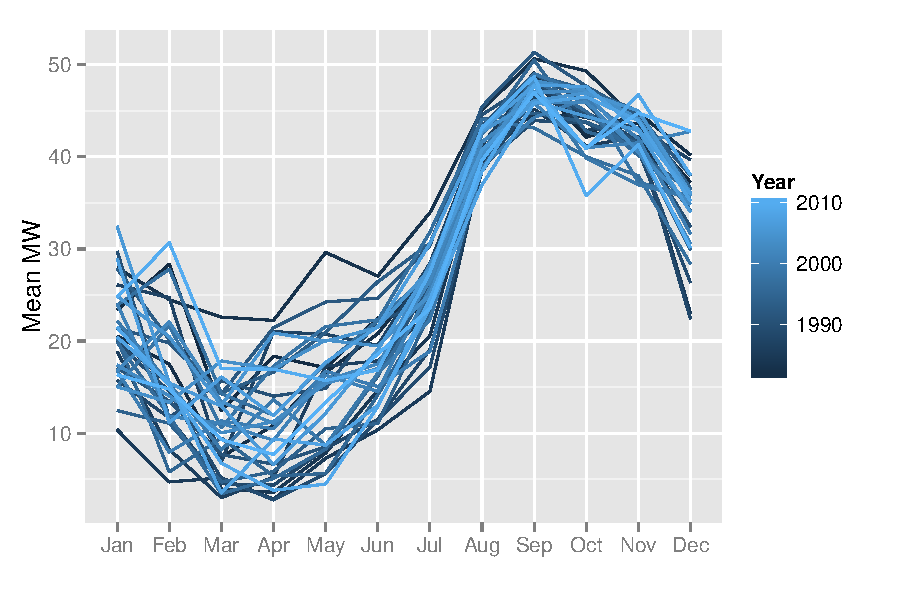
\includegraphics[width=0.8\linewidth]{./Figuras/Icaraizinho/icaraizinho-mensal}
%	\caption{Icaraizinho yearly data. Each serie consists of monthly observations for each year.}
%	\label{fig:icaraizinho-mensal}
%\end{figure}

%
%\begin{figure}
%  \centering
%  \begin{minipage}[t]{1.2\linewidth}
%    \begin{minipage}[t]{0.45\linewidth}
%       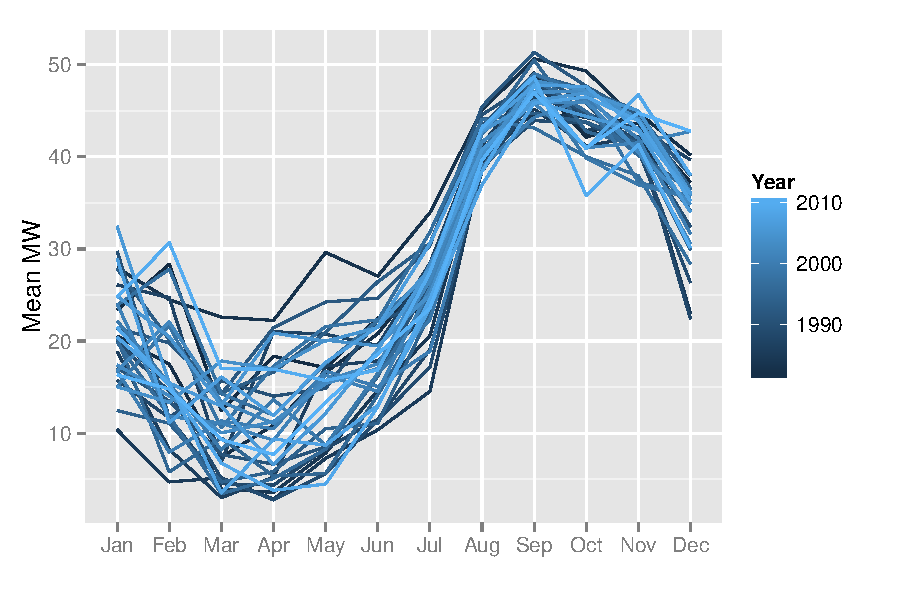
\includegraphics[width=\textwidth]{./Figuras/Icaraizinho/icaraizinho-mensal}
%      	%\caption{Boxplot for each month for the Icaraizinho dataset}
%      	\label{fig:icaraizinho-boxplot}
%    \end{minipage}
%    \begin{minipage}[t]{0.45\linewidth}
%       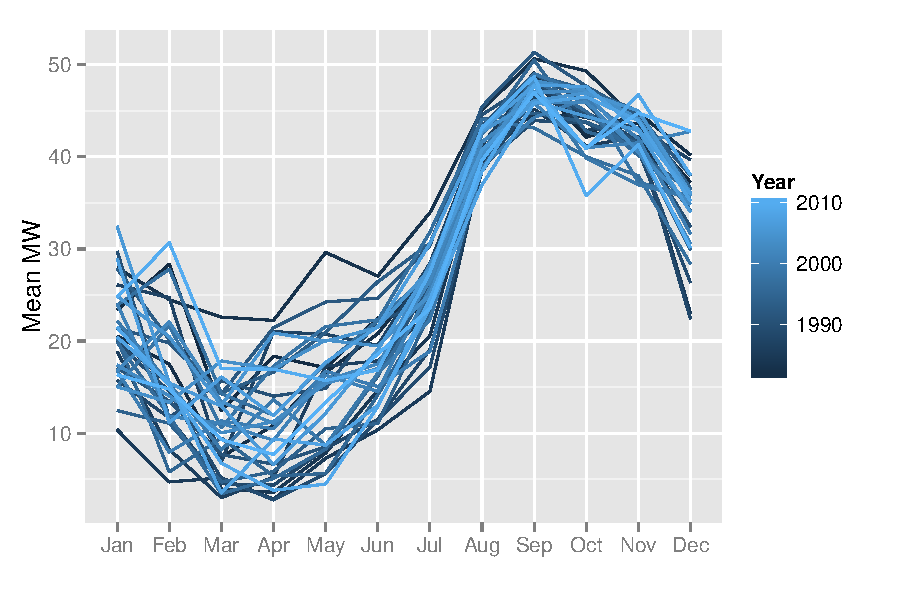
\includegraphics[width=\textwidth]{./Figuras/Icaraizinho/icaraizinho-mensal}
%      	%\caption{Boxplot for each month for the Icaraizinho dataset}
%      	\label{fig:tubarao-boxplot}
%    \end{minipage}
%  \end{minipage}
%  \caption{Relationship between $y_t$ and some chosen lags.}
%  \label{fig:boxplots}
%\end{figure}


In this work, we apply a few different techniques to forecast the quantile function a few steps ahead. The main frameworks we investigate are parametric linear models and a non-parametric regression. We also investigate how to apply quantile estimations to produce an empirical distribution for the $k$-step ahead forecasting by using a nonparametric approach.
%To study our methods performance, we use the mean power monthly data of Icaraizinho, a wind farm located in the Brazilian northeast, and solar.

%The Icaraizinho dataset consists of monthly observations from 1981 to 2011 of mean power measured in Megawatts. The full Icaraizinho serie can be found on the appendices from this article.  As is common in renewable energy generation, there is a strong seasonality component. Figures \ref{fig:icaraizinho-mensal} and \ref{fig:icaraizinho-boxplot} illustrate this seasonality, where we can observe low amounts of power generation for the time span between February and May, and a yearly peek between August and November.

To make good predictions of random variables, one must find good explanatory variables: it can be either autoregressive, exogenous terms or even a deterministic function that repeats itself.
Figure \ref{fig:scatterplot-1lag} shows scatter plots relating $y_t$ with its first lag for both short and long term. We can see that in both of them past values are good explanatory variables to use for forecasting.

\begin{figure}
  \centering
  \begin{minipage}[t]{\linewidth}

    \begin{minipage}[t]{0.45\linewidth}
      %\centering
       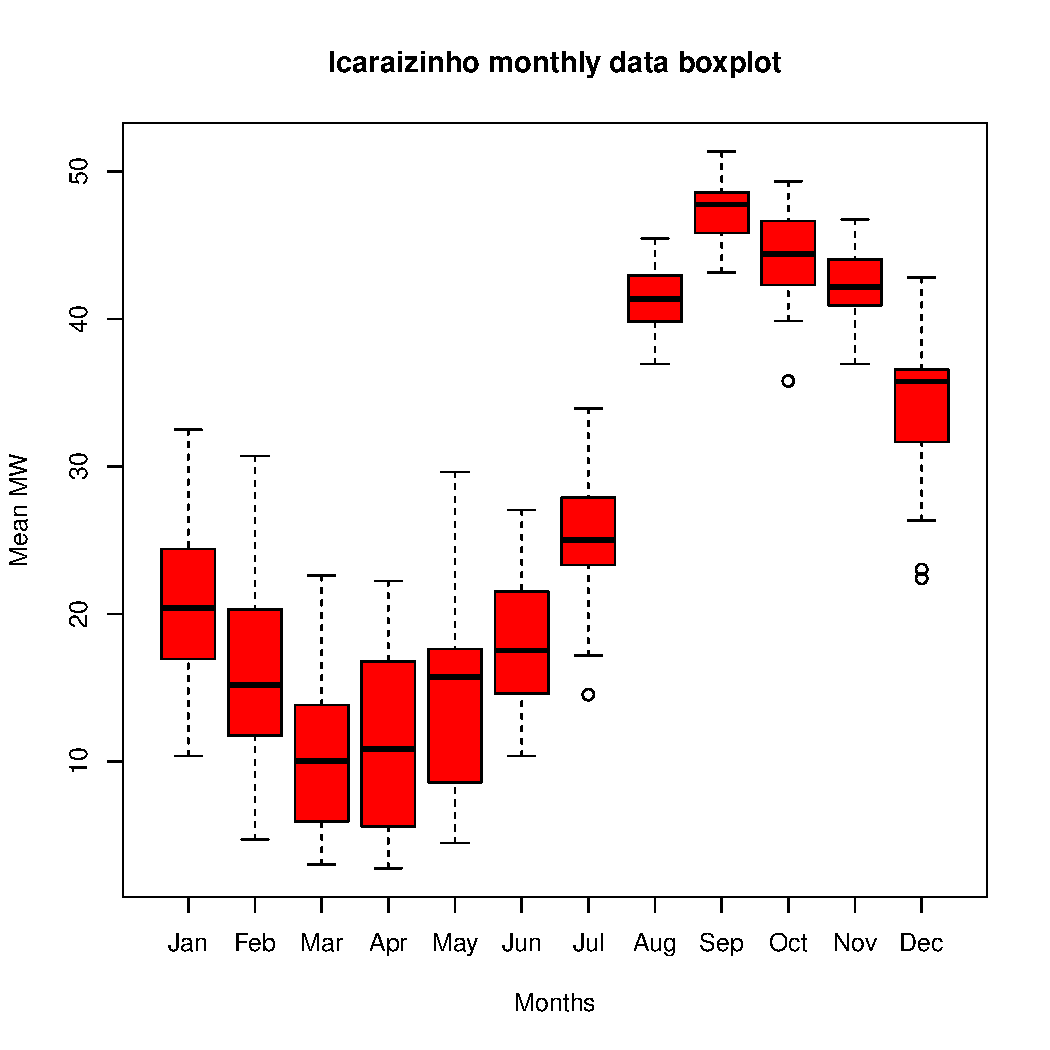
\includegraphics[width=\textwidth]{./Figuras/Icaraizinho/icaraizinho-boxplot}
      	%\caption{Boxplot for each month for the Icaraizinho dataset}
      	\label{fig:icaraizinho-boxplot}
    \end{minipage}
    \begin{minipage}[t]{0.45\linewidth}
      %\centering
       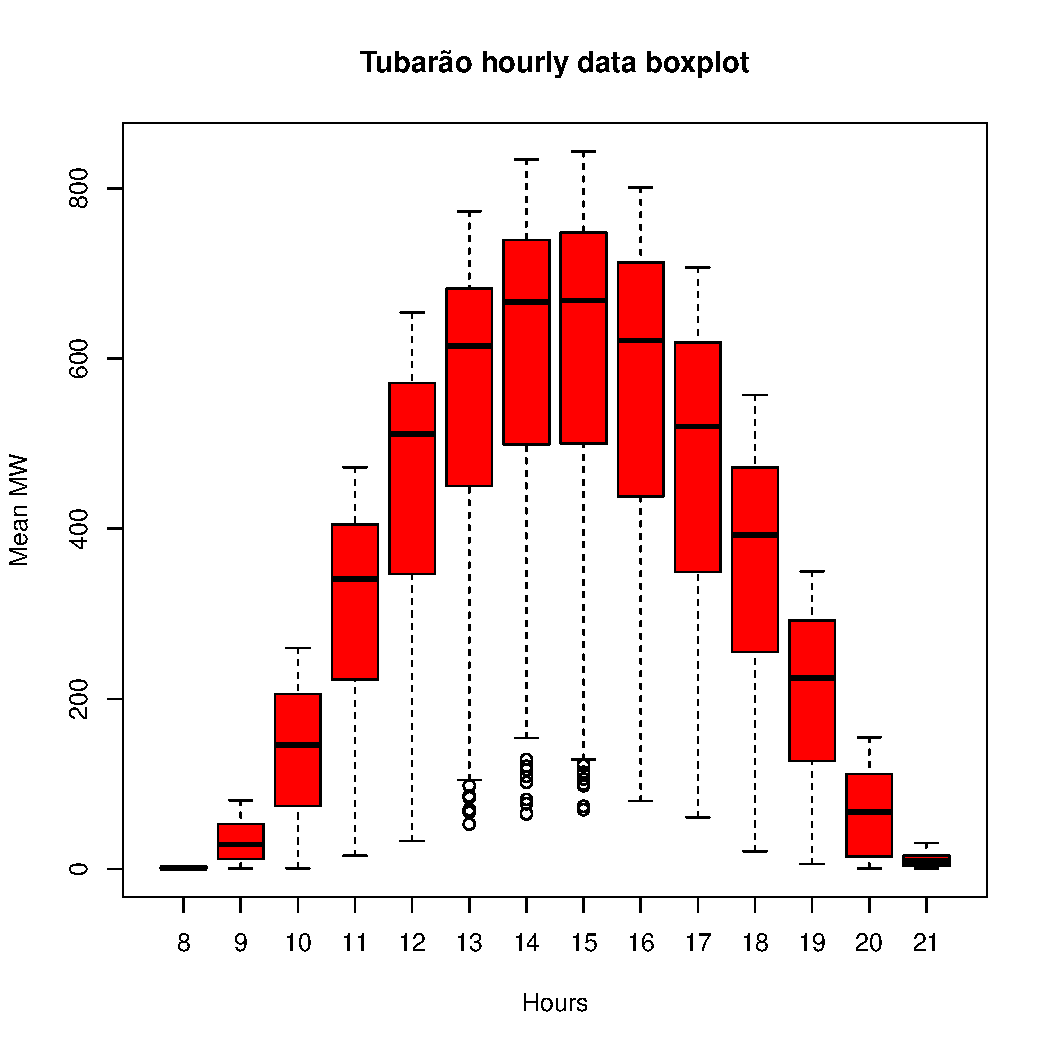
\includegraphics[width=\textwidth]{./Figuras/Solar-exemplos/tubarao-boxplot}
      	%\caption{Boxplot for each month for the Icaraizinho dataset}
      	\label{fig:tubarao-boxplot}
    \end{minipage}
  \end{minipage}
  \caption{Boxplots showing seasonality for monthly and hourly data.}
  \label{fig:boxplots}
\end{figure}



\begin{figure}
  \centering
  \begin{minipage}[t]{\linewidth}
    \centering
    \begin{minipage}[t]{0.45\linewidth}
      \centering     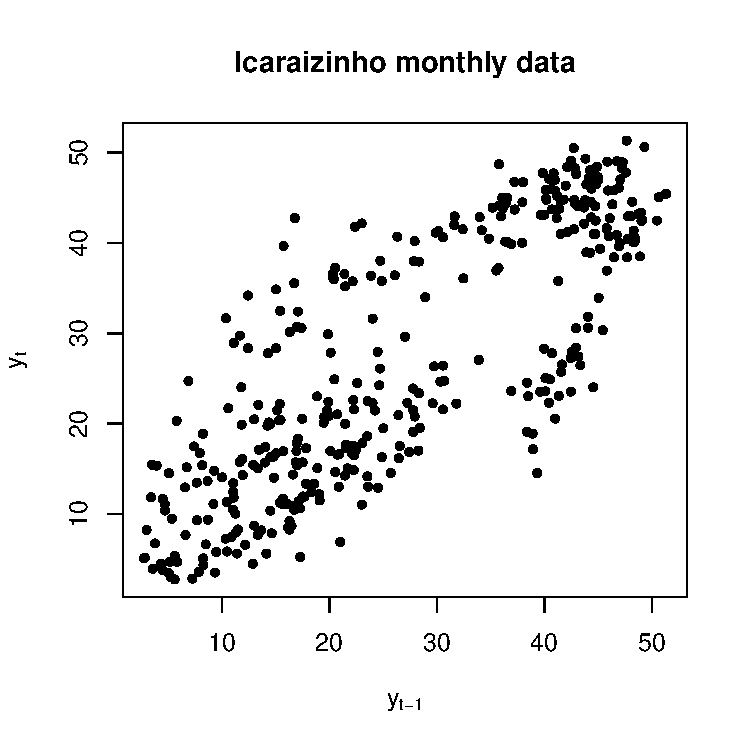
\includegraphics[width=\textwidth]{Figuras/Icaraizinho/scatterplot.pdf}
    \end{minipage}
    \begin{minipage}[t]{0.45\linewidth}
      \centering     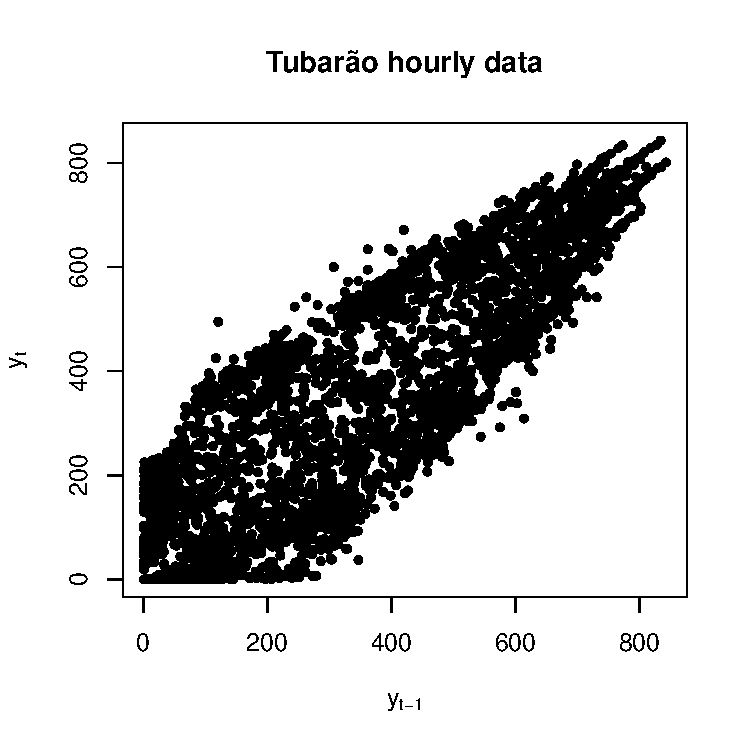
\includegraphics[width=\textwidth]{Figuras/Solar-exemplos/scatterplot}
    \end{minipage}
  \end{minipage}
  \caption{Relationship between $y_t$ and its first lags for two selected series.}
  \label{fig:scatterplot-1lag}
\end{figure}

In contrast to the linear regression model through ordinary least squares (OLS), which provides only an estimation of the dependent variable conditional mean, quantile regression model yields a much more detailed information concerning the complex relationship about the dependent variable and its covariates. Here we denote as parametric linear model the well-known quantile regression model \cite{koenker2005quantile}.

Let $Y$ be a real valued random variable. The quantile function $Q_Y:[0,1] \rightarrow \mathbb{R}$ is defined pointwise by its $\alpha$-quantile, which is given by
\begin{equation}
Q_Y(\alpha) = F_Y^{-1}(\alpha) = \inf\{y: F_Y(y) \geq \alpha\},
\label{eq:quantile-function}
\end{equation}
where $F_Y$ is the distribution function of random variable $Y$ and $\alpha \in [0,1]$. Equation \ref{eq:quantile-function} defines what we call from now on as the quantile function $Q_Y(\cdot)$, in relation to random variable $Y$. In this article, we are interested in a conditional quantile function $Q_{Y|X=x}(\alpha, x)$ (in short, from now on, $Q_{Y|X}(\alpha, x)$), where $X$ can be a vector.

Let $(\Omega, \mathcal{F}, P)$ be a probability space. The conditional quantile function can be found as the result of the following optimization problem:
\begin{eqnarray}
Q_{Y|X}(\alpha,x)\quad & \in\quad\underset{q_\alpha(\cdot)}{\text{arg min}}\, &
(1-\alpha)\int_{\omega \in \Omega}|Y(w)-q_\alpha(X(w))|^{-}P(dw) \label{eq:optim-continuous}
 \\ & & + (\alpha)\int_{\omega \in \Omega}|Y(w)-q_\alpha(X(w))|^{+}P(dw) \nonumber
\end{eqnarray}

\begin{equation}
  q_\alpha  \in \mathcal{Q},
\end{equation}
where $A$ is a set containing a sequence of probabilities  $\alpha_i$ such that $0 < \alpha_1 < \alpha_2 < \dots < \alpha_Q < 1$. This set represents a finite discretization of the interval $[0,1]$. These values must be close enough so that $Q_{Y|X}(\alpha)$ has a precise representation. The argument of optimization problem described on equation \ref{eq:optim-continuous} is the function $q_\alpha$, which belongs to a function space $\mathcal{Q}$. We might have different assumptions for the space $\mathcal{Q}$, depending on the type of function we want to find for $q_\alpha$. A few properties, however, must be achieved by our choice. The conditional quantile function $Q_{Y|X}(\alpha)$ must be monotone on $\alpha$, and its first derivative must be limited.

In this work, we use the sample quantile,  where we calculate the optimization based on a finite number of observations, instead of integrating over all domain of random variable $Y$. For the specific case where the random variable is a time series $y_t$, quantiles are estimated from a $n$ size sample of observations of $y_t$ and a explanatory variable $x_t$ for each $t$, such that our random sample is formed by the sequence $\{y_t,x_t \}_{t=1}^n$. To estimate the $\alpha$-quantile from a sample, we change \ref{eq:optim-continuous} for the following optimization problem:
\begin{equation}
\hat{Q}_{Y|X}(\alpha,x)\quad \in\quad\underset{q_\alpha(\cdot)}{\text{arg min}}\,\sum_{t=1}^{n}\alpha|y_{t}-q_\alpha(x_t)|^{+}+\sum_{t=1}^{n}(1-\alpha)|y_{t}-q_\alpha(x_t)|^{-},
\label{eq:linear-model}
\end{equation}
\begin{equation}
  q_\alpha  \in \mathcal{Q},
\end{equation}
where $q_\alpha(x_t)$ is the estimated quantile value at a given time $t$ and $|x|^+=\max\{0,x\}$ and $|x|^-=-\min\{0,x\}$. The solution from the above problem is an estimator $\hat{Q}_{Y|X}$ for the quantile function $Q_{Y|X}$.

To model this problem as a Linear Programming problem, thus being able to use a modern solver to fit our model,  we create variables $\varepsilon^+_t$ e $\varepsilon^-_t$ to represent $|y-q(x_t)|^+$ and $|y-q(x_t)|^-$, respectively. The optimal argument $q_\alpha^*(\cdot)$ on the Linear Programming problem \ref{eq:qar-general} is the estimated $\alpha$-quantile for the given random sample.
\begin{equation}
\begin{aligned}\min_{q_\alpha (\cdot),\varepsilon_{t}^{+}, \varepsilon_{t}^{-}} & \sum_{t=1}^{n}\left(\alpha \varepsilon_{t}^{+}+(1-\alpha)\varepsilon_{t}^{-}\right) & \\
\mbox{s.t. } & \varepsilon_{t}^{+}-\varepsilon_{t}^{-}=y_{t}-q_\alpha(x_{t}), & \qquad\forall t \in \{1,\dots,n\},\\
& \varepsilon_t^+,\varepsilon_t^- \geq 0, & \qquad \forall t \in \{1,\dots,n\}.
\end{aligned}
\label{eq:qar-general}
\end{equation}

One of our goals with quantile regression is to estimate a quantile function $\hat{Q}_{Y|X}$ of a given real valued random variable $X$ from a sequence of quantiles $q_{\alpha_1}(x_t) \leq q_{\alpha_2}(x_t) \leq \dots \leq q_{\alpha_{|A|}}(x_t)$, with $0 < \alpha_1 < \alpha_2 < \dots < \alpha_{|A|} < 1$, for any given $t$.
The process of fitting $\hat{Q}_Y$ is by mapping every $\alpha_i$ with its estimated quantile $\hat{q}_{\alpha_i}(x_t)$.
When this sequence of chosen $\alpha_i$ is thin enough, we have a good approximation of $Q_{Y|X}$.
Thus, the distribution found for $Y$ is nonparametric, as no previous assumptions are made about its shape, and its form is fully recovered by the data we have.

A typical problem, however, arises when working with quantile regression. When quantiles are estimated independently, it is possible to find $q_{\alpha}(x_t) > q_{\alpha'}(x_t)$, for a given $t$, when $\alpha_1 < \alpha_2$. An example can be seen on Figure \ref{fig:crossing-quantiles}, where quantiles $\alpha = 0.95$ and $\alpha = 0.9$ cross. This problem, called \textit{crossing quantiles}, can be prevented by estimating all quantiles with a single minimization problem.
\begin{figure}
	\centering
	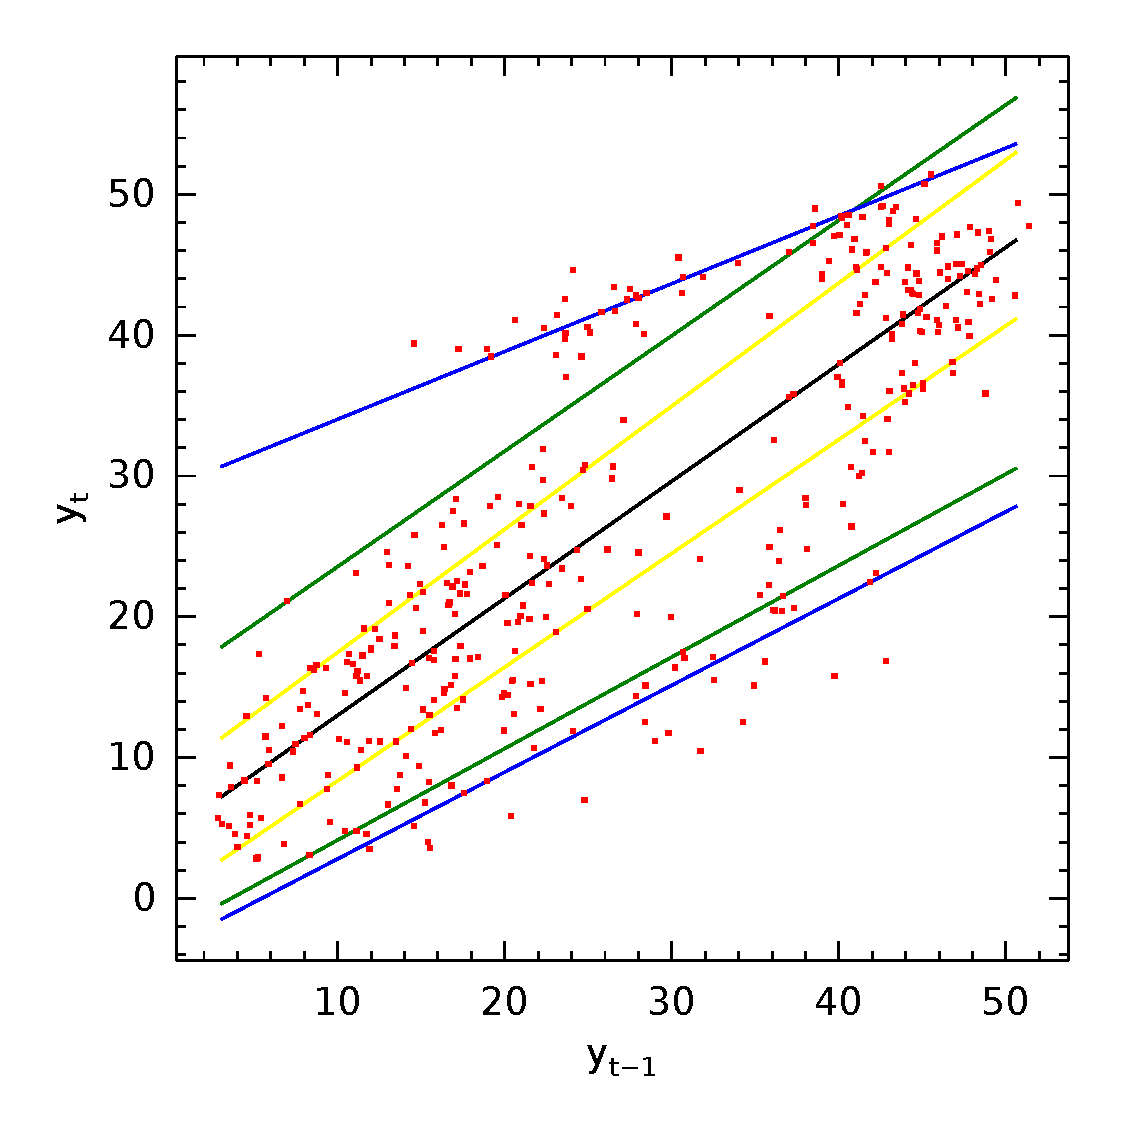
\includegraphics[width=0.6\linewidth]{./Figuras/npqar/icaraizinho-crossing-200}
	\caption{Linear quantile estimator with crossing quantiles for $\alpha = 0.95$ and $\alpha = 0.9$}
	\label{fig:crossing-quantiles}
\end{figure}

 Let $T_n = \{1, 2, \dots, n\}$. In order to estimate all quantiles simultaneously, the new objective function will be the sum of all individual objective functions, as well as include all constraints from all individual problems. The only difference is the inclusion of an equation to guarantee that quantiles won't cross. When modifying problem \ref{eq:qar-general} to account for all quantiles, we have the following new problem:
\begin{eqnarray}
\label{eq:non-crossing-quantiles1}
\min_{q_\alpha(\cdot),\varepsilon_{t,\alpha}^{+}, \varepsilon_{t,\alpha}^{-}} &  \sum_{\alpha \in A} \sum_{t \in T_n}\left(\alpha \varepsilon_{t,\alpha}^{+}+(1-\alpha)\varepsilon_{t,\alpha}^{-}\right) &  \\
\mbox{s.t. } & \varepsilon_{t,\alpha}^{+}-\varepsilon_{t,\alpha}^{-}=y_{t}-q_\alpha(x_{t}), & \qquad\forall t \in T_\tau,\forall \alpha \in A,\\
& \varepsilon_{t,\alpha}^+,\varepsilon_{t,\alpha}^- \geq 0, & \qquad\forall t \in T_\tau,\forall \alpha \in A,\\\label{eq:non-crossing-constraint}
& q_{\alpha}(x_t) \leq q_{\alpha'}(x_t), & \qquad \forall t \in T_\tau, \forall (\alpha, \alpha') \in AxA,  \alpha' \geq \alpha,
\end{eqnarray}
where constraint \ref{eq:non-crossing-constraint} assures that no lower quantile will have a bigger value than a higher quantile.




The next section discusses with bigger details how to fit a distribution function $Q_{Y|X}(\alpha,x)$ from a sequence of estimated quantiles, as well as showing two different strategies to estimate them: linear models and nonparametric models. In the former, $q_\alpha$ is a linear function of an explanatory variable $x_t$.
In the latter, we let $q_\alpha(x_t)$ assume any functional form. To prevent overfitting, however, we penalize the function's roughness by incorporating a penalty on the second derivative.

In section \ref{sec:simulation} we investigate how to simulate $S$ scenarios of $y_t$, considering a linear model and errors $\varepsilon_t$ for which the distribution is unknown. To address this issue, we use quantile linear regression to calculate a thin grid of quantiles and fit a distribution function $\hat{F}_{y_t}$. This function will be used to simulate the innovations on the model.

\section{Estimating distribution function from quantile regressions}
\label{sec:estimating-distribution}

In many applications where a time series model is employed, we often consider the innovations' distribution as known. Take, for example, the AR(p) model:
$$Y=c+\sum_{i=1}^{p}\phi_{i}X_i+\varepsilon_{t},$$
where $X_i$ is a past value of random variable $Y$.
In this model, errors $\varepsilon_t$ are assumed to have normal distribution with zero mean. 

When we are dealing with natural resources data, however, we can't always assume normality. In these cases, one can either find a distribution that has a better fit to the data or have a nonparametric method to estimate the distribution directly from the available data.

In a time series framework, where a time series $y_t$ is given by a linear model of its regressors $x_t$
$$Y_t = \beta^T X_t + \varepsilon_t,$$
we propose to estimate the $k$-step ahead distribution of $Y_t$ with a nonparametric approach.
Let an empirical $\alpha$-quantile $\hat{q}_\alpha \in \mathcal{Q}$ be a functional belonging to a functional space. In any given $t$, we can estimate the sequence of quantiles $\{ q_{\alpha}(x_t) \}_{\alpha \in A}$ by solving the problem defined on equations (\ref{eq:non-crossing-quantiles1})-(\ref{eq:non-crossing-constraint}). 
 After evaluating this sequence, by making equal 
\begin{equation}
\hat{Q}_{y_t|X=x_t}(\alpha) = \hat{q}_\alpha(x_t), \qquad \forall \alpha \in A,
\end{equation}
we have a set of size $|A|$ of values to define the discrete function over the first argument $\hat{Q}_{y_t|x_t}(\alpha,X=x_t): A \times \mathbb{R}^d \rightarrow \mathbb{R}$. The goal of having function $\hat{Q}$ is to use it as base to construct the estimated quantile function $\hat{Q}'_{y_t|X=x_t}(\alpha,x_t): [0,1] \times \mathbb{R}^d \rightarrow \mathbb{R}$. 

A problem arises for the distribution extremities, because when $\alpha = 0$ or $\alpha = 1$, the optimization problem becomes unbounded. In order to find values for $\hat{Q}(\alpha,x_t)$ when $\alpha \in \{0,1\}$, we chose to linearly extrapolate its values. %completar com explicação de extrapolação
Note that as $A \subset [0,1]$, the domain of $\hat{Q}$ is also a subset of the domain of $\hat{Q}'$. 
The estimative of $\hat{Q}'$ is done by interpolating points of $\hat{Q}$ over the interval $[0,1]$.
Thus, the distribution found for $\hat{y}_{\tau}$ is nonparametric, as no previous assumptions are made about its shape, and its form is fully recovered by the data we have.


We investigate two different approaches for $Q_{y_t}$ by the functional structure of each individual $q_\alpha(x_t)$.
In section \ref{sec:linear-models}, we explore the case where the individual quantiles $q_\alpha(x_t)$ are a linear function of its arguments:
\begin{equation}
\hat{q}_\alpha(x_t) = \beta_{0,\alpha} +   \beta_\alpha^T x_t,
\label{eq:fun-quantile}
\end{equation}
where $\beta^\alpha$ is a vector of coefficients for the explanatory variables.

In section \ref{sec:npqar} we introduce a Nonparametric Quantile Autoregressive model with a $\ell_{1}$-penalty term, in order to properly simulate densities for several $\alpha$-quantiles. In this nonparametric approach we don't assume any form for $q_\alpha(x_t)$, but rather let the function adjust to the data. To prevent overfitting, the $\ell_1$ penalty for the second derivative (approximated by the second difference of the ordered observations) is included in the objective function. The result of this optimization problem is that each $q_\alpha(x_t)$ will be a function with finite second derivative.

In order to find good estimates for $Q_{y_{t}}(\alpha)$ when $\alpha$ approaches 0 or 1, as well as performing interpolation on the values that were not directly estimated, we can either use a kernel smoothing function, splines, linear approximation, or any other method. 

\section{Linear Models for the Quantile Autoregression}
\label{sec:linear-models}

Given a time series $\{y_t\}$, we investigate how to select which lags will be included in the Quantile Autoregression. We won't be choosing the full model because this normally leads to a bigger variance in our estimators, which is often linked with bad performance in forecasting applications. So our strategy will be to use some sort of regularization method in order to improve performance.
We investigate two ways of accomplishing this goal.
The first of them consists of selecting the best subset of variables through Mixed Integer Programming, given that $K$ variables are included in the model. Using MIP to select the best subset of variables is investigated in \cite{bertsimas2015best}. The second way is including a $\ell_1$ penalty on the linear quantile regression, as in \cite{kim2009ell_1}, and let the model select which and how many variables will have nonzero coefficients. 
Both of them will be built over the standard Quantile Linear Regression model. In the end of the section, we discuss a information criteria to be used for quantile regression and verify how close are the solutions in the eyes of this criteria.

When we choose $q(x_t)$ to be a linear function, as on equation \ref{eq:linear-model} (that we reproduce below for convenience):
\begin{equation}
\min_{f}\sum_{t=1}^{n}\alpha|y_{t}-q(x_t)|^{+}+(1-\alpha)|y_{t}-q(x_t)|^{-},
\end{equation}
we can substitute it on problem \ref{eq:qar-general}, getting the following LP problem:
\begin{equation}
\begin{aligned}\min_{\beta_0,\beta,\varepsilon_{t}^{+},\varepsilon_{t}^{-}} & \sum_{t=1}^{n}\left(\alpha\varepsilon_{t}^{+}+(1-\alpha)\varepsilon_{t}^{-}\right)\\
\mbox{s.t. } & \varepsilon_{t}^{+}-\varepsilon_{t}^{-}=y_{t} - \beta_0 - \beta^T x_{t},\qquad\forall t\in\{1,\dots,n\},\\
& \varepsilon_t^+,\varepsilon_t^- \geq 0, \qquad \forall t \in \{1,\dots,n\}.
\end{aligned}
\label{eq:qar-lp}
\end{equation}

In this work, we didn't explore the addition of terms other than the terms $y_t$ past lags. For example, we could include functions of $y_{t-p}$, such as $log(y_{t-p})$ or $exp(y_{t-p})$. We leave such inclusion for further works. 

\subsection{Best subset selection with Mixed Integer Programming}
\label{sec:best-subset-mip}

In this part, we investigate the usage of Mixed Integer Programming to select which variables are included in the model, up to a limit of inclusions imposed \textit{a priori}. The optimization problem is described below:
\begin{eqnarray}
\min_{\beta_{0},\beta, z,\varepsilon_{t}^{+},\varepsilon_{t}^{-}} &  \sum_{t=1}^{n}\left(\alpha\varepsilon_{t}^{+}+(1-\alpha)\varepsilon_{t}^{-}\right) \\
\mbox{s.t } & \varepsilon_{t}^{+}-\varepsilon_{t}^{-}=y_{t}-\beta_{0}-\sum_{p=1}^{P}\beta_{p}x_{t,p},& \qquad\forall t\in\{1,\dots,n\}, \label{linear1}\\
 & \varepsilon_{t}^{+},\varepsilon_{t}^{-}\geq0,&\qquad\forall t \in \{1,\dots,n\}, \label{linear2}\\
 & - M_U z_p \leq \beta_p \leq M_U z_p,&\qquad\forall p\in\{1,\dots,P\}, \label{linear3}\\
 & \sum_{p=1}^P z_p \leq K, \label{linear4}\\
 & z_p \in \{0,1\},&\qquad\forall p\in\{1,\dots,P\}. \label{eq:linear5}
\end{eqnarray}
The objective function and constraints (\ref{linear2}) and (\ref{linear3}) are those from the standard linear quantile regression. The other constraints implement the process of regularization, forcing a maximum of $K$ variables to be included. By (\ref{linear3}), variable $z_p$ is a binary that assumes 1 when the coefficient $\beta_p$ is included. $M_U$ is chosen in order to guarantee that $M_U \geq \|\hat{\beta}\|_{\infty}$. The solution given by $\beta_0$ and $\beta$ will be the best linear quantile regression with $K$ nonzero coefficients. 

We ran this optimization for each value of $K \in \{1, \dots, 12\}$ and quantiles $\alpha \in \{0.05, 0.1, 0.5, 0.9, 0.95\}$. We could see that for all quantiles the 12\textsuperscript{th} lag was the one included when $K=1$. When $K=2$, the 1\textsuperscript{st} lag was always included, sometimes with $\beta_{12}$, some others with $\beta_4$ and once with $\beta_{11}$. These 4 lags that were present until now are the only ones selected when $K=3$. For $K=4$, those same four lags were selected for three quantiles (0.05, 0.1 and 0.5), but for the others (0.9 and 0.95) we have $\beta_6$, $\beta_7$ and $\beta_9$ also as selected. From now on, the inclusion of more lags represent a lower increase in the fit of the quantile regression. The estimated coefficient values for all $K$'s are available in the appendices section. Figure \ref{fig:icaraizinho-crossing-200} shows a linear estimator for the quantiles $(0.05, 0.1, 0.25, 0.5, 0.75, 0.9, 0.95)$.

\begin{figure}
\centering
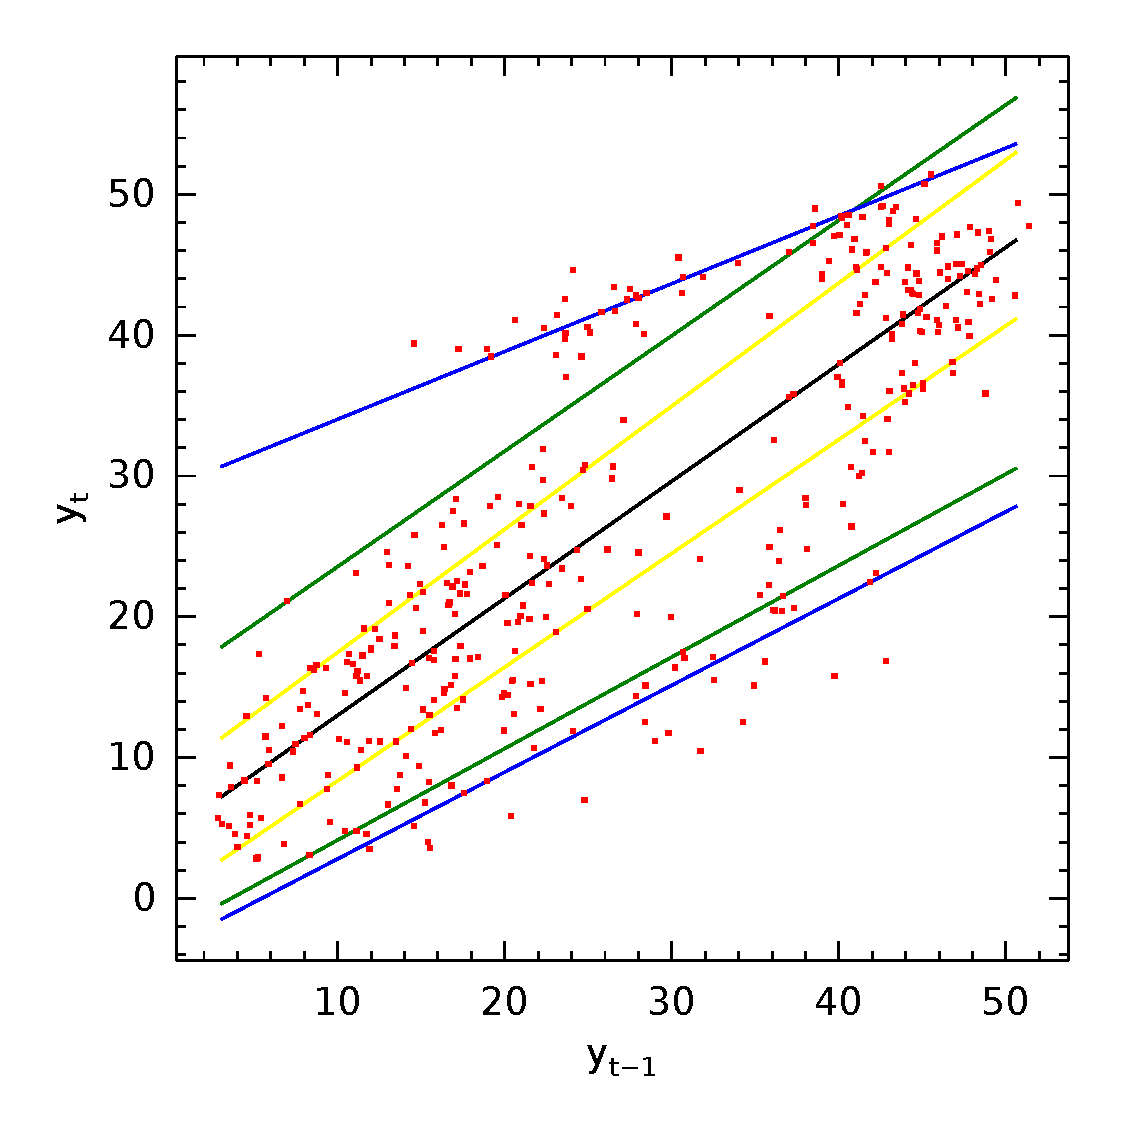
\includegraphics[width=0.7\linewidth]{Figuras/npqar/icaraizinho-crossing-200}
\caption{Linear Quantile Regression when only $y_{t-1}$ is used as explanatory variable}
\label{fig:icaraizinho-crossing-200}
\end{figure}


\subsection{Best subset selection with a $\ell_1$ penalty}
\label{sec:best-subset-ell1}

Another way of doing regularization is including the $\ell_1$-norm of the coefficients on the objective function. The advantage of this method is that coefficients are shrunk towards zero, and only some of them will have nonzero coefficients. By lowering the penalty we impose on the $\ell_1$-norm, more variables are being added to the model. 
This is the same strategy of the LASSO, and its usage for the quantile regression is discussed in \cite{li2012l1}.
The proposed optimization problem to be solved is:

\begin{equation}
\min_{\beta_{0},\beta}\sum_{t=1}^{n}\alpha|y_{t}-q(x_t)|^{+}+(1-\alpha)|y_{t}-q(x_t)|^{-}+\lambda\|\beta\|_{1}
\label{eq:l1-qar-optim}
\end{equation}
\[
q(x_t)=\beta_{0}-\sum_{p=1}^{P}\beta_{p}x_{t,p},
\]
where the regressors $x_{t,p}$ used are its lags. In order to represent the above problem to be solved with linear programming solver, we restructure the problem as below:
\begin{eqnarray}
\beta_\lambda^{*LASSO} = \argmin_{\beta_{0},\beta,\varepsilon_{t}^{+},\varepsilon_{t}^{-}} & \sum_{i=1}^{n}\left(\alpha\varepsilon_{t}^{+}+(1-\alpha)\varepsilon_{t}^{-}\right)+\lambda\sum_{p=1}^{P}\mbox{\ensuremath{\xi}}_{p} \label{eq:obj-lasso} \\
\mbox{s.t. } & \varepsilon_{t}^{+}-\varepsilon_{t}^{-}=y_{t}-\beta_{0}-\sum_{p=1}^{P}\beta_{p}x_{t,p},\qquad\forall t\in\{1,\dots,n\},\\
 & \varepsilon_{t}^{+},\varepsilon_{t}^{-}\geq0,\qquad\forall t \in \{1,\dots,n\},\\
 & \xi_{p}\geq\beta_{p},\qquad\forall p\in\{1,\dots,P\}, \label{l1-qar-3}\\
 & \xi_{p}\geq-\beta_{p},\qquad\forall p\in\{1,\dots,P\}, \label{l1-qar-4}
\end{eqnarray}
Once again, this model is built upon the standard linear programming model for the quantile regression (equation \ref{eq:qar-lp}). 
On the above formulation, the $\ell_1$ norm of equation (\ref{eq:l1-qar-optim}) is substituted by the sum of $\xi_p$, which represents the absolute value of $\beta_p$. The link between variables $\xi_p$ and $\beta_p$ is made by constraints (\ref{l1-qar-3}) and (\ref{l1-qar-4}). Note that the linear coefficient $\beta_0$ is not included in the penalization, as the sum of penalties on the objective function \ref{eq:obj-lasso}.

For such estimation to produce good results, however, each variable must have the same relative weight in comparison with one another. So, before solving the optimization problem, we normalize all variables to have mean $\mu = 0$ and variance $\sigma^2 = 1$. For the vector of observations for each covariate (that in our problem represents is a vector of observations of lags $y_{t-p}$), we apply the transformation $\tilde{y}_{t-p,i} = (y_{t-p,i} - \bar{y}_{t-p}) / \sigma_{t-p}$, where $\bar{y}_{t-p}$ is the $p$-lag mean and $\sigma_{t-p}$ the $p$-lag standard deviation. We use the $\tilde{y}_{t-p,i}$ series to estimate the coefficients. Once done that, we multiply each coefficient for its standard deviation to get the correct coefficient: $\beta_i = \tilde{\beta}_i \dot \sigma_{t-p}$.

For low values of $\lambda$, the penalty is small and thus we have a model where all coefficients have a nonzero value. On the other hand, while $\lambda$ is increased the coefficients shrink towards zero; in the limit we have a constant model. For instance, we don't penalize the linear coefficient $\beta_0$. For the same quantiles values $\alpha$ we experimented on section \ref{sec:best-subset-mip} ($\alpha \in \{0.05, 0.1, 0.5, 0.9, 0.95\}$). 


\begin{figure}
  \centering
  \begin{minipage}[t]{0.4\linewidth}
    \centering
    \begin{minipage}[t]{\linewidth}
      \centering     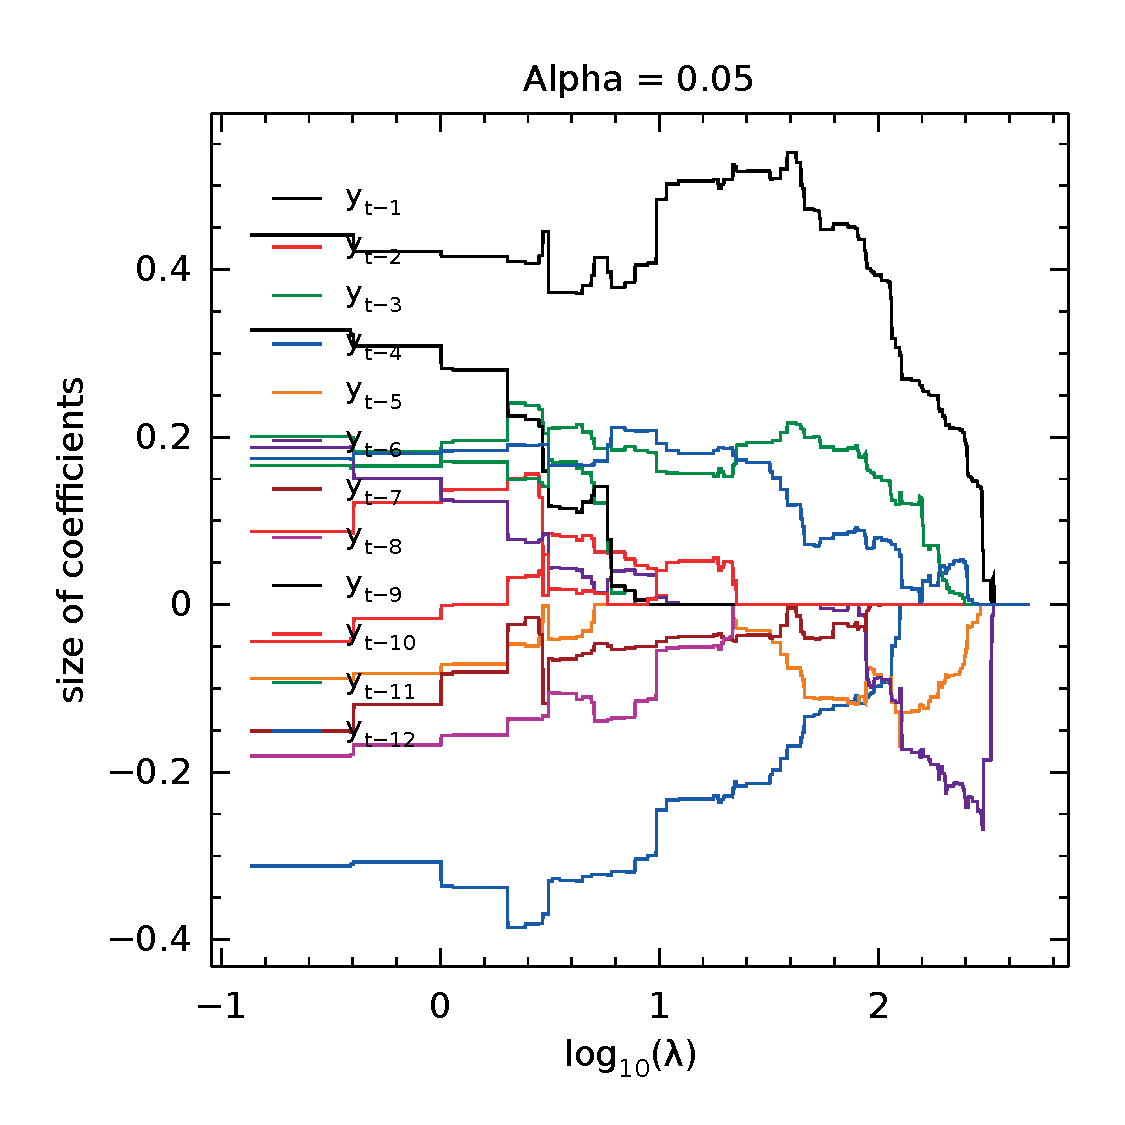
\includegraphics[width=\textwidth]{Figuras/selecao-lasso/par-sellasso-005.pdf}
    \end{minipage}
    \begin{minipage}[b]{\linewidth}
      \centering     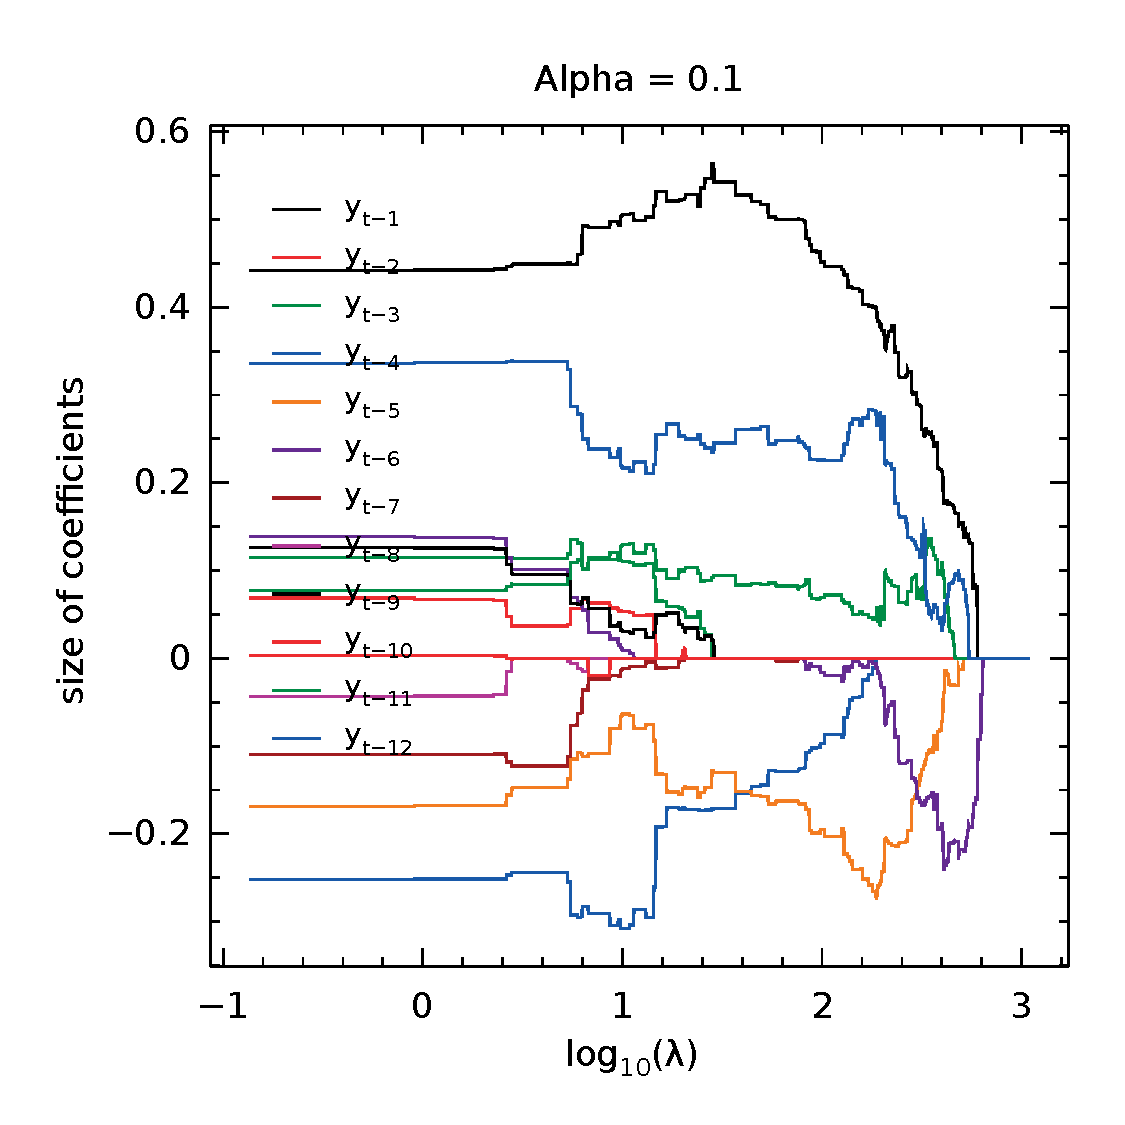
\includegraphics[width=\textwidth]{Figuras/selecao-lasso/par-sellasso-01.pdf}
    \end{minipage}
     \begin{minipage}[b]{\linewidth}
      \centering     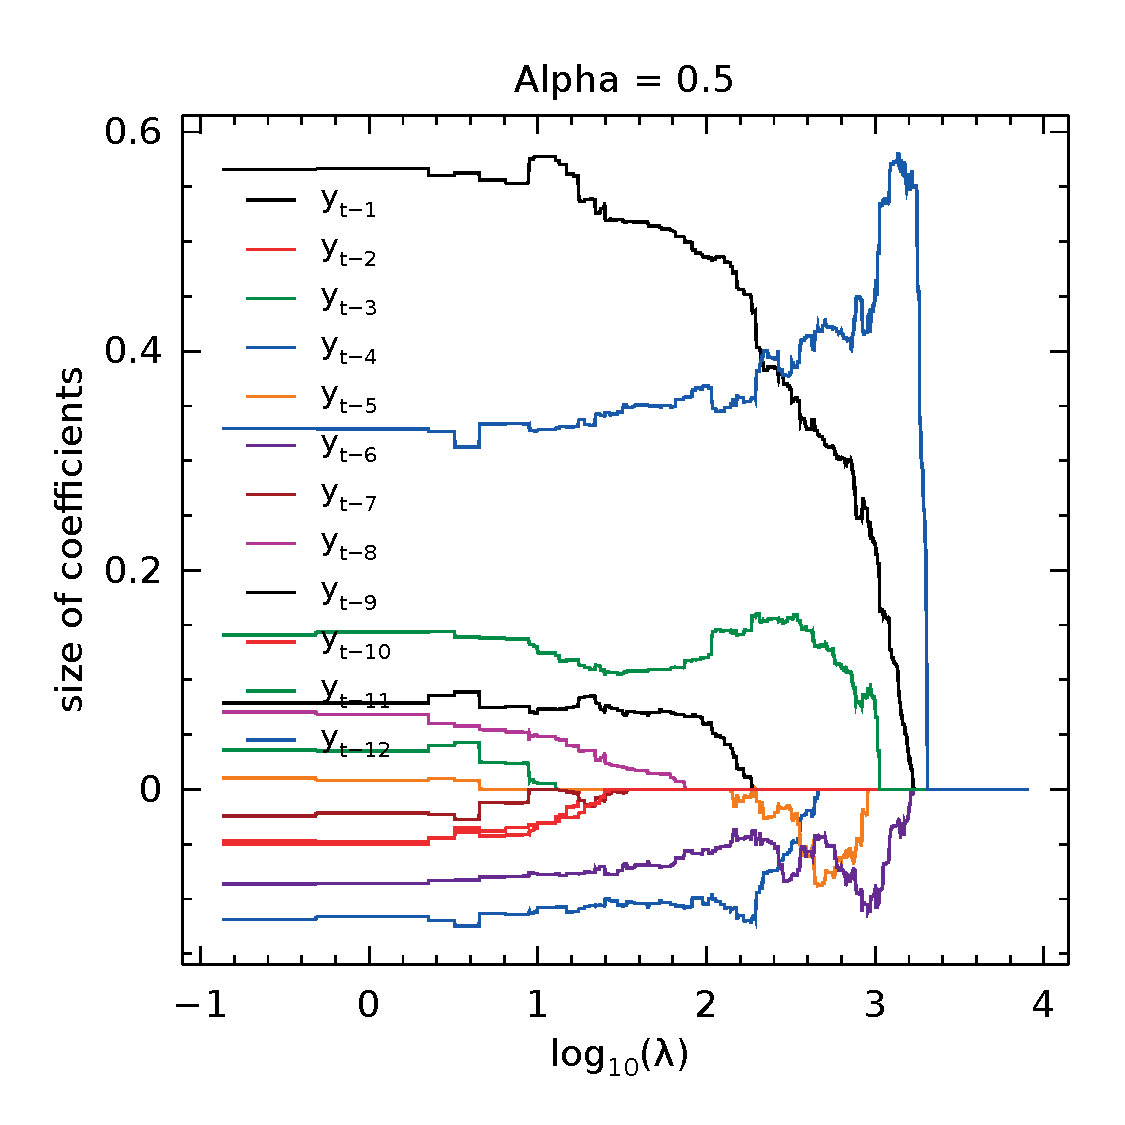
\includegraphics[width=\textwidth]{Figuras/selecao-lasso/par-sellasso-05.pdf}
     \end{minipage}
  \end{minipage}
  \begin{minipage}[t]{0.4\linewidth}
    \centering
    \begin{minipage}[b]{\linewidth}
      \centering     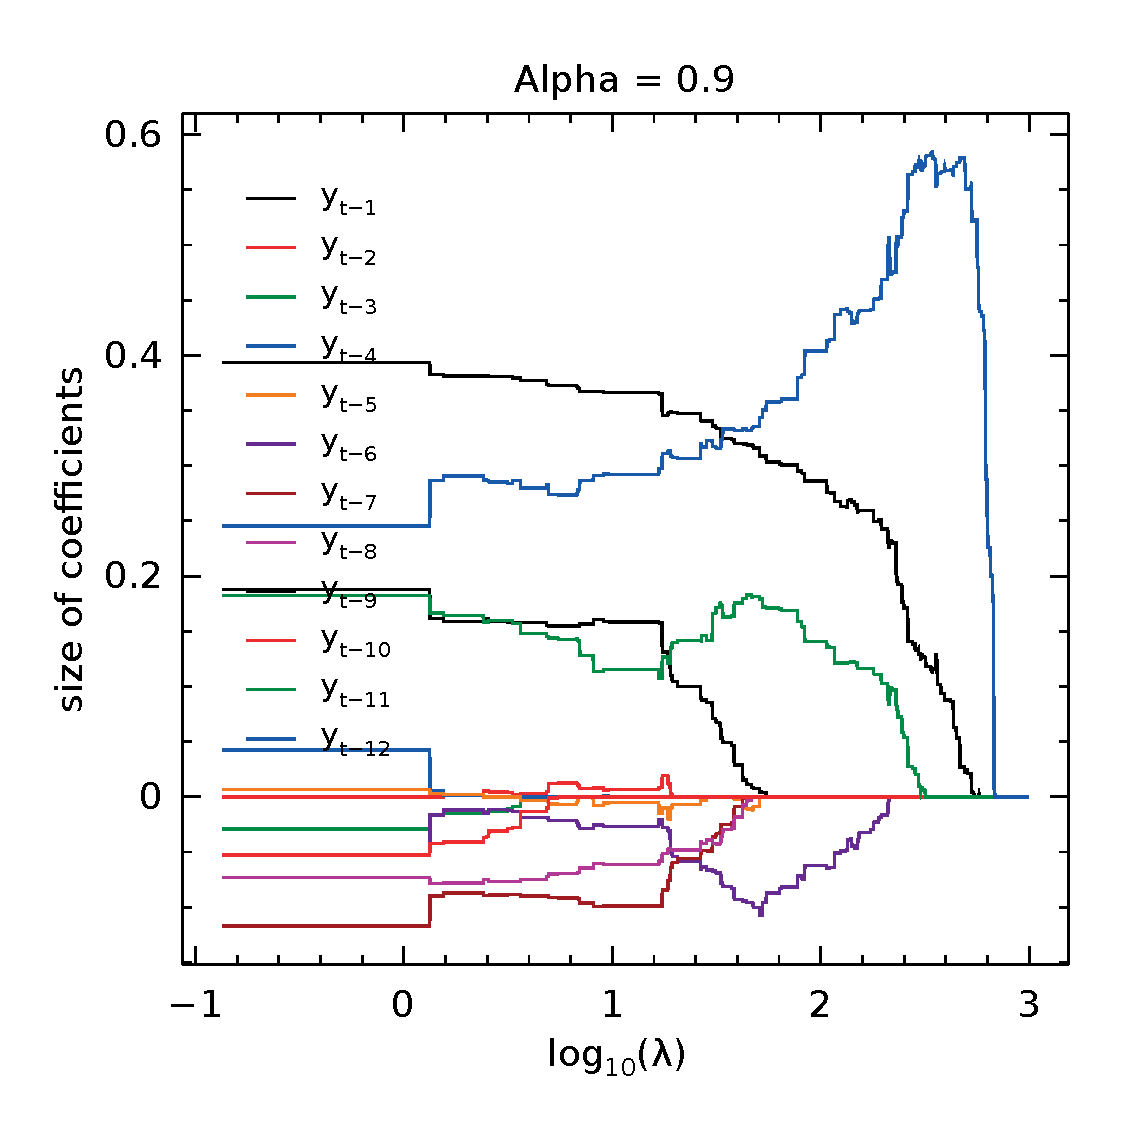
\includegraphics[width=\textwidth]{Figuras/selecao-lasso/par-sellasso-09.pdf}
    \end{minipage}
     \begin{minipage}[b]{\linewidth}
      \centering     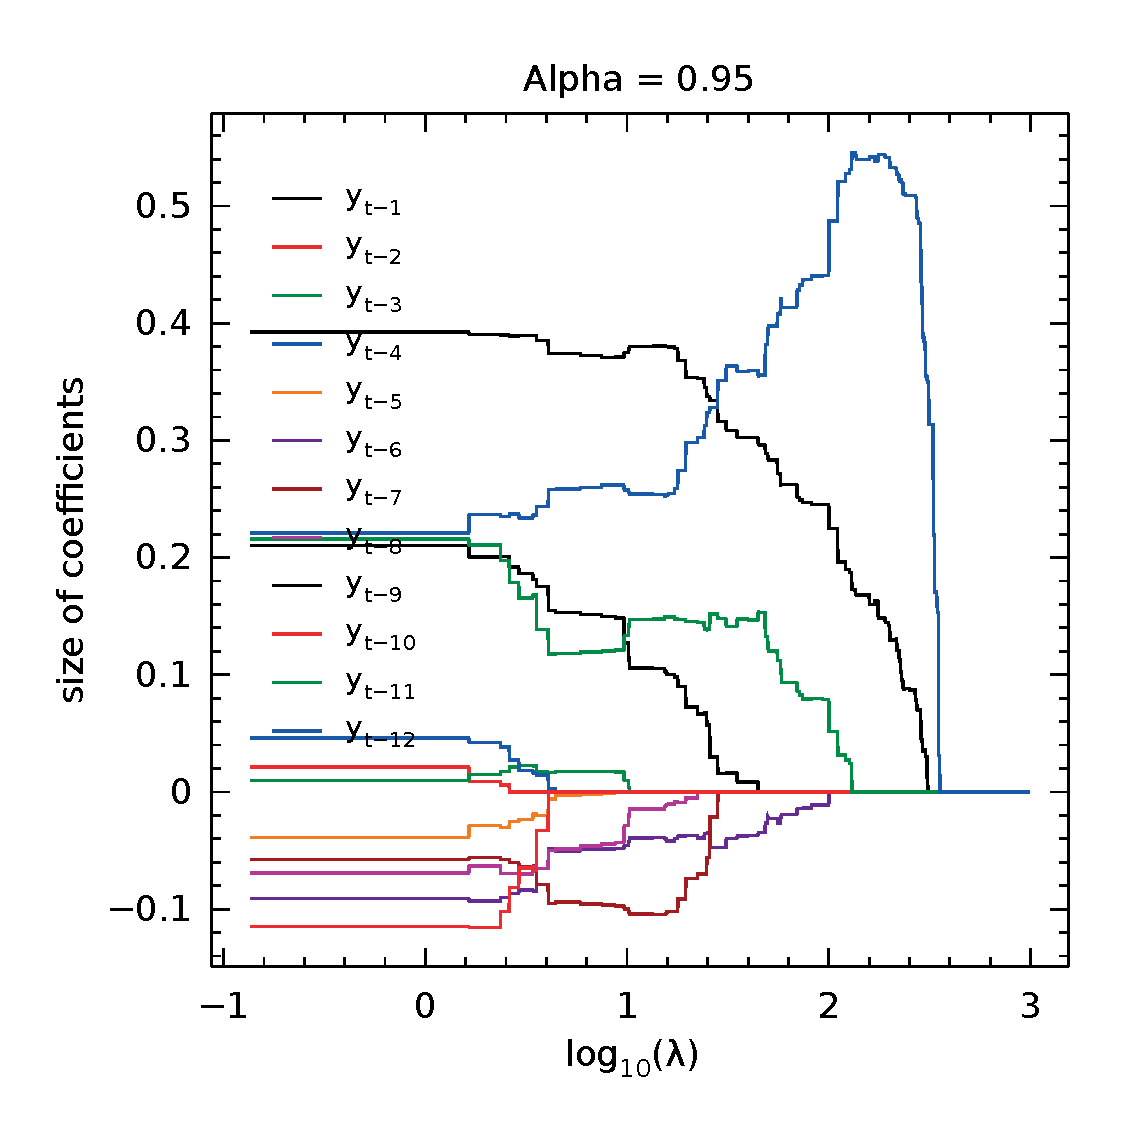
\includegraphics[width=\textwidth]{Figuras/selecao-lasso/par-sellasso-095.pdf}
      \label{fig:npqar-cross}
     \end{minipage}
  \end{minipage}
  \caption{Coefficients path for a few different values of $\alpha$-quantiles. $\lambda$ is presented in a $\log_{10}$ scale, to make visualization easier.}
  \label{fig:npqar-results}
\end{figure}

It is important to mention that even though we have coefficients that are estimated by this method, we don't use them directly. Instead, the nonzero coefficients will be the only covariates used as explanatory variables of a regular quantile autoregression, solved by the linear programming problem \ref{eq:qar-lp}. In summary, the optimization in equation \ref{eq:l1-qar-optim} acts as a variable selection for the subsequent estimation, which is normally called the post-lasso estimation \cite{belloni2009least}.

We are interested, finally, in finding the post-lasso coefficients $\beta_\lambda^*$, which is the solution of the optimization problem given below:
\begin{equation}
\begin{aligned} \beta_\lambda^{*} = \argmin_{\beta_0,\beta,\varepsilon_{t}^{+},\varepsilon_{t}^{-}} & \sum_{t=1}^{n}\left(\alpha\varepsilon_{t}^{+}+(1-\alpha)\varepsilon_{t}^{-}\right)\\
\mbox{s.t. } & \varepsilon_{t}^{+}-\varepsilon_{t}^{-}=y_{t} - \beta_0 - \sum_{p\in L_\lambda} \beta_p x_{t,p},\qquad\forall t\in\{1,\dots,n\},\\
& \varepsilon_t^+,\varepsilon_t^- \geq 0, \qquad \forall t \in \{1,\dots,n\}.
\end{aligned}
\label{eq:post-lasso}
\end{equation}
Note that only a subset of the $P$ covariates will have nonzero values, which are given by the set 
\begin{equation*}
L_\lambda = \{ p \; | \; p \in \{ 1,\dots,P \}, \; |\beta^{*LASSO}_{\lambda,p}| \neq 0  \}.
\end{equation*}
Hence, we have that
$$\beta^{*LASSO}_{\lambda,p} = 0 \iff \beta^{*}_{\lambda,p} = 0.$$


\subsection{Simulation Study}
\label{sec:simulation-ar1}
If we knew an autoregressive process true model
\[
	y_t = \phi_0 + \sum_{p=1}^{P} \phi_p y_{t-p} + \varepsilon_t,
\]
and knew the error distribution, we could estimate the one-step ahead quantile as the sum $\hat{y}_{t+1} + t_{\alpha}$, where $t_\alpha$ is the $\alpha$-quantile for the error distribution. This means that we would be able to use all developments made on conditional mean estimation and simply add an error to estimate quantiles. 

However, that is not the case. When working with quantile estimation for real data we don't know the generating process exactly. Using a quantile regression model provides us a good solution even without knowing the error distribution. 

We propose simulating an AR(1) model
\begin{equation}
	y_t = \phi_0 +  \phi y_{t-1} + \varepsilon_t,\qquad \varepsilon_t \sim N(0, \sigma_\varepsilon^2),	
\label{eq:sim-true-model}
\end{equation}
and test two approaches to predict the one-step ahead quantile. On the first one, we consider known the process true model, given on equation \ref{eq:sim-true-model}. Thus, our task is to estimate values for $\hat{\phi}_0$, $\hat{\phi}$ and $\hat{\sigma}_\epsilon^2$. In order to calculate the one-step ahead $\alpha$-quantile, we need to compute
\begin{equation}
	\hat{q}^{AR}_{t+1|t}(\alpha) = \hat{y}_{t+1|t} + z_\alpha \hat{\sigma}_\varepsilon,
\end{equation}
where $\hat{y}_{t+1|t} = \hat{\phi}_0 + \hat{\phi} y_{t}$ stands for the one-step ahead conditional mean and $z_\alpha = F^{-1}(\alpha)$, where $F$ is the gaussian distribution function.

On the second approach, we fit a quantile regression by solving problem \ref{eq:qar-lp}. The solution of this optimization problem are coefficients $\hat{\beta}_0$ and $\hat{\beta}$. In order to find the one-step ahead $\alpha$-quantile, we use the following expression:
\begin{equation}
		\hat{q}^{QR}_{t+1|t}(\alpha) = \hat{\beta}_0 + \hat{\beta} y_{t}.
\end{equation}
Note that in both approaches we have one intercept term ($z_\alpha \sigma_\varepsilon + {\phi}_0$ and $\beta_0$) and a coefficient for the first lag ($\phi$ and $\beta$). 

We generate data according to equation \ref{eq:sim-true-model}, with different values for $\phi$ (0.25, 0.5, 0.7 and 0.9) and different signal to noise ratios (0.01, 0.05, 0.1, 0.5, 1). We use the signal to noise ratio (RSN) to form the error variance such that $\sigma_e^2 = \dfrac{\phi_0}{1-\phi} \cdot RSN$. This experiment was run with samples of size $n=20000$. The first half was used to fit coefficients and the second half was used as testing set, on which forecasting was done.

Our first goal is then to evaluate the ability of these two approaches to predict the one-step ahead $\alpha$-quantile for a few selected $\alpha$'s. We define the model $m$ forecasting error $\varepsilon_t^m$ as the quantity 
\begin{equation}
\varepsilon_t^m(\alpha) = \hat{q}^m_{t|t-1}(\alpha) - q_t(\alpha) = \hat{q}^m_{t|t-1}(\alpha) - \phi_0 - \phi y_{t-1} - z_\alpha \sigma_\epsilon.
\end{equation}
We use the Root Mean Squared Error (RMSE) to evaluate forecasting performance, which is defined for the model $m$ as follows:
\begin{equation}
RMSE^m = \sqrt{ \frac{1}{n-1} \sum_{i=2}^{n} \left( \varepsilon_t^m(\alpha) \right)^2}
\end{equation}

On section \ref{sec:simulation-tables}, we show a comparison of RMSE for both approaches. To compare them, we compute their RMSE ratio
\begin{equation}
R^{Q/A} = \dfrac{RMSE^{QR}}{RMSE^{AR}}.
\end{equation}
If $R^{Q/A}$ is smaller than 1, it means that the quantile regression approach performed better in terms of RMSE than the conditional mean based on autoregressive models approach.

Once simulations are executed, we notice forecasting errors are similar for both approaches. The exception being when $\phi$ is large (0.9) and the noise is small ($RSN = 0.01$). In those cases, quantile regression performed on average 10\% better than when using the conditional mean approach.
We also provide tables showing differences for the estimated autoregressive and intercept coefficients on section \ref{sec:simulation-tables}.

\subsection{Model selection}

On sections \ref{sec:best-subset-mip} and \ref{sec:best-subset-ell1}, we presented ways of doing regularization. But regularization can be done with different levels of parsimony. For example, we can select a different number $K$ of variables to be included in the best subset selection via MIP or choose different values of $\lambda$ for the $\ell_1$ penalty. Each of these choices leads to a different model, so one needs to know how to select the best one among the options we have. One way of achieving this is by using an information criteria to guide our decision. 

An information criteria summarizes two aspects. One of them refers to how well the model fits the in-sample observations. The other part penalizes the quantity of covariates used in the model. By penalizing how big our model is, we prevent overfitting from happening. So, in order to enter the model, the covariate must supply enough goodness of fit.
In \cite{machado1993robust}, it is presented a variation of the Schwarz criteria for M-estimators that includes quantile regression. The Schwarz Information Criteria (SIC) adapted to the quantile autoregression case is presented below:
\begin{align} 
\begin{split}
SIC(j) = n \log(\hat{\sigma}_{j})+\frac{1}{2}p_{j}\log n,\label{eq:SIC}
\end{split}					
\end{align}
where $\hat{\sigma}_{j}= \frac{1}{n} \sum_{t=1}^{n} \rho_{\alpha}(y_{t}-x^{T}_{t}\hat{\beta}_{n}(\alpha))$, $\rho_\alpha(\cdot)$  is the penalization function and $p_{j}$ the $j$\textsuperscript{th} model's dimension. This procedure leads to a consistent model selection if the model is well specified. 


% % % Métrica

Optimizing a LP problem is many times faster than a similar-sized MIP problem. One of our goals is to test whether a solution of a model with a $\ell_1$-norm can approximate well a solution given by the MIP problem. We propose an experiment that is described as follows. First, we calculate the quantity $k(\lambda)$ of nonzero coefficients, for each given lambda:
\begin{equation}
k_\lambda = \| \beta^*_\lambda \|_0.
\end{equation}
Then, for each number $K$ of total nonzero coefficients (from 1 until 13, where 1 means that only the intercept is included), there will be a penalty $\lambda^*_K$ which minimizes the SIC:
\begin{equation}
\lambda^*_K = \argmin_\lambda \left\lbrace  SIC\left( k_\lambda \right)  | \, k_\lambda = K \right\rbrace.
\end{equation}
Thus, we can compare the SIC of the best lasso fit where exactly $K$ variables are selected with the SIC selected by the MIP problem, also with $K$ variables selected.

To help us view the difference of results between both methods, we define a distance metric $d$ between the subset of coefficients chosen by each one of them. Let 
\begin{equation}
d(\beta^*_{MIP(K)}, \beta^*_{\lambda^*_K}) =  \frac{1}{2K} \sum_{p=1}^P { \left| I(\beta^*_{MIP(K),p}) - I( \beta^*_{\lambda^*_K,p}) \right| }, 
\label{eq:distance}
\end{equation}
where $I$ is an indicator function such that $I(x) = 0$ if $x = 0$ and $I(x)=1$ otherwise. 

Figure \ref{fig:comparison-lm-results} shows the results of these experiments for quantiles $\alpha \in \{0.05, 0.1, 0.5, 0.9, 0.95\}$. The results point us that for small values of $K$ the distance between coefficients is bigger and where we observe the biggest differences between the SIC values. The minimum SIC value for the MIP problem is usually found between 4 and 6 variables in the model.


\begin{figure}
  \centering
  \begin{minipage}[t]{0.4\linewidth}
    \centering
    \begin{minipage}[t]{\linewidth}
      \centering     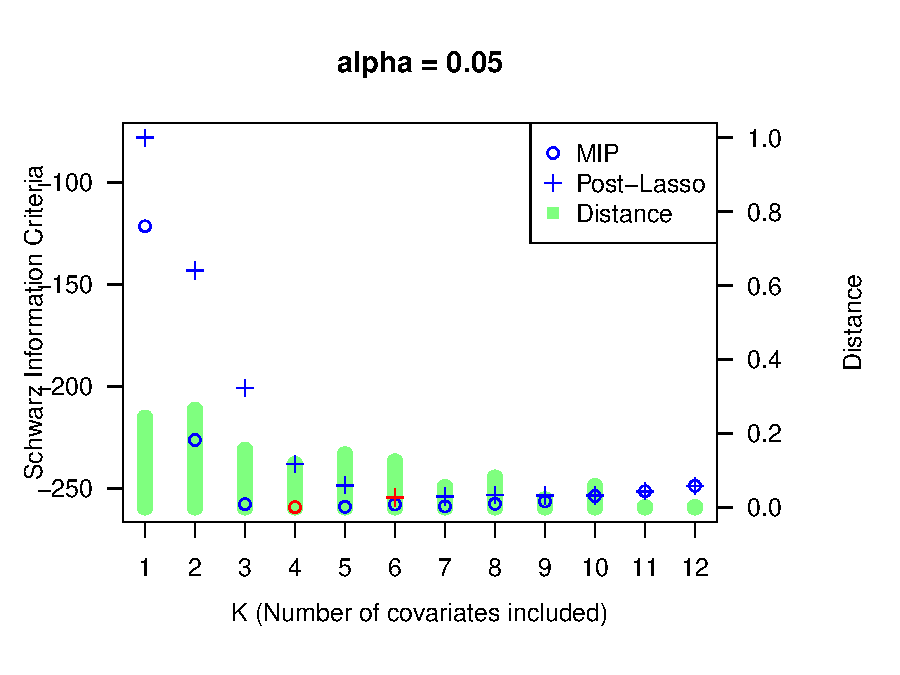
\includegraphics[width=\textwidth]{Figuras/SIC005.pdf}
    \end{minipage}
    \begin{minipage}[b]{\linewidth}
      \centering     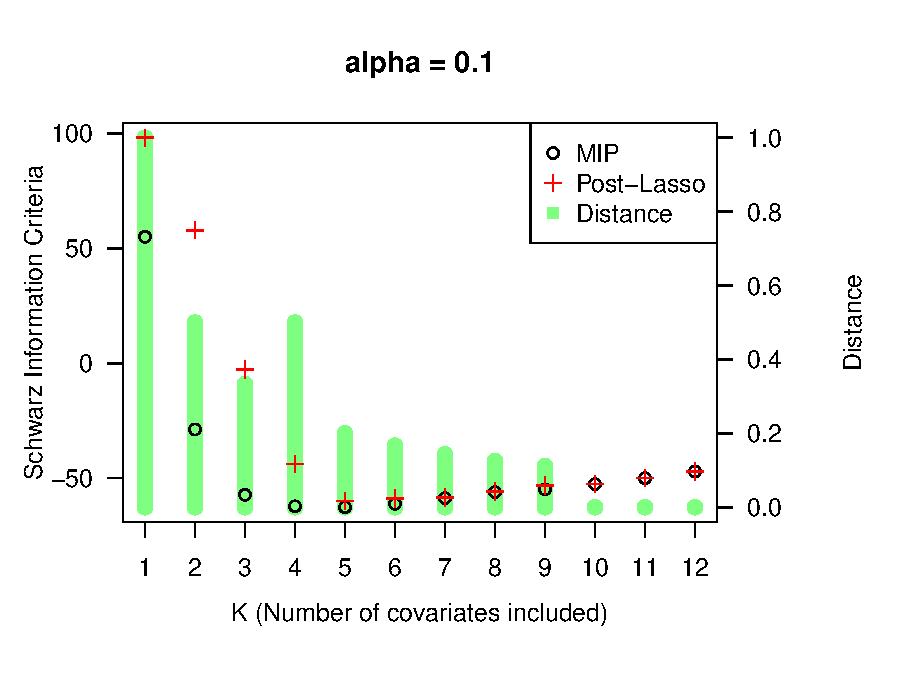
\includegraphics[width=\textwidth]{Figuras/SIC01.pdf}
    \end{minipage}
     \begin{minipage}[b]{\linewidth}
      \centering     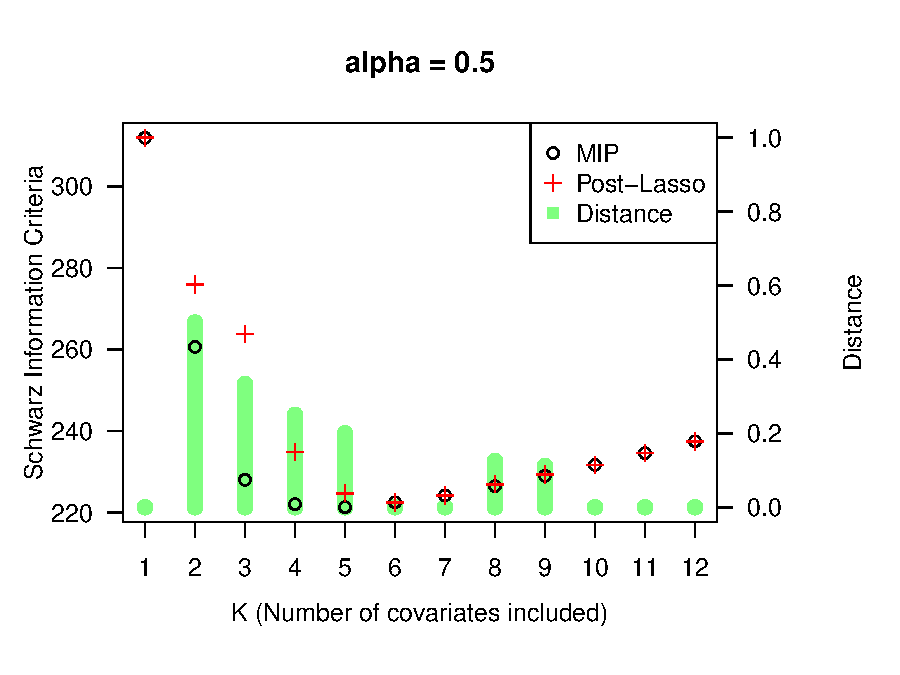
\includegraphics[width=\textwidth]{Figuras/SIC05.pdf}
     \end{minipage}
  \end{minipage}
  \begin{minipage}[t]{0.4\linewidth}
    \centering
    \begin{minipage}[b]{\linewidth}
      \centering     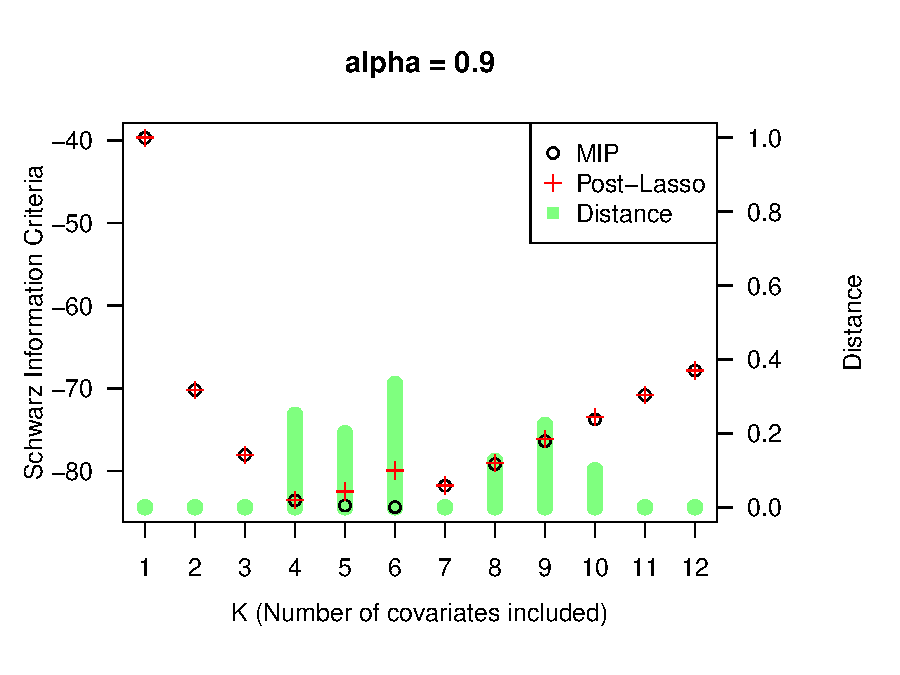
\includegraphics[width=\textwidth]{Figuras/SIC09.pdf}
    \end{minipage}
     \begin{minipage}[b]{\linewidth}
      \centering     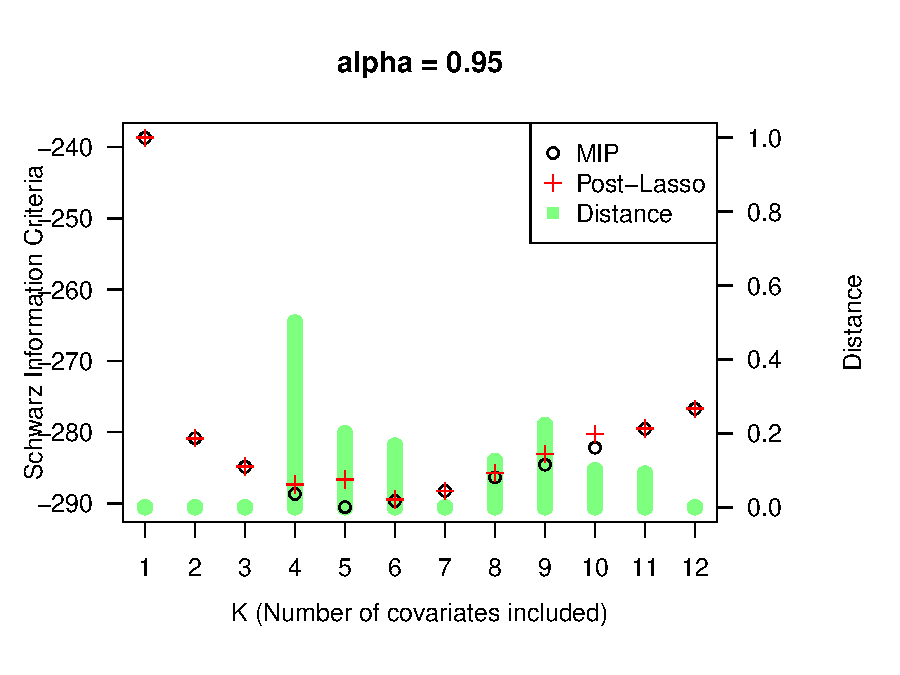
\includegraphics[width=\textwidth]{Figuras/SIC095.pdf}
      \label{fig:npqar-cross}
     \end{minipage}
  \end{minipage}
  \caption{Comparison of SIC between a solution with Lasso as a variable selector and the best subset selection with MIP. The bars represent the distance $d$ as defined by equation \ref{eq:distance}. \\ (*) When the distance is zero, it means that the same variables are selected from both methods for a given $k$. Thus, in these cases we have the same SIC for both of them.}
  \label{fig:comparison-lm-results}
\end{figure}




\subsection{Quantile Autoregression with a nonparametric approach}
\label{sec:npqar}

Fitting a linear estimator for the Quantile Auto Regression isn't appropriate  when nonlinearity is present in the data. This nonlinearity may produce a linear estimator that underestimates the quantile for a chunk of data while overestimating for the other chunk. To prevent this issue from occurring we propose a modification which we let the prediction $q_\alpha(x_t)$ adjust freely to the data and its nonlinearities. To prevent overfitting and smoothen our predictor, we include a penalty on its roughness by including the $\ell_1$ norm of its second derivative. For more information on the $\ell_1$ norm acting as a filter, one can refer to \cite{kim2009ell_1}.

This time, as opposed to when employing linear models, we don't suppose any functional form for $q_\alpha(x_t)$. This forces us to build each $q_\alpha$ differently: instead of finding a set of parameters that fully defines the function, we find a value for $q_\alpha(x_t)$ at each instant $t$. On the optimization problem, we will find optimal values for a variable $q_{\alpha t} \in \mathbb{R}$, each consisting of a single point. The sequence of $\{ q^*_{\alpha t} \} $ will provide a discretization for the full function $\hat{q}_\alpha(x_t)$, which can be found by interpolating these points.

% notação estatística de ordem. com x^(0)

Let $\{\tilde{y}_t \}_{t=1}^n$ be the sequence of observations in time $t$. Now, let $\tilde{x}_t$ be the $p-$lagged time series of $\tilde{y}_t$, such that $\tilde{x}_t = L^p(\tilde{y}_t)$, where $L$ is the lag operator. Matching each observation $\tilde{y}_t$ with its $p-$lagged correspondent $\tilde{x}_t$ will produce $n-p$ pairs $\{(\tilde{y}_t,\tilde{x}_t)\}_{t=p+1}^n$ (note that the first $p$ observations of $y_t$ must be discarded). When we order the observation of $x$ in such way that they are in growing order
$$\tilde{x}^{(p+1)} \leq \tilde{x}^{(p+2)} \leq \dots \leq \tilde{x}^{(n)},$$ 
we can then define $\{x_i\}_{i=1}^{n-p} = \{\tilde{x}^{(t)} \}_{t=p+1}^{n}$ and $\{y_i\}_{i=1}^{n-p} = \{\tilde{y}^{(t)} \}_{t=p+1}^{n}$ and $T' = \{2,\dots, n-p-1\}$. As we need the second difference of $q_i$, $I$ has to be shortened by two elements.

Our optimization model to estimate the nonparametric quantile is as follows:
\begin{equation}
\begin{split}
\hat{q}_\alpha(x_t) =\underset{q_{\alpha t}}{\arg\min}\sum_{t\in T'} \left( \alpha |y_{t}-q_{\alpha t}|^{+} + (1-\alpha)|y_{t}-q_{\alpha t}|^{-}\right) \\ +\lambda_1  \sum_{t\in T'}|D_{x_t}^{1}q_{\alpha t}| +\lambda_2  \sum_{t\in T'}|D_{x_t}^{2}q_{\alpha t}|,
\end{split}
\end{equation}
where $D^1 q_t$ and $D^2 q_t$ are the first and second derivatives of the $q_\alpha(x_t)$ function, calculated as follows:
\begin{equation*}
D_{x_{t}}^{2}q_{\alpha t}=\frac{\left(\frac{q_{\alpha t+1}-q_{\alpha t}}{x_{t+1}-x_{t}}\right)-\left(\frac{q_{\alpha t}-q_{\alpha t-1}}{x_{t}-x_{t-1}}\right)}{x_{t+1}-2x_{t} + x_{t-1}},
\end{equation*}


\begin{equation*}
D^{1}_{t \alpha }=\frac{q_{\alpha t+1}-q_{\alpha t}}{x_{t+1}-x_{t}}.
\end{equation*}
The first part on the objective function is the usual quantile regression condition for $\{q_{t\alpha}\}_{\alpha \in A}$. The second part is the $\ell_1$-filter. The purpose of a filter is to control the amount of variation for our estimator $q_\alpha(x_t)$. When no penalty is employed we would always get $q_{\alpha t} = y_t$, for any given $\alpha$. On the other hand, when $\lambda \rightarrow \infty$, our estimator approaches the linear quantile regression. 

The full model can be rewritten as a LP problem as bellow:
\begin{eqnarray}
\min_{q_{\alpha t},\delta^+_{t}, \delta_t^-, \xi_t} & \sum_{\alpha \in A} \sum_{t \in T'}\left(\alpha\delta_{t \alpha }^{+}+(1-\alpha)\delta_{t \alpha }^{-}\right) & \\
& \qquad \qquad \qquad \qquad \qquad + \lambda_1\sum_{t \in T'}\gamma_{t \alpha } + \lambda_2\sum_{t \in T'}\xi_{t \alpha } & \nonumber \\
s.t. & \delta_{t}^{+}-\delta_{t \alpha }^{-}=y_{t}-q_{t \alpha }, & \qquad\forall t \in T',\forall \alpha \in A,\\
   & D^{1}_{t \alpha }=\frac{q_{\alpha t+1}-q_{\alpha t}}{x_{t+1}-x_{t}},
    & \qquad\forall t \in T',\forall \alpha \in A,\\   
 & D^{2}_{t \alpha }=\frac{\left(\frac{q_{\alpha t+1}-q_{\alpha t}}{x_{t+1}-x_{t}}\right)-\left(\frac{q_{\alpha t}-q_{\alpha t-1}}{x_{t}-x_{t-1}}\right)}{x_{t+1}-2x_{t} + x_{t-1}}.
  & \qquad\forall t \in T',\forall \alpha \in A,\\
 & \gamma_{t \alpha}\geq D^1_{t \alpha }, & \qquad\forall t \in T',\forall \alpha \in A,\\
  & \gamma_{t \alpha}\geq-D^1_{t \alpha}, & \qquad\forall t \in T',\forall \alpha \in A,\\
  & \xi_{t \alpha}\geq D^2_{t \alpha }, & \qquad\forall t \in T',\forall \alpha \in A,\\
 & \xi_{t \alpha}\geq-D^2_{t \alpha}, & \qquad\forall t \in T',\forall \alpha \in A,\\
 & \delta_{t \alpha}^{+},\delta_{t \alpha}^{-},\gamma_{t \alpha}, \xi_{t \alpha}\geq0, & \qquad\forall t \in T',\forall \alpha \in A,\\
  & q_{t \alpha} \leq q_{t \alpha'}, & \qquad \forall t \in T', \forall (\alpha, \alpha') \in A \times A, \alpha < \alpha',\nonumber \\  
  \end{eqnarray}


The output of our optimization problem is a sequence of ordered points $\{(x_t, q_{t \alpha})\}_{t \in T}$, for all $\alpha \in A$. The next step is to interpolate these points in order to provide an estimation for any other value of $x_t$. To address this issue, we propose using a linear interpolation, that will be developed in another study. Note that $q_{t \alpha}$ is a variable that represents only one point of the $\alpha$-quantile function $q_\alpha(x_t)$. 

The quantile estimation is done for different values of $\lambda$. By using different levels of penalization on the second difference, the estimation can be more or less adaptive to the fluctuation. It is important to notice that the usage of the $\ell_1$-norm as penalty leads to a piecewise linear solution $q_{t \alpha}$. % Referenciar?
Figure \ref{fig:npqar-results} shows the quantile estimation for a few different values of $\lambda$. 

	
% Para os gráficos antigos, usar a pasta /npqar/
\begin{figure}[htp]
  \centering
  \begin{minipage}[t]{0.4\linewidth}
    \centering
    \begin{minipage}[t]{\linewidth}
      \centering     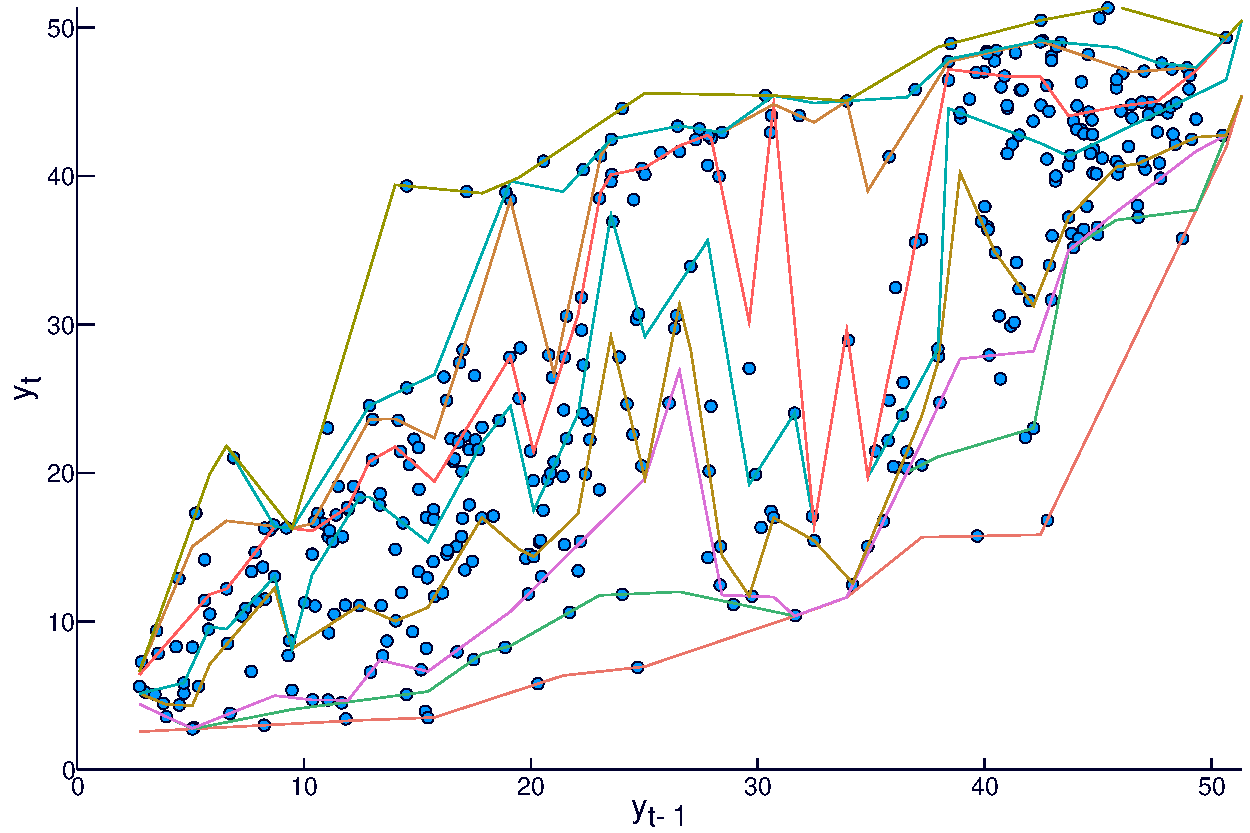
\includegraphics[width=\textwidth]{Figuras/regressao-quantilica/icaraizinho-crossing-01}
      \subcaption{$\lambda_1 = 0, \, \lambda_2 = 0.1$}
    \end{minipage}
    \begin{minipage}[b]{\linewidth}
      \centering     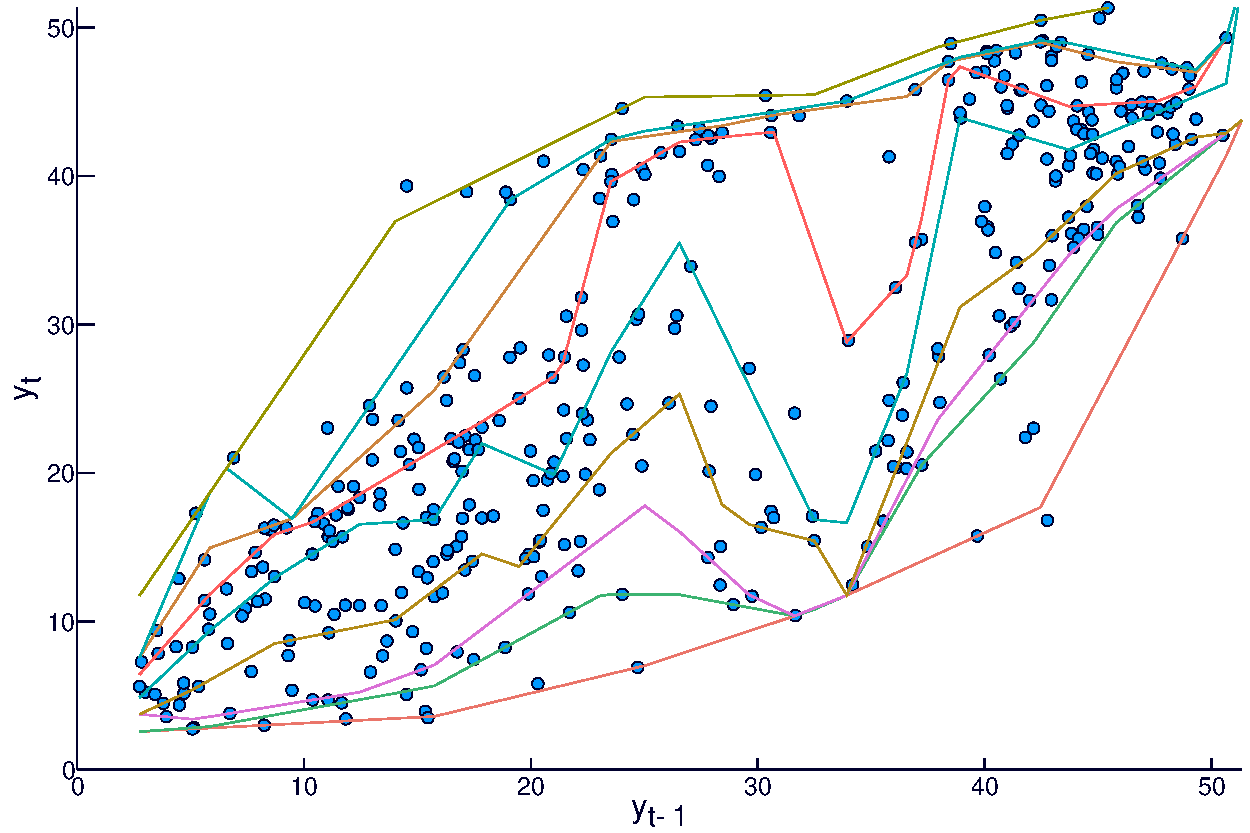
\includegraphics[width=\textwidth]{Figuras/regressao-quantilica/icaraizinho-crossing-03}
      \subcaption{$\lambda_1 = 0, \, \lambda_2 = 0.3$}
    \end{minipage}
     \begin{minipage}[b]{\linewidth}
      \centering     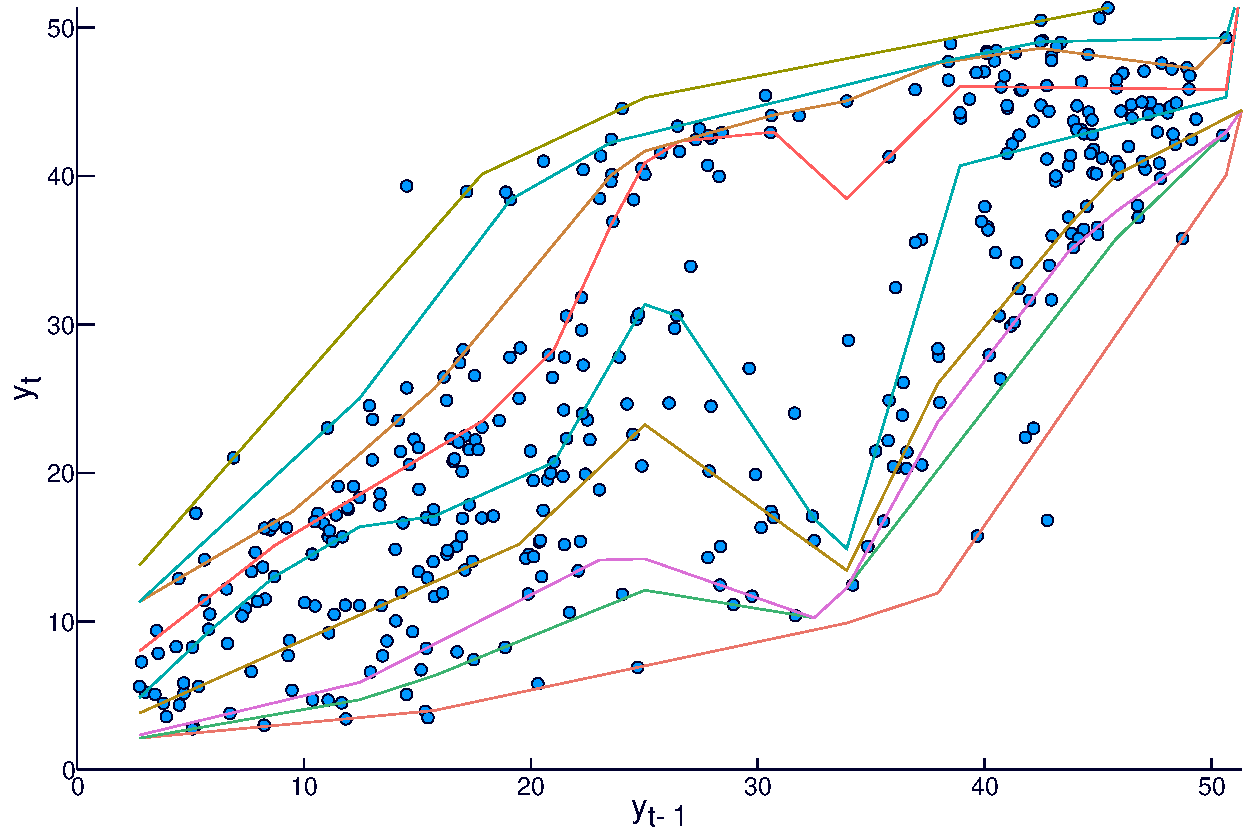
\includegraphics[width=\textwidth]{Figuras/regressao-quantilica/icaraizinho-crossing-1}
      \subcaption{$\lambda_1 = 0, \, \lambda_2 = 1$}
     \end{minipage}
  \end{minipage}
  \begin{minipage}[t]{0.4\linewidth}
    \centering
    \begin{minipage}[t]{\linewidth}
      \centering     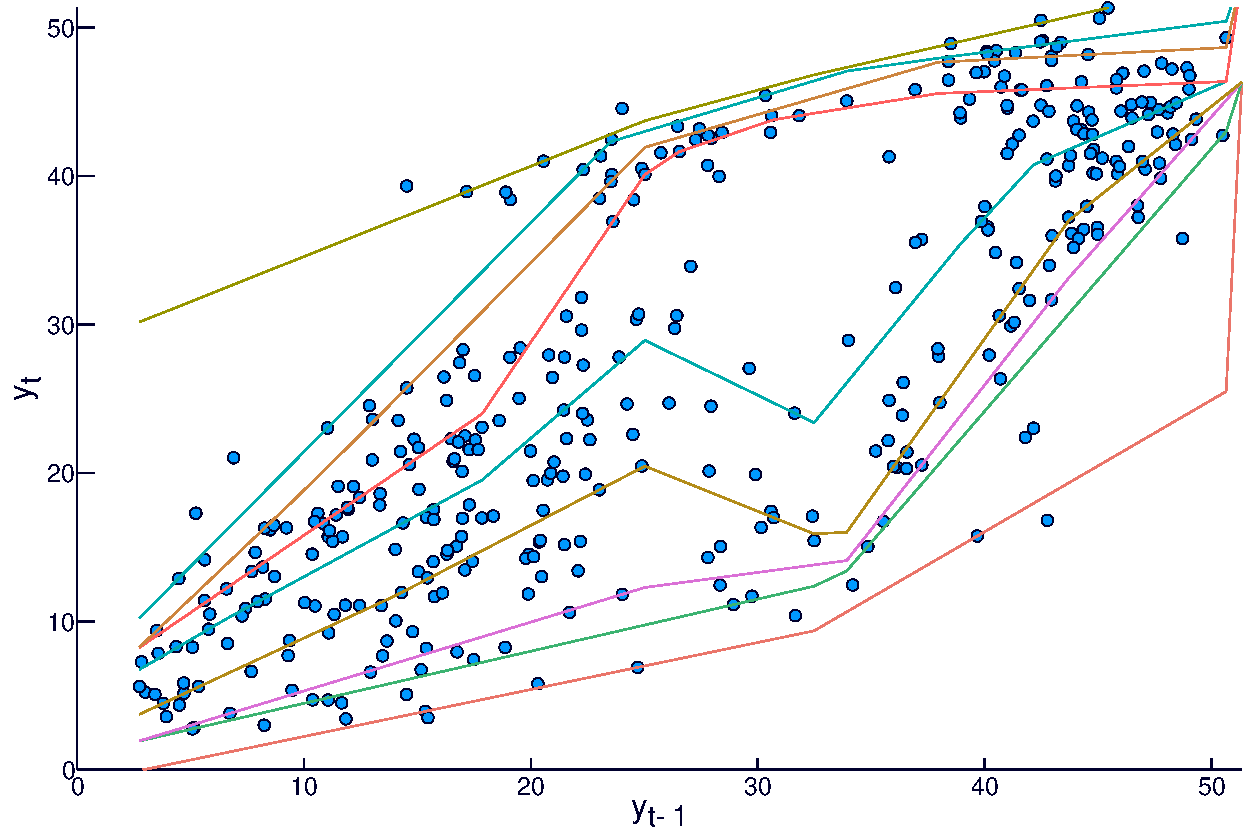
\includegraphics[width=\textwidth]{Figuras/regressao-quantilica/icaraizinho-crossing-3}
      \subcaption{$\lambda_1 = 0, \, \lambda_2 = 3$}
    \end{minipage}
    \begin{minipage}[b]{\linewidth}
      \centering     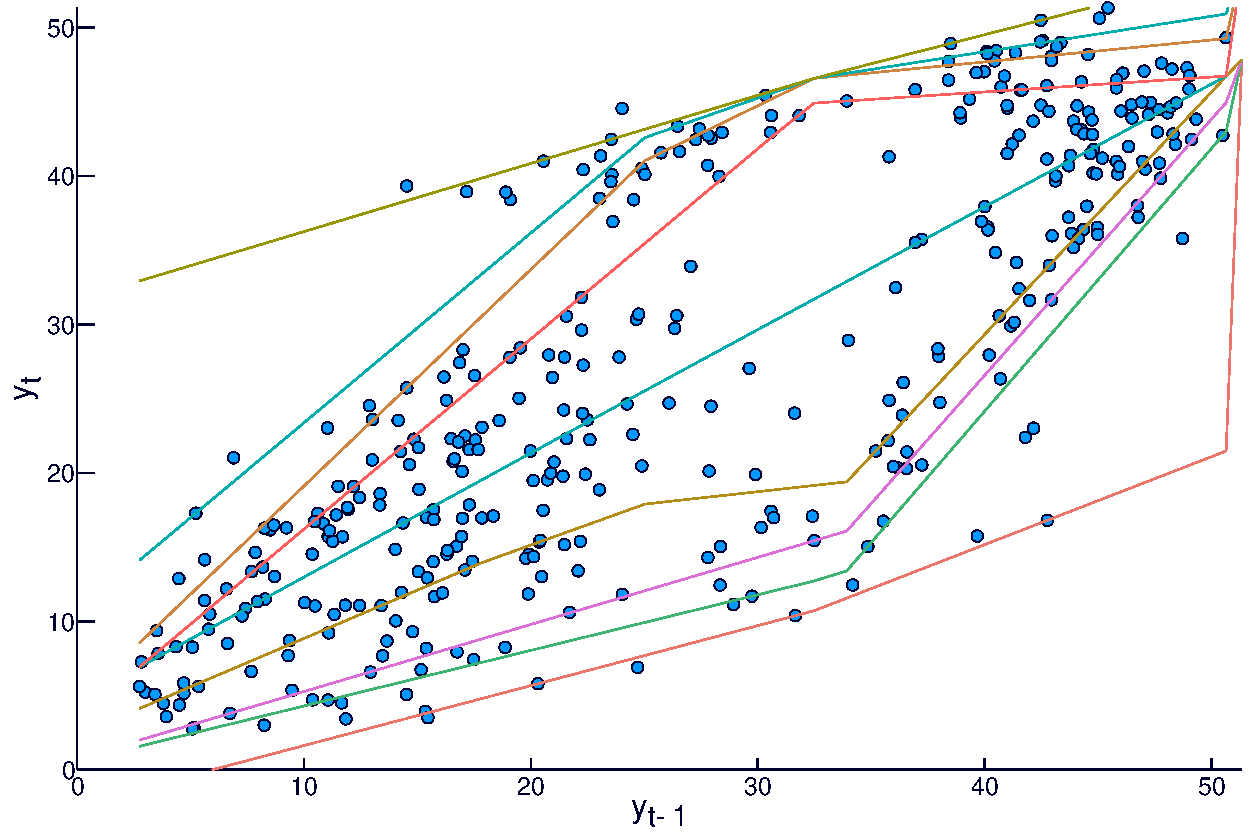
\includegraphics[width=\textwidth]{Figuras/regressao-quantilica/icaraizinho-crossing-10}
      \subcaption{$\lambda_1 = 0, \, \lambda_2 = 10$}
    \end{minipage}
     \begin{minipage}[b]{\linewidth}
      \centering     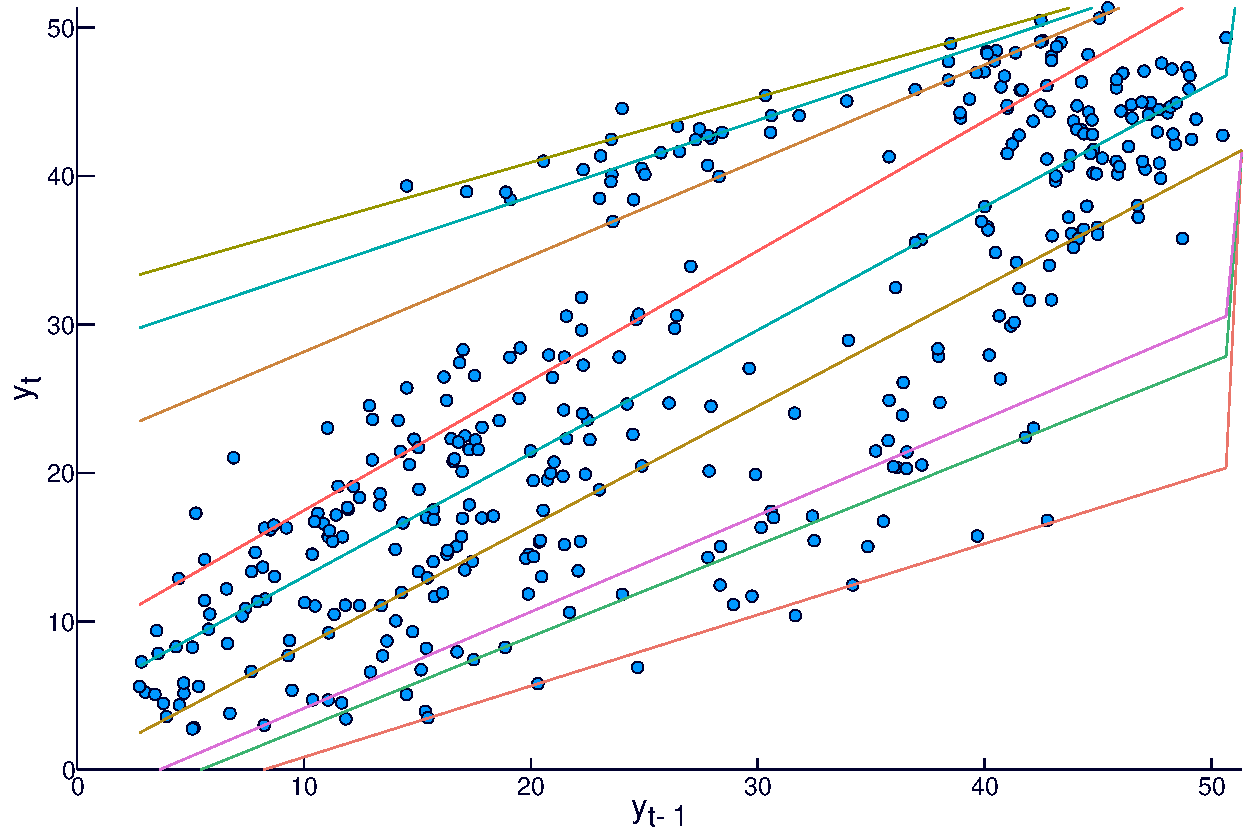
\includegraphics[width=\textwidth]{Figuras/regressao-quantilica/icaraizinho-crossing-200}
      \subcaption{$\lambda_1 = 0, \, \lambda_2 = 200$}
      \label{fig:npqar-cross}
     \end{minipage}
  \end{minipage}
  \caption{Quantile estimations for a few different values of $\lambda$. The quantiles represented here are $\alpha = (5\%, 10\%, 25\%, 50\%, 75\%, 90\%, 95\%)$. When $\lambda = 0.1$, on the upper left, we clarly see a overfitting on the estimations. The other extreme case is also shown, when $\lambda=200$ the nonparametric estimator converges to the linear model.}
  \label{fig:npqar-results}
\end{figure}

The first issue is how to select an appropriate value for $\lambda$. A simple way is to do it by inspection, which means to test many different values and pick the one that suits best our needs by looking at them. The other alternative is to use a metric to which we can select the best tune. We can achieve this by using a cross-validation method, for example.

The other issue occurs when we try to add more than one lag to the analysis at the same time. This happens because the problem solution is a set of points that we need to interpolate. This multivariate interpolation, however, is not easily solved, in the sense that we can either choose using a very naive estimator such as the K-nearest neighbors or just find another method that is not yet adopted for a wide range of applications.

%\subsection{Solar power data}
%
%While the Icaraizinho dataset has monthly observations for a wide range of time, we also test the same model for hourly data. In this case, we use the NP-QAR for solar power data. This dataset was retrieved from \textit{https://www.renewables.ninja/} and includes predicted hourly power data for the city of Tubarão (Brazil).
%This location was chosen because it is the spot of the biggest solar power plant in Brazil. 
%
%
%%Tabocas do Brejo Velho (usina solar "Horizonte" em construção, será a maior da america latina; -12.692, -44.006)
%
%
%%São José de Mipibu (usina solar  http://oportaln10.com.br/grupo-chines-instalara-fabrica-de-placas-solares-no-rn-50324/, -6.068 , -35.241)
%
%% Tubarão -28.467_-49.005_
%
%As solar power production is irradiation dependent, the best single predictor we may have is the hour of the day, as can be seen in the boxplot shown in Figure \ref{fig:solar-tubarao}
%
%\begin{figure}[h]
%	\centering
%	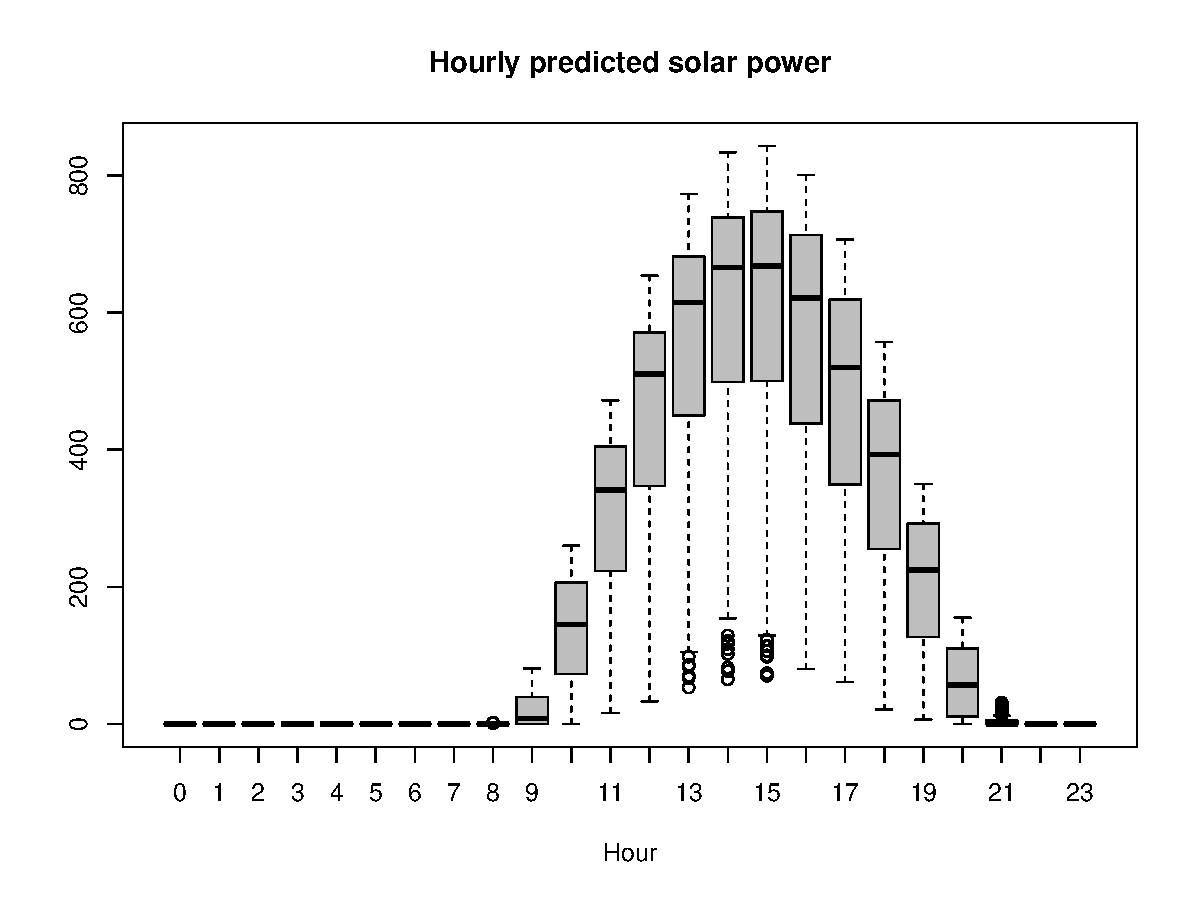
\includegraphics[width=0.8\linewidth]{Figuras/npqar-solar/hourly-solar-power.pdf}
%	\caption{Icaraizinho yearly data. Each serie consists of monthly observations for each year.}
%	\label{fig:solar-tubarao}
%\end{figure}
%
%
%
%
%
%\begin{figure}[h]
%	\centering
%		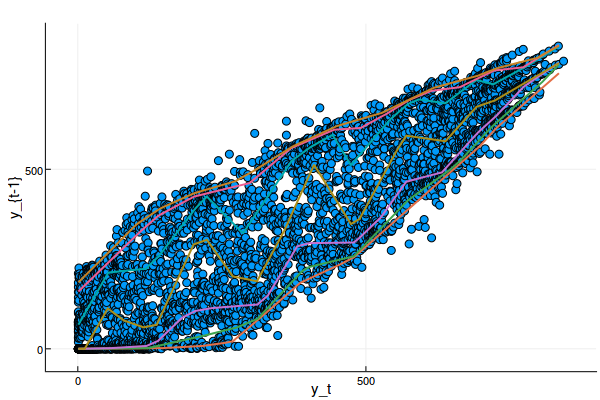
\includegraphics[width=0.8\linewidth]{Figuras/npqar-solar/com-divisao-lambda100.png}
%	\caption{Icaraizinho yearly data. Each serie consists of monthly observations for each year.}
%	\label{fig:npqar-solar-tubarao}
%\end{figure}



\subsection{A comparison between both approaches}

The last two sections introduced two different strategies to arrive in a Quantile Function $Q_{y_t|X}$. But what are the differences between using one method or the other? 

To provide a comparison between both approaches, we estimate a quantile function to predict the one-step ahead quantile function. We use as explanatory variable only the last observation $y_{t-1}$ - so $x_t = y_{t-1}$ - and estimate $\hat{q}_\alpha(y_{t-1})$, for every $\alpha \in \{0.05, 0.1, \dots, 0.9, 0.95 \}$. The result of both methods is shown on Figure \ref{fig:scatterplot-alphaquantiles}.

While the linear model produces $\alpha$-quantile functions which are linear by imposition, on the nonparametric model the $\alpha$-quantiles are flexible enough to form a hull on the data and adapt to its nonlinearities. The difference between the estimated quantile functions $\hat{Q}_{y_t|y_{t-1}}$ on both methods are shown on Figure \ref{fig:scatterplot-alphaquantiles}.

It is also important to test how the choice of the set $A$ affects the estimated quantile function. We experimented with two different sizes of $A$. In one of them, a dense grid of probabilities is used:   $A=\{0.005, 0.01, \dots, 0.99, 0.995 \}$, consisting of 199 elements. On the other only 19 elements are used to produce the quantile function ($A=\{0.05, 0.1, \dots, 0.9, 0.95 \}$).

\begin{figure}
  \centering
  \begin{minipage}[t]{\linewidth}
    \centering
    \begin{minipage}[t]{0.45\linewidth}
      \centering     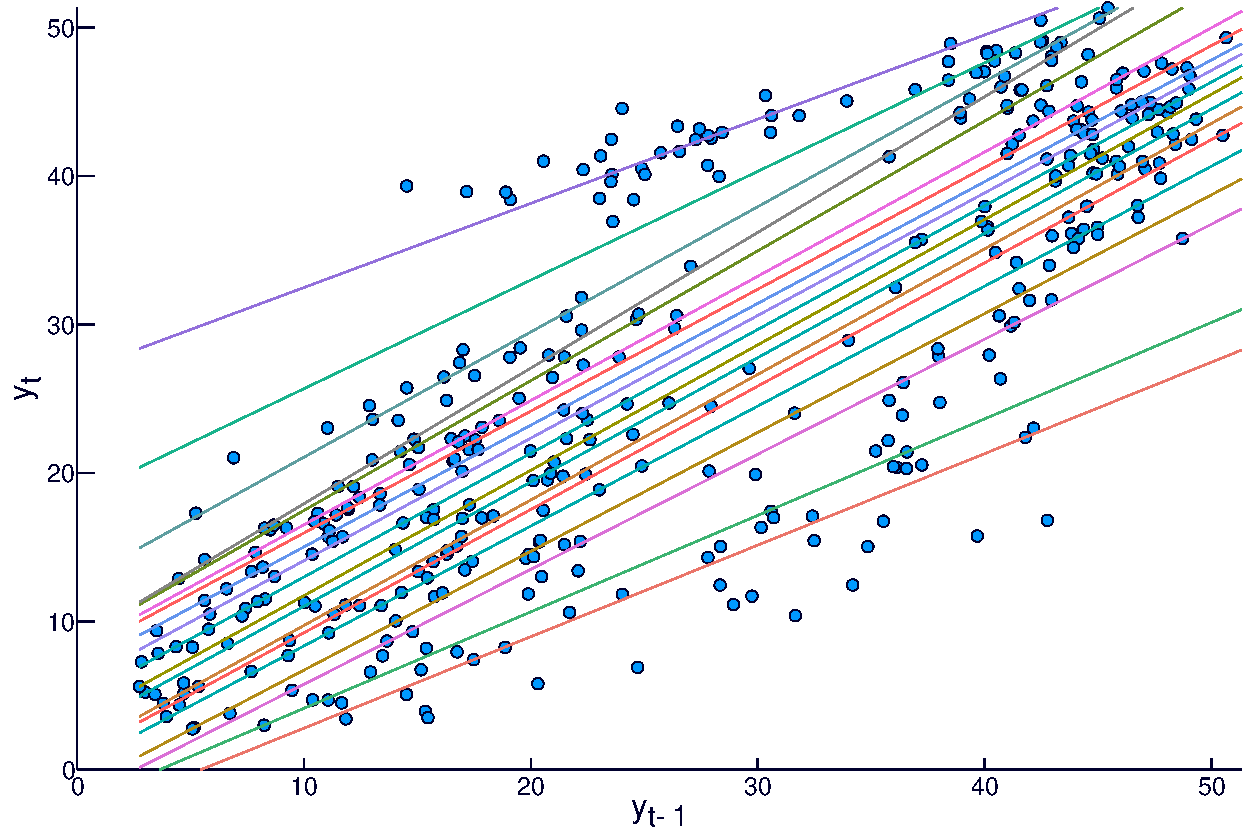
\includegraphics[width=\textwidth]{Figuras/regressao-quantilica/icaraizinho-quantile-linear-scatter}
    \end{minipage}
    \begin{minipage}[t]{0.45\linewidth}
      \centering     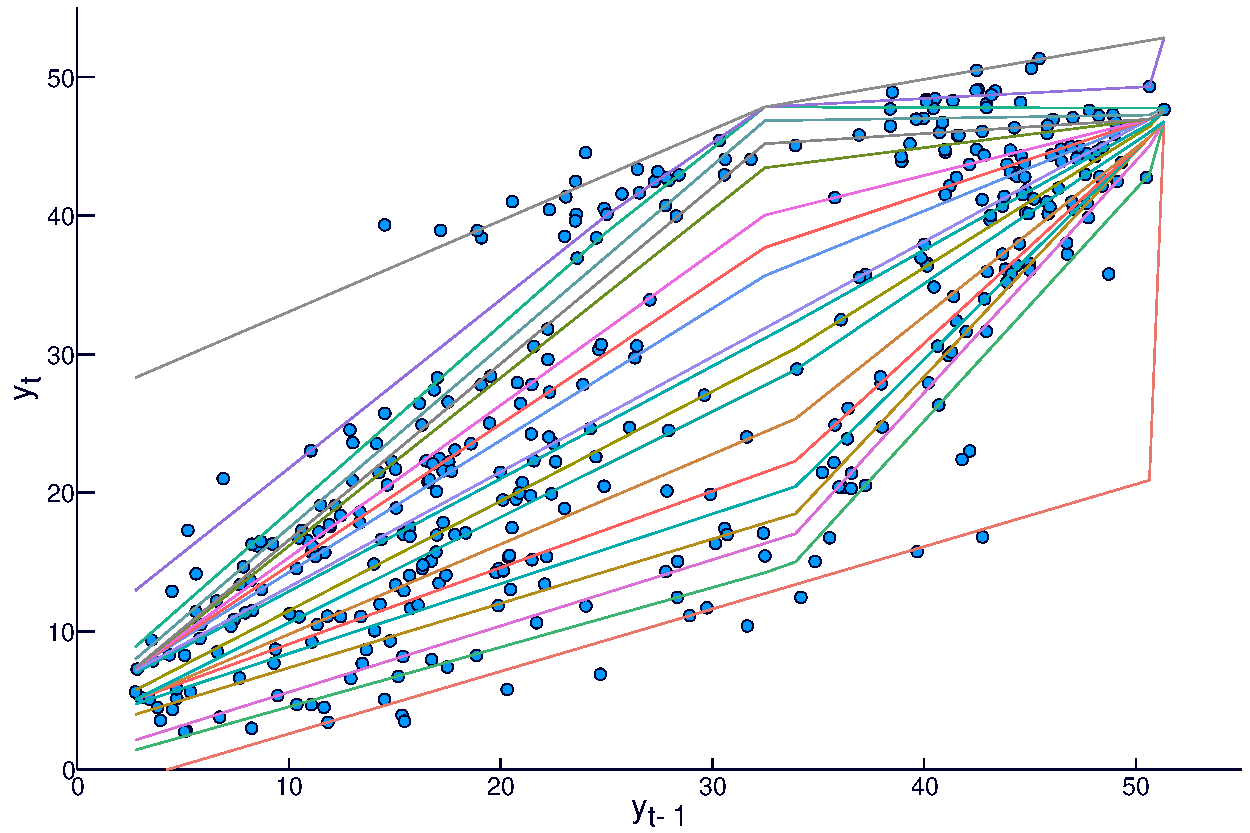
\includegraphics[width=\textwidth]{Figuras/regressao-quantilica/icaraizinho-quantile-nonpar-scatter-lambda30}
    \end{minipage}
  \end{minipage}
  \caption{Estimated $\alpha$-quantiles. On the left using a linear model and using a nonparametric approach (using $\lambda = 100$) on the right.}
  \label{fig:scatterplot-alphaquantiles}
\end{figure}




\begin{figure}
  \centering
  \begin{minipage}[t]{\linewidth}
    \centering
    \begin{minipage}[t]{0.45\linewidth}
      \centering     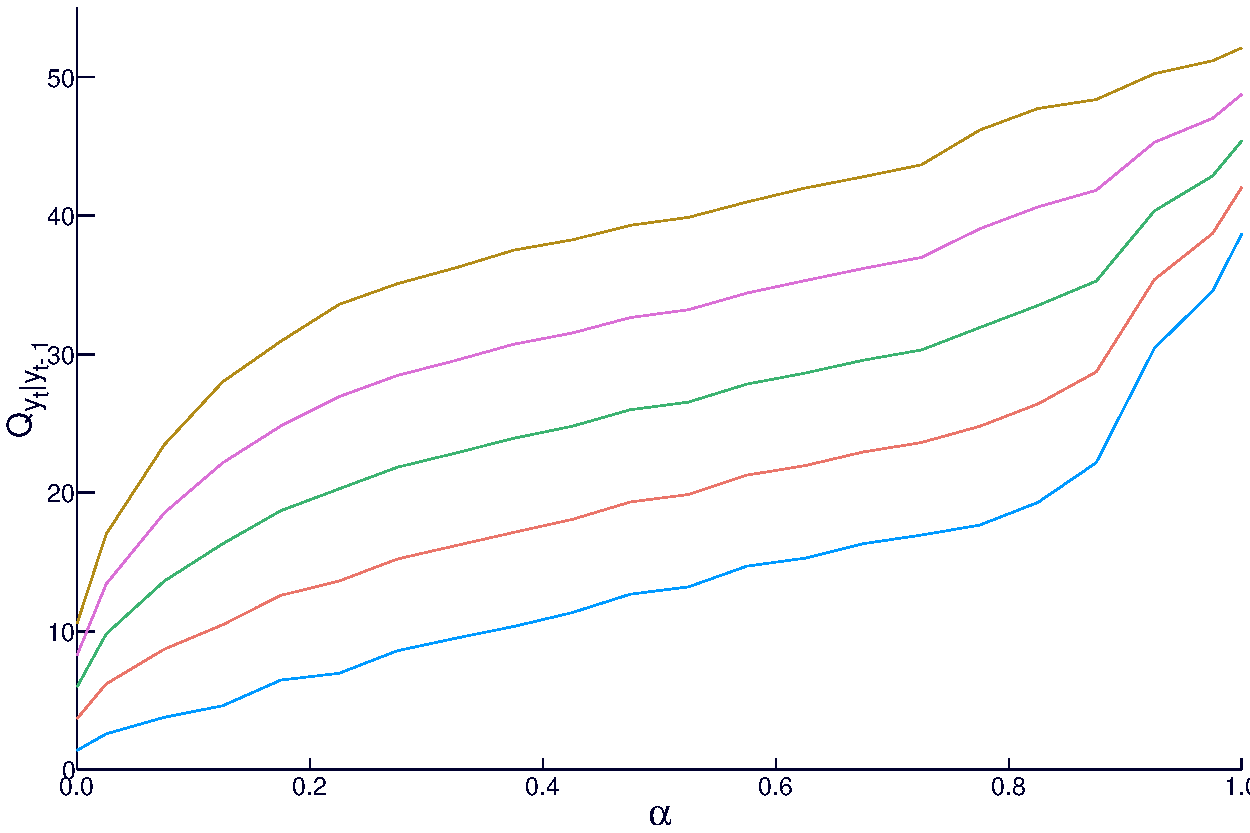
\includegraphics[width=\textwidth]{Figuras/regressao-quantilica/icaraizinho-quantile-linear}
    \end{minipage}
    \begin{minipage}[t]{0.45\linewidth}
      \centering     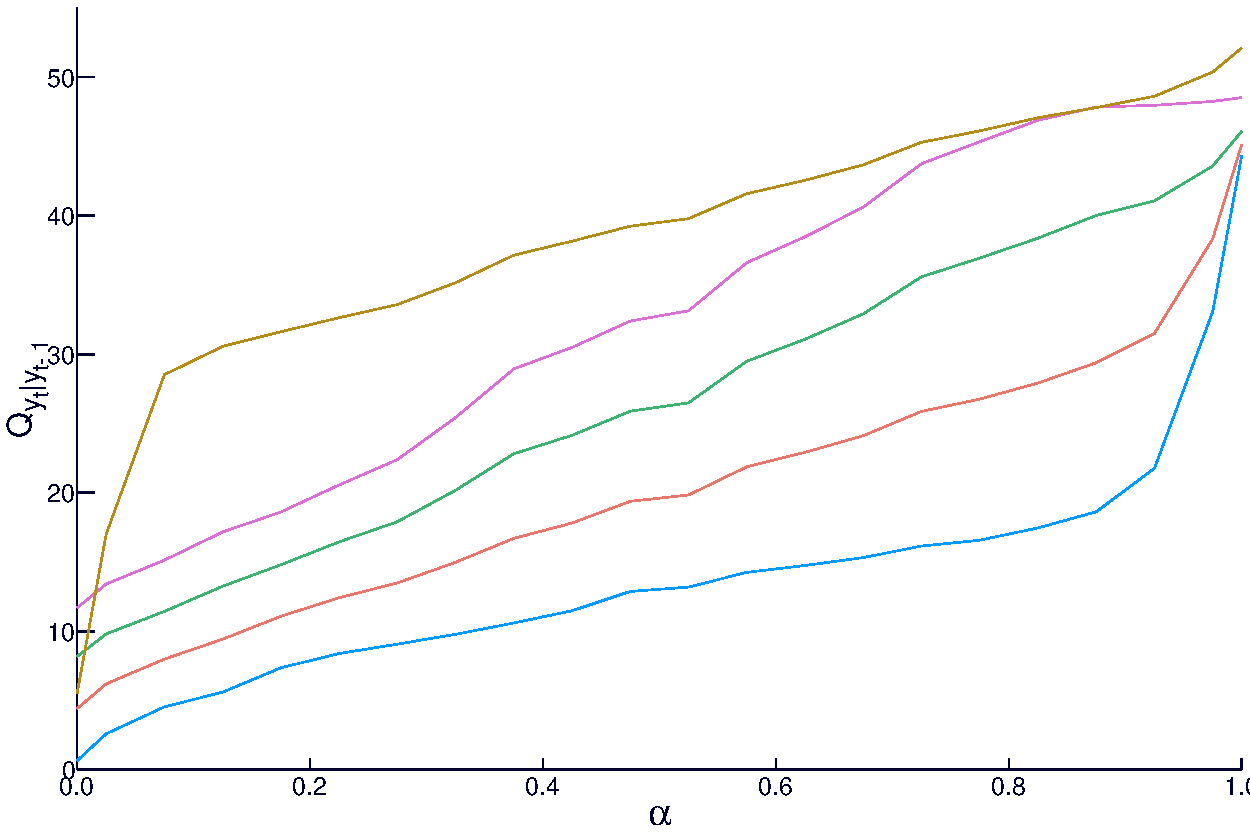
\includegraphics[width=\textwidth]{Figuras/regressao-quantilica/icaraizinho-quantile-nonpar-lambda30}
    \end{minipage}
  \end{minipage}
  \caption{Estimated quantile functions, for different values of $y_{t-1}$. On the left using a linear model and using a nonparametric approach on the right.}
  \label{fig:quantiles-vs-xt}
\end{figure}

\begin{figure}
	\centering
	\begin{minipage}[t]{\linewidth}
		\centering
		\begin{minipage}[t]{0.45\linewidth}
			\centering     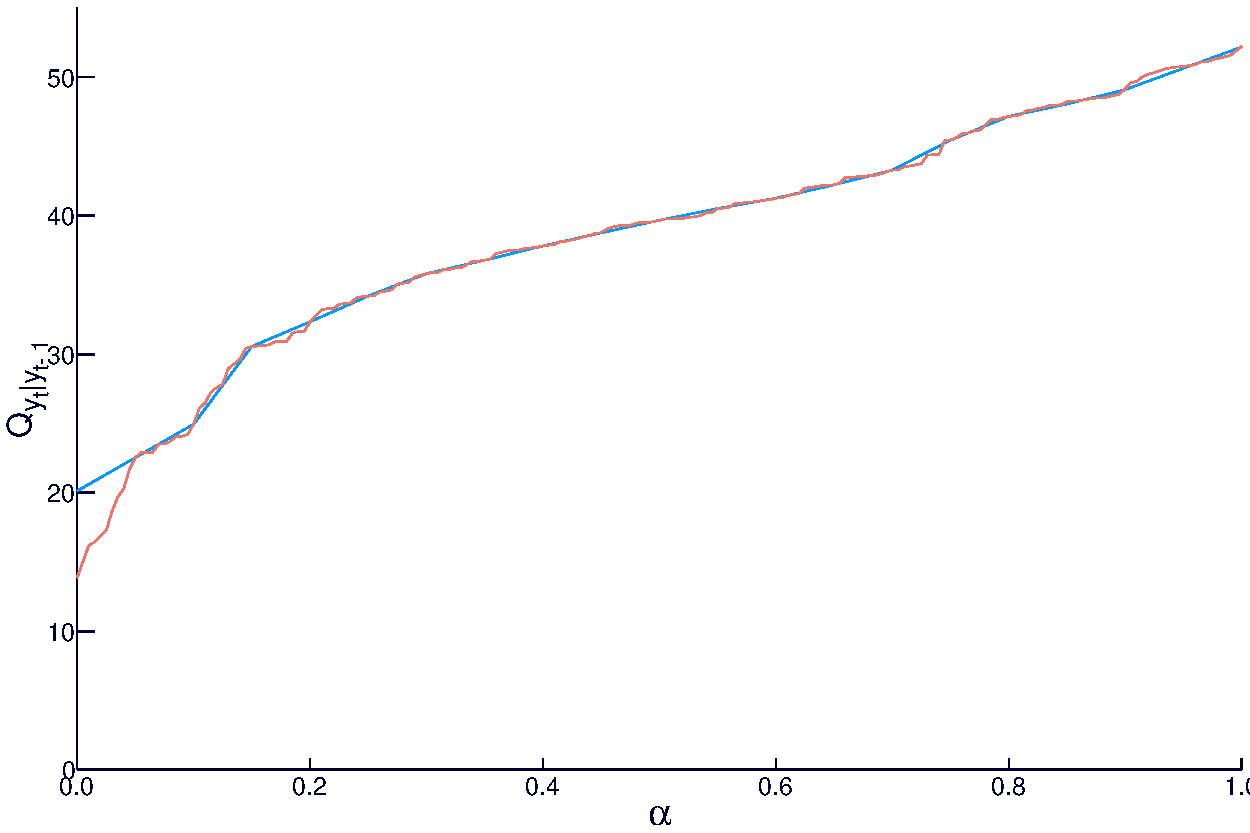
\includegraphics[width=\textwidth]{Figuras/regressao-quantilica/icaraizinho-quantile-vs-alphas-linear}
		\end{minipage}
		\begin{minipage}[t]{0.45\linewidth}
			\centering     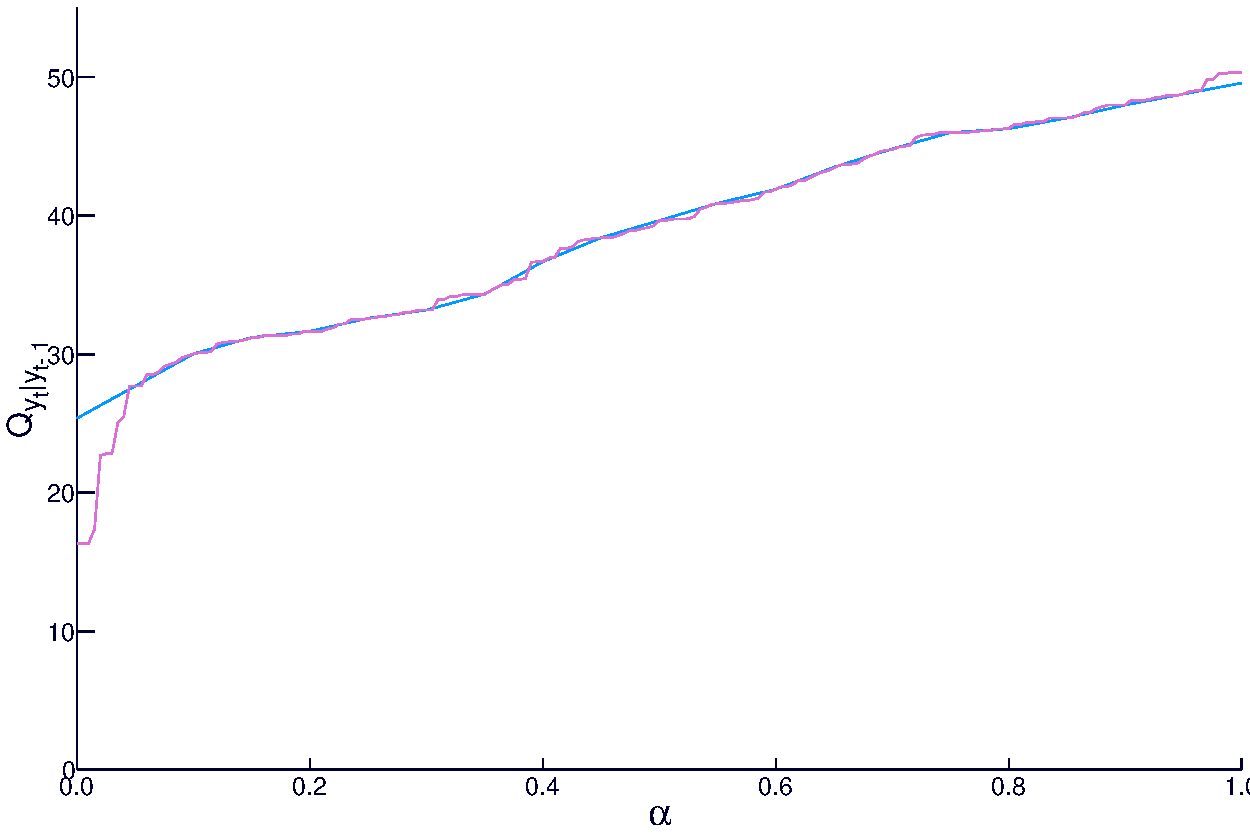
\includegraphics[width=\textwidth]{Figuras/regressao-quantilica/icaraizinho-quantile-vs-alphas-nonpar}
		\end{minipage}
	\end{minipage}
	\caption{Sensitivity to different choices of set $A$. On the left, we have the estimated quantiles for the linear model, while on the right for the nonparametric model. On both, the red line shows the quantile function estimated with $A=\{0.005, 0.01, \dots, 0.99, 0.995 \}$, consisting of 199 elements. The blue line is the estimated quantile function when $A=\{0.05, 0.1, \dots, 0.9, 0.95 \}$, consisting of only 19 elements.}
	\label{fig:quantiles-vs-xt}
\end{figure}



\subsection{Testing convergence}

In this computational exercise, we simulated the following stochastic process:
\begin{equation}
Y_t = \rho Y_{t-1}+ \varepsilon_t,\qquad \varepsilon_t \sim LogNormal(\mu,\sigma^2),
\end{equation}
to test how fast the estimated quantile function $\hat{Q}'_{Y|X}$ converges to the real $Q_{Y|X}$, using the parametric approach. An error metric defined as 
\begin{equation}
\sum_{\alpha \in A} | \hat{Q}'_{Y|X}(\alpha) - Q_{Y|X}(\alpha) |
\end{equation}
is measured for different values of size of data.
The result is shown on figure \ref{fig:convergence}.


\begin{figure}
			\centering     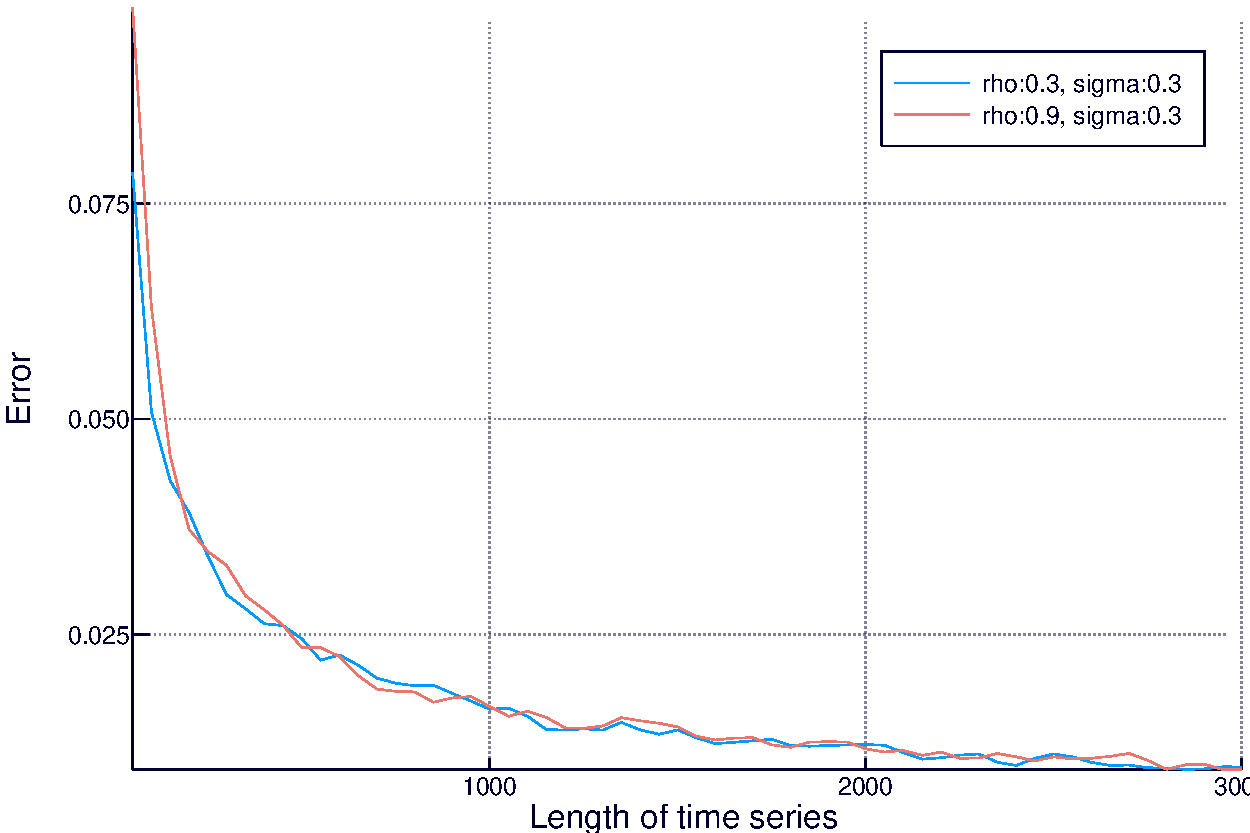
\includegraphics[width=0.6 \textwidth]{Figuras/convergencia-dist/Convergence}
	\caption{Converge of estimated quantile function to true quantile, for a LogNormal distribution}
	\label{fig:convergence}
\end{figure}
\section{Regularization}

When dealing with many candidates to use as covariates, one has to deal with the problem of selecting a subset of variables to use in constructing the model. 
This means that the vector of coefficients $\beta_\alpha = [ \beta_{1 \alpha} \cdots \beta_{P\alpha} ]$ should not have all nonzero values.
There are many ways of selecting a subset of variables among.
A classic approaches for this problem is the Stepwise algorithm \cite{efroymson1960multiple}, which includes variables in sequence. 

The approach we use in  of doing regularization and selecting the best model for estimating the quantile function. At first, we use a Mixed Integer Linear Programming optimization problem (MILP) to find the best subset among all choices of covariates. The second way is by using a LASSO-type technique, which consists in penalizing the $\ell_1$-norm of regressors, thus shrinking the size of estimated coefficients towards zero.  

\subsection{Best subset selection with MILP}
\label{sec:best-subset-mip}

In this part, we investigate the usage of MILP to select which variables are included in the model, by using a constraint which limits them to a number of $K$. This means that only $K$ coefficients $\beta_{p\alpha}$ may have nonzero values, for each $\alpha$-quantile. 
This assumption is modeled with binary variables $z_{p\alpha}$, which indicates whether $\beta_{p\alpha}$ is included or not.
The optimization problem that incorporates this idea is described below:
\begin{eqnarray}
 \underset{\beta_{0\alpha},\beta_\alpha,z_{p \alpha}, \varepsilon_{t \alpha}^{+},\varepsilon_{t \alpha}^{-}}{\text{min}} & \sum_{\alpha \in A} \sum_{t\in T}\left(\alpha\varepsilon_{t \alpha}^{+}+(1-\alpha)\varepsilon_{t\alpha}^{-}\right) \label{eq:mip0} \\
\mbox{s.t } & \varepsilon_{t \alpha}^{+}-\varepsilon_{t \alpha}^{-}=y_{t}-\beta_{0 \alpha}-\sum_{p=1}^{P}\beta_{p \alpha}x_{t,p},& \qquad\forall t \in T ,\forall \alpha \in A, \label{eq:mip1}\\
& \varepsilon_{t \alpha}^{+},\varepsilon_{t \alpha}^{-}\geq0,&\qquad\forall t \in T ,\forall \alpha \in A, \label{eq:mip2}\\
& - M z_{p \alpha} \leq \beta_{p \alpha} \leq M z_{p \alpha},&\qquad \forall \alpha \in A, \forall p\in P, \label{eq:mip3}\\
& \sum_{p=1}^P z_{p \alpha} \leq K, & \qquad \forall \alpha \in A, \label{eq:mip4}\\
& z_{p \alpha} \in \{0,1\},&\qquad \forall \alpha \in A, \forall p\in P, \label{eq:mip5}\\
& \beta_{0\alpha} + \beta_{\alpha}^T x_{t} \leq \beta_{0\alpha'} + \beta_{\alpha'}^T x_{t}, & \qquad \forall t \in T, \forall (\alpha, \alpha') \in A \times A,  \alpha < \alpha',\nonumber\\ \label{eq:mip6}
\end{eqnarray}
The objective function and constraints (\ref{eq:mip1}), (\ref{eq:mip2}) and (\ref{eq:mip6}) are those from the standard linear quantile regression. 
By constraint (\ref{eq:mip3}), variable $z_{p \alpha}$ is a binary that assumes 1 when coefficient $\beta_{p \alpha}$ is included, while (\ref{eq:mip4}) guarantees that at most $K$ of them are nonzero.
The value of $M$ is chosen in order to guarantee that $M \geq \|\hat{\beta_\alpha}\|_{\infty}$. The solution given by $\beta_{0\alpha}^*$ and $\beta_\alpha^* = [ \beta_{1 \alpha}^* \cdots \beta_{P\alpha}^* ]$ will be the best linear $\alpha$-quantile regression with $K$ nonzero coefficients.  

{
	\def\OldComma{,}
	\catcode`\,=13
	\def,{%
		\ifmmode%
		\OldComma\discretionary{}{}{}%
		\else%
		\OldComma%
		\fi%
	}%
	We ran this optimization on the Icaraizinho dataset for each value of $K \in \{0, 1, \dots, 12\}$ and quantiles $\alpha \in \{0.05, 0.1, 0.5, 0.9, 0.95\}$. The full results table can be accessed on section \ref{sec:mipcoefficients}. For all tested $\alpha$-quantiles the 12\textsuperscript{th} lag was the one included when $K=1$. 
	When $K=2$, the 1\textsuperscript{st} lag was included for all values of $\alpha$, sometimes with $\beta_{12}$, some others with $\beta_4$ and once with $\beta_{11}$. 
	These 4 lags that were present until now are the only ones selected when $K=3$. For $K=4$, those same four lags were selected for three quantiles (0.05, 0.1 and 0.5), but for the others (0.9 and 0.95) we have $\beta_6$, $\beta_7$ and $\beta_9$ also as selected. From now on, the inclusion of more lags represent a lower increase in the fit of the quantile regression. The estimated coefficient values for all $K$'s are available in the appendices section. 
}

\subsubsection*{Defining groups for variables}

Consider the optimization problem defined on (\ref{eq:mip0})-(\ref{eq:mip6}). Equation (\ref{eq:mip3}) permits a different subset of variables for each $\alpha$-quantile, as long as it is a set of $K$ variables. For two similar probabilities $\alpha$ and $\alpha'$, however, it is not plausible that their chosen model be too different (for example, in one $\beta_{1\alpha}$ and $\beta_{4\alpha}$ are selected while $\beta_{2\alpha}$ and $\beta_{5\alpha}$) are selected by the other). 

To address this issue, we propose to divide all $\alpha \in A$ into groups. The collection $G$ of all groups $g$ form a partition of $A$, and each $\alpha$ will belong to exactly one group $g$. 
The subset of selected covariates must be the same for all $\alpha$ in the same group $g$. To model these properties as constraints, we use the following equations and inequalities, that take the place of inequality \ref{eq:mip3} on the optimization problem:
\begin{eqnarray}
&z_{p \alpha g} := 2 - ( 1-z_{pg}) - I_{g\alpha}& \label{mipgrupzpa} \\
& \sum\limits_{g \in G} I_{g\alpha} = 1, & \forall \alpha \in A,\label{eq:mipgrupa} \\
& -Mz_{p \alpha g}  \leq  \beta_{p \alpha g} \leq M z_{p \alpha g}, & \forall p \in P, \quad \forall \alpha \in A, \quad \forall g \in G, \label{eq:mipgrupb} \\
& I_{g\alpha}, z_{pg} \in \{0,1\},& \forall p \in P, \quad \forall g \in G, 
\end{eqnarray}
where $G$ is a set of group index and $z_{pg}$ is a binary variable that equals 1 iff covariate $p$ is included on group $g$ and $I_{g\alpha}$ equals 1 iff probability $\alpha$ belongs to group $g$. 
The logic behind constraint \ref{eq:mipgrupb} is that 
$$\text{If }z_{pg} = 0 \text{ and }I_{g\alpha} =1 \text{ then } \beta_{p \alpha = 0}. $$
This means that if covariate $p$ belongs to group $g$, this covariate is not among group's $g$ subset of variables, than its coefficient must be equal to $0$, for that $\alpha$.
Note that variable $z_{p \alpha}$ behaves differently that when we are not considering groups. This means that if probability $\alpha$ belongs to group $g$ but variable $p$ is not selected to be among the ones of group $g$, than $\beta_{p\alpha}$ is zero.
Equation (\ref{mipgrupzpa}) defines $z_{p\alpha}$ to simplify the problem.

\todo[inline]{Colocar resultados dos experimentos MILP-Grupos vs. MILP depois de concluídos. Se resultados de grupos com rampa forem bons, incluír aqui mais uma seção.}
%
%\subsubsection*{Defining groups for variables where each group consists of probabilities in sequence}
%%
%Each groups $g \in G$, as defined on the last section, may be any combination of probabilities $\alpha$, such that they don't be in sequence. Figure \ref{fig:heatmap-exemplo-grupos} shows an example of 
%
%\begin{figure}
%	\centering
%	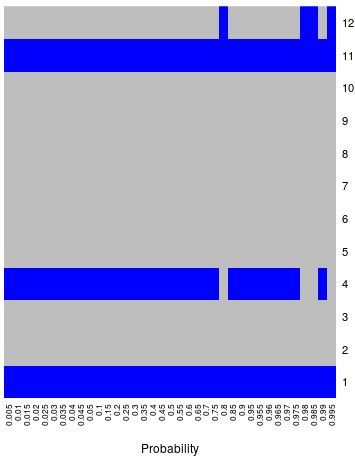
\includegraphics[width=0.4\linewidth]{Figuras/betas-mip/heatmap-exemplo-grupos}
%	\caption{}
%	\label{fig:heatmap-exemplo-grupos}
%\end{figure}
%
%
%\begin{eqnarray}
%\underset{\beta_{0\alpha},\beta_\alpha,z_{p \alpha}, \phi_{p \alpha}, \varepsilon_{t \alpha}^{+},\varepsilon_{t \alpha}^{-}}{\text{min}} & \sum_{\alpha \in A} \sum_{t\in T}\left(\alpha\varepsilon_{t \alpha}^{+}+(1-\alpha)\varepsilon_{t\alpha}^{-}\right) \label{eq:mipgr0} \\
%\mbox{s.t } & \varepsilon_{t \alpha}^{+}-\varepsilon_{t \alpha}^{-}=y_{t}-\beta_{0 \alpha}-\sum_{p=1}^{P}\beta_{p \alpha}x_{t,p},& \qquad\forall t \in T ,\forall \alpha \in A, \label{eq:mipgr1}\\
%& \varepsilon_{t \alpha}^{+},\varepsilon_{t \alpha}^{-}\geq0,&\qquad\forall t \in T ,\forall \alpha \in A, \label{eq:mipgr2}\\
%& - M z_{p \alpha} \leq \beta_{p \alpha} \leq M z_{p \alpha},&\qquad \forall \alpha \in A, \forall p\in\{1,\dots,P\}, \label{eq:mipgr3}\\
%& \sum_{p=1}^P z_{p \alpha} \leq K, & \qquad \forall \alpha \in A, \label{eq:mipgr4}\\
%& z_{p \alpha} \in \{0,1\},&\qquad \forall \alpha \in A, \forall p\in\{1,\dots,P\}, \label{eq:mipgr5}\\
%& \beta_{0\alpha} + \beta_{\alpha}^T x_{t} \leq \beta_{0\alpha'} + \beta_{\alpha'}^T x_{t}, & \qquad \forall t \in T, \forall (\alpha, \alpha') \in A \times A,  \alpha < \alpha',\nonumber\\ \label{eq:mipgr6} \\
%& z_{p\alpha} - z_{p\alpha+1} \leq m_{p\alpha}, & \qquad \forall \alpha \in A', \qquad \forall p \in P  \\
%& \sum_{\alpha \in A'} r_\alpha \leq |G| - 1 
%\label{eq:mipgr} \\
%\end{eqnarray}
%where $A' = A\setminus \{|A|\}$

\subsection{Best subset selection with LASSO}
\label{sec:best-subset-ell1}

Another way of doing regularization is including the $\ell_1$-norm of the coefficients on the objective function. The advantage of this method is that coefficients are shrunk towards zero by changing a continuous parameter $\lambda$, which penalizes the size of the $\ell_1$-norm.  
When the value of $\lambda$ gets bigger, fewer variables are selected to be used. 
This is the same strategy of the LASSO methodology, and its usage for the quantile regression is discussed in \cite{li2012l1}.
The proposed optimization problem to be solved is:
\begin{equation}
\underset{\beta_{0\alpha},\beta_\alpha}{\text{min}} \sum_{t \in T}\alpha|y_{t}-q_\alpha(x_t)|^{+}+ \sum_{t \in T}(1-\alpha)|y_{t}-q_\alpha(x_t)|^{-}+\lambda\|\beta_\alpha\|_{1},
\label{eq:l1-qar-optim}
\end{equation}
\[
q_\alpha(x_t)=\beta_{0}-\sum_{p=1}^{P}\beta_{p}x_{t,p}.
\]

For such estimation to be coherent, however, each covariate must have the same relative weight in comparison with one another. 
So, before solving the optimization problem, we perform a linear transformation such that all variables have mean $\mu = 0$ and variance $\sigma^2 = 1$. 
We apply the transformation $\tilde{x}_{t,p} = (x_{t,p} - \bar{x}_{t,p}) / \hat\sigma_{x_{t,p}}$, where $\bar{x}_{t,p}$ and $\hat{\sigma}_{x_{t,p}}$ are respectively the sample's unconditional mean and standard deviation. The $\tilde{y}_{t-p,i}$ series will be used to estimate the coefficients, as this series has the desired properties. 

After the process of normalization, we can rewrite problem \ref{eq:l1-qar-optim} as a LP problem, as shown below:
\begin{eqnarray}
\tilde \beta_\lambda^{*LASSO} = \underset{\beta_{0},\beta,\varepsilon_{t \alpha}^{+},\varepsilon_{t \alpha}^{-}}{\text{arg min}} & \sum_{\alpha \in A} \sum_{t \in T}\left(\alpha\varepsilon_{t \alpha}^{+}+(1-\alpha)\varepsilon_{t \alpha}^{-}\right)+\lambda\sum_{p=1}^{P}\mbox{\ensuremath{\xi}}_{p \alpha} \label{eq:obj-lasso} \\
\mbox{s.t. } & \varepsilon_{t \alpha}^{+}-\varepsilon_{t \alpha}^{-}= y_{t}-\beta_{0 \alpha}-\sum_{p=1}^{P}\beta_{p \alpha}\tilde x_{t,p},&\forall t\in T, \forall \alpha \in A, \\
& \varepsilon_{t \alpha}^{+},\varepsilon_{t \alpha}^{-}\geq0,&\forall t \in T, \forall \alpha \in A,\\
& \xi_{p\alpha}\geq\beta_{p \alpha},&\forall p\in P, \forall \alpha \in A,  \label{l1-qar-3}
\\
& \xi_{p\alpha}\geq-\beta_{p \alpha},&\forall p\in P, \forall \alpha \in A.  \label{l1-qar-4}
\end{eqnarray}
This model is built upon the standard linear programming model for the quantile regression (\ref{eq:linear-opt-1})-(\ref{eq:linear-opt-ult}). 
On the above formulation, the $\ell_1$ norm of equation (\ref{eq:l1-qar-optim}) is substituted by the sum of $\xi_p$, which represents the absolute value of $\beta_{p\alpha}$. The link between variables $\xi_p$ and $\beta_{p\alpha}$ is made by constraints (\ref{l1-qar-3}) and (\ref{l1-qar-4}). Note that the linear coefficient $\beta_{0\alpha}$ is not included in the penalization, as the sum of penalties on the objective function \ref{eq:obj-lasso}.

% % % % % % % % Esse trecho deve ser usado quando os coeficientes do lasso forem utilizados, e não apenas o lasso sendo um seletor de variáveis % % % % % % % % %
%Each component of the output $\tilde \beta_\lambda^{*LASSO}$ must be corrected by multiplying each coefficient for its standard deviation: $\beta_{p\alpha,\lambda}^{*LASSO} = \tilde \beta_{p\alpha,\lambda}^{*LASSO} \hat\sigma_{x_{t,p}}$.
%\begin{eqnarray}
%\tilde \beta_\lambda^{*LASSO} = \underset{\beta_{0},\beta,\varepsilon_{t \alpha}^{+},\varepsilon_{t \alpha}^{-}}{\text{arg min}} & \sum_{\alpha \in A} \sum_{t \in T}\left(\alpha\varepsilon_{t \alpha}^{+}+(1-\alpha)\varepsilon_{t \alpha}^{-}\right)+\lambda\sum_{p=1}^{P}\mbox{\ensuremath{\xi}}_{p \alpha} \label{eq:obj-lasso} \\
%\mbox{s.t. } & \varepsilon_{t \alpha}^{+}-\varepsilon_{t \alpha}^{-}= y_{t}-\beta_{0 \alpha}-\sum_{p=1}^{P}\beta_{p \alpha}\tilde x_{t,p},&\forall t\in T, \forall \alpha \in A, \\
%& \varepsilon_{t \alpha}^{+},\varepsilon_{t \alpha}^{-}\geq0,&\forall t \in T, \forall \alpha \in A,\\
%& \xi_{p\alpha}\geq\beta_{p \alpha},&\forall p\in P, \forall \alpha \in A,  \label{l1-qar-3}
%\\
%& \xi_{p\alpha}\geq-\beta_{p \alpha},&\forall p\in P, \forall \alpha \in A.  \label{l1-qar-4}
%\end{eqnarray}



For low values of $\lambda$, the penalty over the size of coefficients is small. Because of that, the output of problem (\ref{eq:obj-lasso})-(\ref{l1-qar-4}) is a model where most coefficients have nonzero value. On the other hand, when the penalty on $\| \beta_\alpha \|_1$ is big, many covariates will have zero valued coefficients. When $\lambda$ approaches infinity, one has a constant model. 
For instance, the penalty isn't applied to the linear coefficient $\beta_{0\alpha}$. 

Even though we have coefficients that are estimated by this method, we don't use them directly. In fact, the LASSO coefficients are biased, so it is employed only as a variable selector. As so, the nonzero coefficient covariates will be the input of a unrestricted quantile regression problem, as in the linear programming problem (\ref{eq:linear-opt-1})-(\ref{eq:linear-opt-ult}). 
The set of selected indexes are given by
\begin{equation*}
L_\lambda = \{ p \in \{ 1,\dots,P \} | \; |\beta^{*LASSO}_{\lambda,p}| \neq 0  \}.
\end{equation*}
Hence, we have that, for each $p \in \{ 1,\dots,P \}$,
$$\beta^{*LASSO}_{\lambda,p} = 0 \Longrightarrow \beta^{*}_{\lambda,p} = 0.$$
The post-lasso coefficients $\beta_\lambda^*$ are the solution from the optimization problem given below:
\begin{equation}
\begin{aligned} (obj_{\lambda}^{*},\beta_{\lambda}^{*})\overset{(obj,var)}{\longleftarrow} \min_{\beta_0,\beta,\varepsilon_{t}^{+},\varepsilon_{t}^{-}} & \sum_{t \in T}\left(\alpha\varepsilon_{t}^{+}+(1-\alpha)\varepsilon_{t}^{-}\right) \\
\mbox{s.t. } & \varepsilon_{t}^{+}-\varepsilon_{t}^{-}=y_{t} - \beta_0 - \sum_{p\in L_\lambda} \beta_p x_{t,p},& \forall t\in T,\\
& \varepsilon_t^+,\varepsilon_t^- \geq 0, & \forall t \in T.
\end{aligned}
\label{eq:post-lasso}
\end{equation}
The variable $obj_{\lambda}^{*}$ receives the value of the objective function on its optimal solution.
In summary, the optimization in equation \ref{eq:l1-qar-optim} acts as a variable selection for the subsequent estimation, which is normally called the post-LASSO estimation \cite{belloni2009least}.


For the same quantile values, $\alpha$, we experimented on section \ref{sec:best-subset-mip} ($\alpha \in \{0.05, 0.1, 0.5, 0.9, 0.95\}$), we estimate the post-LASSO (from now on, we call it just LASSO, for simplicity). Figure \ref{fig:lasso-results} shows the path of variables for each $\alpha$-quantile. On the x-axis, we have the penalty $\lambda$ in a log scale. On the y-axis we have the size of coefficients. One can see how increasing $\lambda$ leads to a shrinking on the size of coefficients, up to a point where all coefficients are equal to 0.
\begin{figure}
	\centering
	\begin{minipage}[t]{0.4\linewidth}
		\centering
		\begin{minipage}[t]{\linewidth}
			\centering     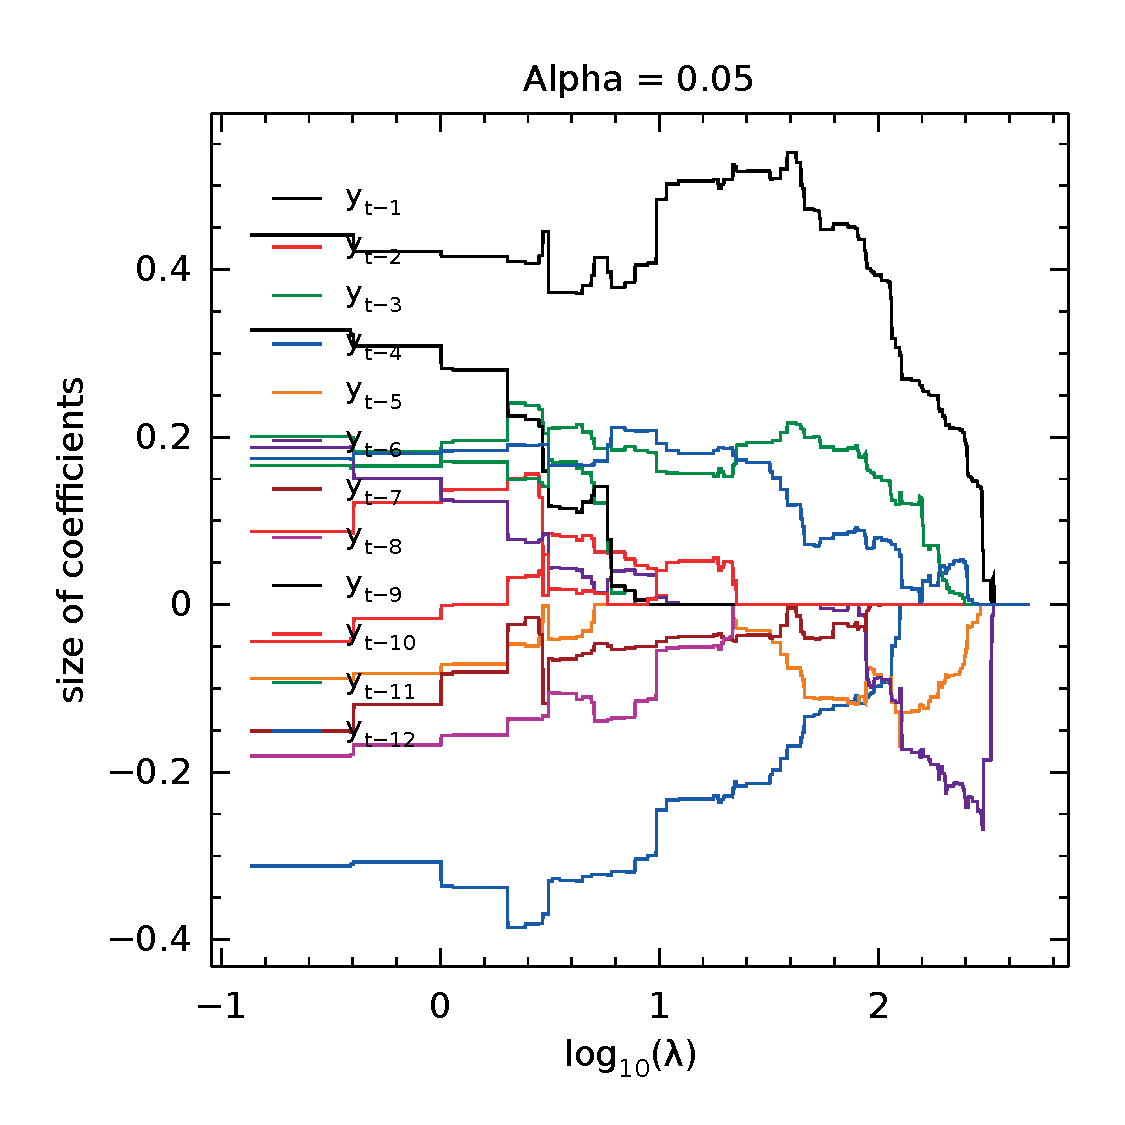
\includegraphics[width=\textwidth]{Figuras/selecao-lasso/par-sellasso-005.pdf}
		\end{minipage}
		\begin{minipage}[b]{\linewidth}
			\centering     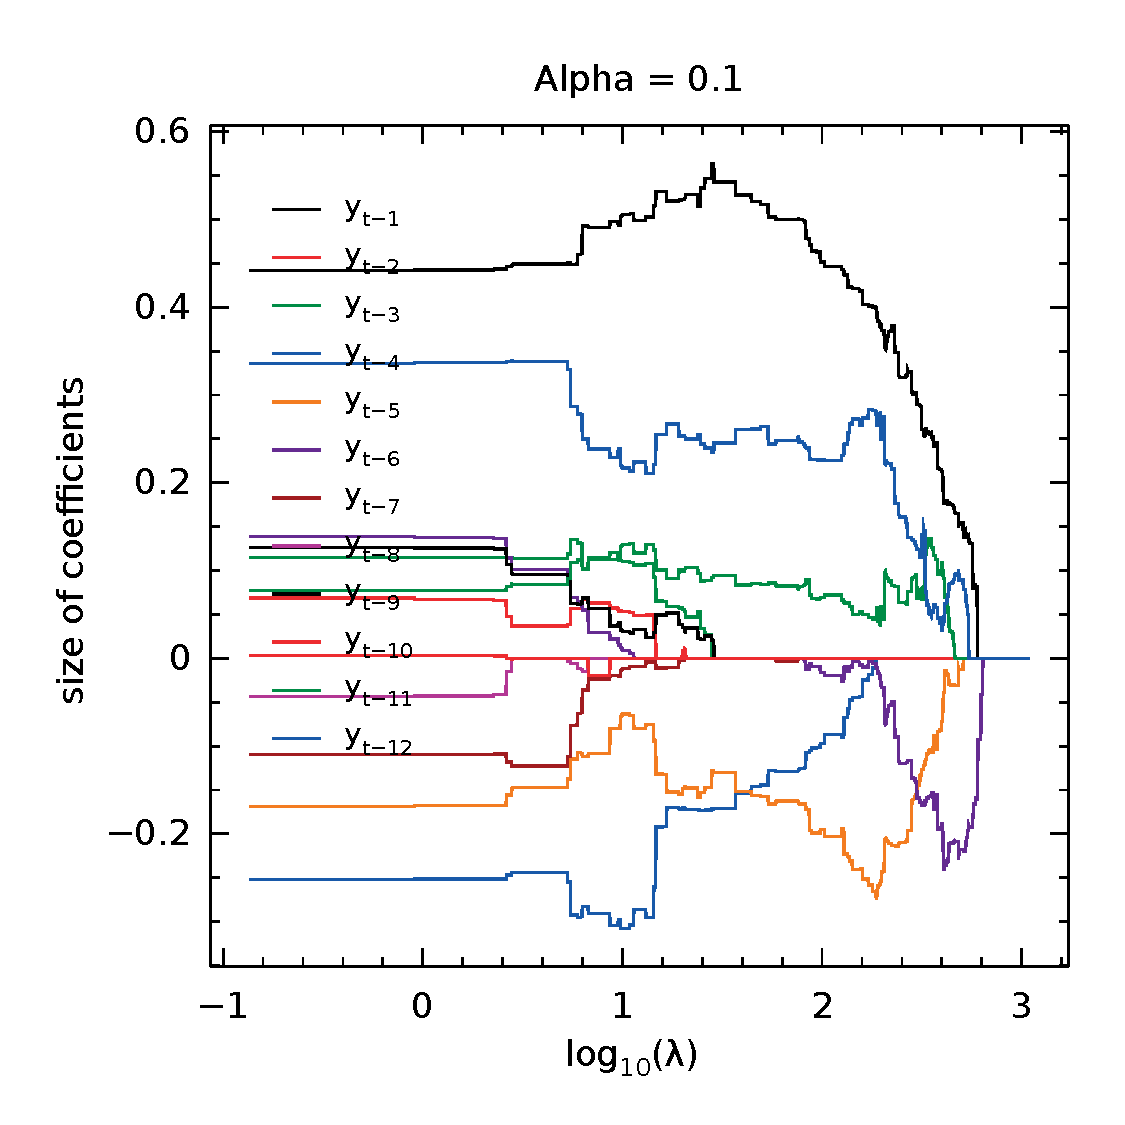
\includegraphics[width=\textwidth]{Figuras/selecao-lasso/par-sellasso-01.pdf}
		\end{minipage}
		\begin{minipage}[b]{\linewidth}
			\centering     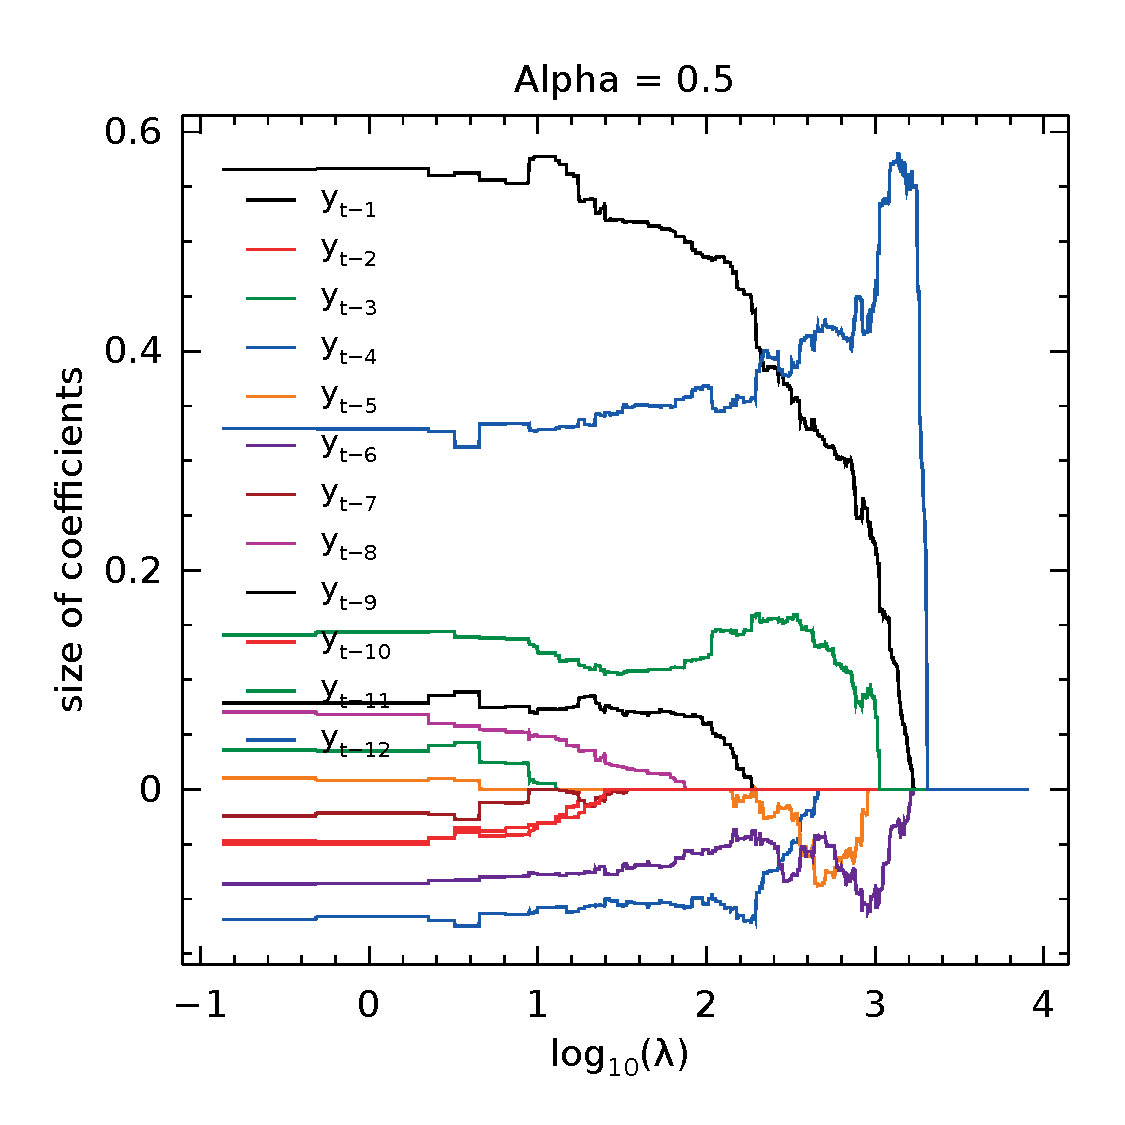
\includegraphics[width=\textwidth]{Figuras/selecao-lasso/par-sellasso-05.pdf}
		\end{minipage}
	\end{minipage}
	\begin{minipage}[t]{0.4\linewidth}
		\centering
		\begin{minipage}[b]{\linewidth}
			\centering     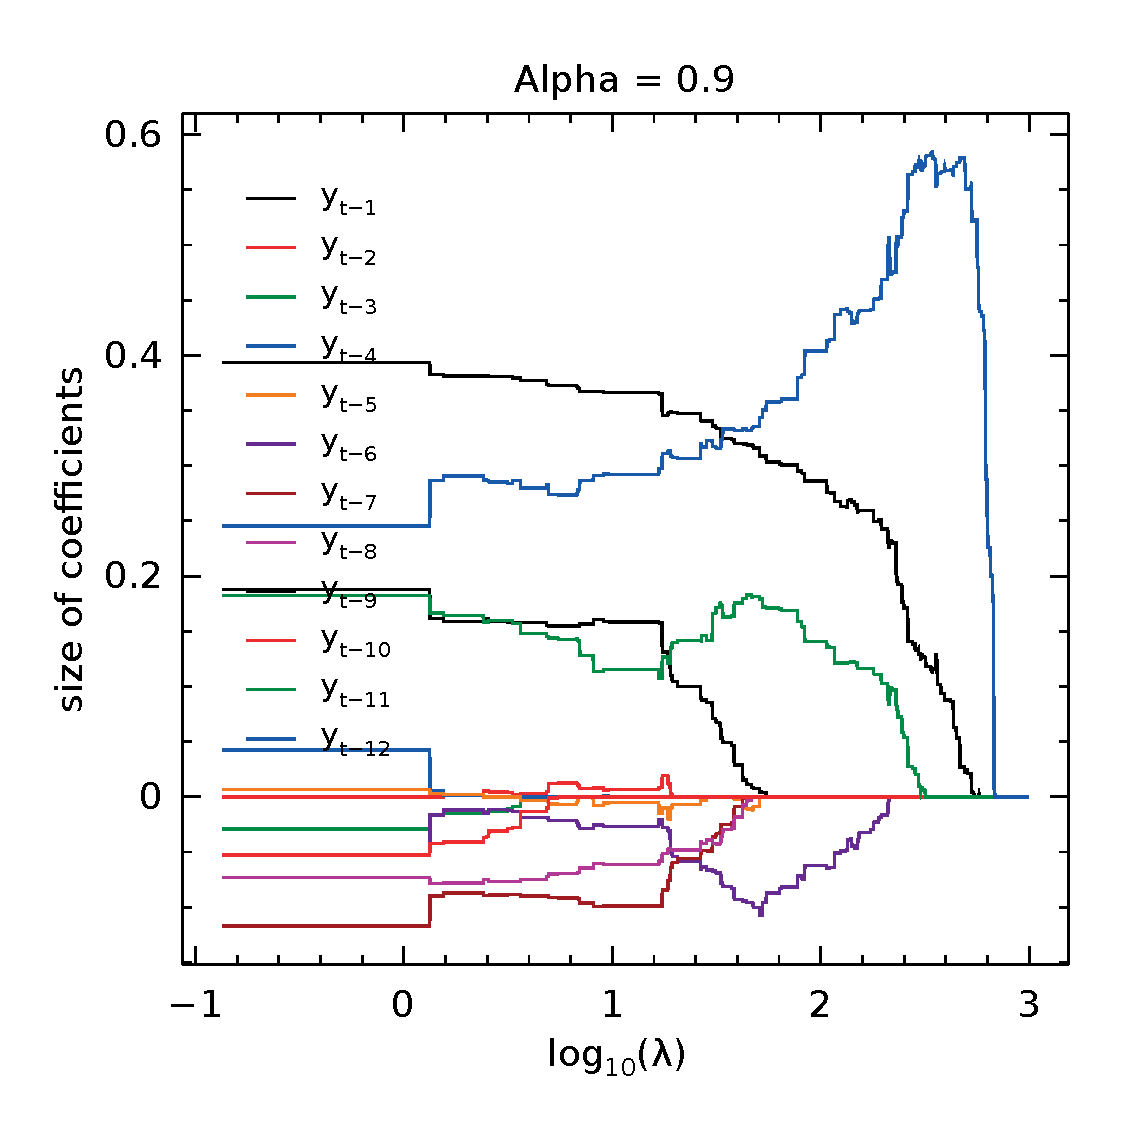
\includegraphics[width=\textwidth]{Figuras/selecao-lasso/par-sellasso-09.pdf}
		\end{minipage}
		\begin{minipage}[b]{\linewidth}
			\centering     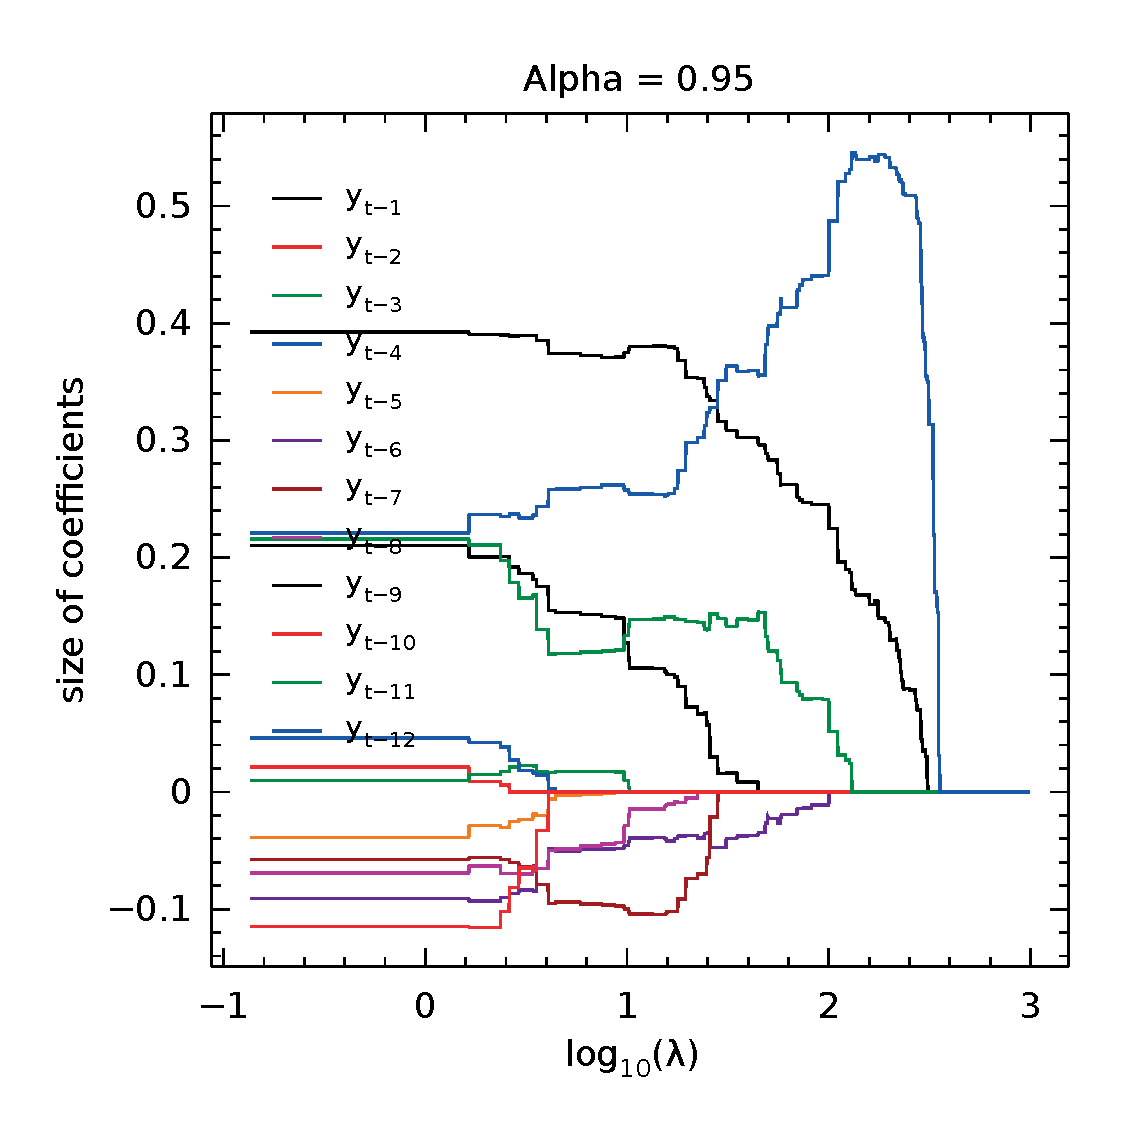
\includegraphics[width=\textwidth]{Figuras/selecao-lasso/par-sellasso-095.pdf}
		\end{minipage}
	\end{minipage}
	\caption{Coefficients path for a few different values of $\alpha$-quantiles. $\lambda$ is presented in a $\log_{10}$ scale, to make visualization easier.}
	\label{fig:lasso-results}
\end{figure}


\subsection{Model selection}

On sections \ref{sec:best-subset-mip} and \ref{sec:best-subset-ell1}, we presented two ways of doing regularization. Nonetheless, regularization can be done with different levels of parsimony. For example, one can select a different number $K$ of variables to be included in the best subset selection via MILP or choose different values of $\lambda$ for the $\ell_1$ penalty. 
%There is a tradeoff between variability and bias, when selecting the number of variables in a model. In order to  

% % % Métrica

Solving a LP problem is much faster than a similar-sized MILP problem. One of our goals is to test how much the LASSO approach gets close to the solution provided when solving the MILP problem. It would be interesting, then, if we could use a faster method that would provide a solution close to the best. To test how far are the solution given by both methods, we propose an experiment that is described as follows. Then, for each number $K$ of total nonzero coefficients, there will be a penalty $\lambda^*_K$ which minimizes the errors from the quantile regression's objective function (given on equation (\ref{eq:post-lasso})): 
%\todo{($K$ ranging from 0 until 12, where 0 means that only the intercept is included)}
\begin{equation}
\lambda^*_K = \argmin_\lambda \left\lbrace \left.  obj_{\lambda}^{*} \quad  \right| \, \| \beta^*_\lambda \|_0 = K \right\rbrace,
\end{equation}
where the quantity $\| \beta^*_\lambda \|_0$ is the $0$-norm, which gives the total of nonzero coefficients, for a given lambda of the LASSO estimations.

We, then, define the sets $L_K^{LASSO}$ and $L_K^{MILP}$, which contains all nonzero indexes, for a given $K$, when using methods LASSO and MILP for regularization, respectively.
Thus, we can compare the best LASSO fit where exactly $K$ variables are selected with the best fit given by the MILP problem, also with $K$ variables selected.

As the MILP solution is the exact solution for the problem, while the LASSO solution is an approximation, we use the former as a \textit{benchmarking} for the quality of the latter solution. To help us view the difference of results between both methods, we define a similarity metric $d$ between the subset of coefficients chosen by each one of them. It is desirable that the LASSO solution be as related with the MILP solution as possible.
The similarity is calculated as the solution of the following optimization problem
\begin{eqnarray}
d(\beta^*_{MILP(K)}, \beta^*_{\lambda^*_K}) = \min_{0\leq\delta_{ij}\leq1} & \sum\limits_{i,j = 1}^K  \delta_{ij} (1-|\rho_{ij}|) \label{eq:metricad0} \\
\text{s.t.} & \sum\limits_{j =1}^K\delta_{ij}=1, &  i=1,\dots,K,\\
& \sum\limits_{i =1}^K\delta_{ij}=1, & j=1,\dots,K,
\end{eqnarray}
where $\rho_{ij}$ is the correlation between the $i$-th and $j$-th independent variables in sets $L_k^{MILP}$ and $L_k^{LASSO}$, respectively. The optimal value for the decision variables of this problem provides us with an assignment between selected covariates from both methods, namely, MILP and LASSO, that minimizes the overall ``index of uncorrelation" between selected covariates. If $\delta^*_{ij} = 1$, the $i$-th selected variable in  $L_k^{MILP}$ is associated with the $j$-th variable  in $L_k^{LASSO}$. For instance, if $d(\beta^*_{MILP(K)}, \beta^*_{\lambda^*_K}) = 0$, it means that there are $K$ perfectly correlated pair of variables, despite not being the same.

% % % Trocar o sigma da função objetivo.




% % % recolocar no texto
As seen before, we have a best solution for each desired $K$. The question that arises now is how to select the ideal number of variables to use.
One way of achieving this is by using an information criteria to guide our decision. 
An information criteria summarizes two aspects. One of them refers to how well the model fits the in-sample observations. The other part penalizes the quantity of covariates used in the model. By penalizing how big our model is, we prevent overfitting from happening. So, in order for a covariate to be included in the model, it must supply enough goodness of fit.
In \cite{machado1993robust}, it is presented a variation of the Schwarz criteria for M-estimators that includes quantile regression. The Schwarz Information Criteria (SIC), adapted to the quantile autoregression case, is presented below:
\begin{align} 
\begin{split}
SIC(m) = n \log(\hat{\sigma}^*)+\frac{1}{2}K\log n,\label{eq:SIC}
\end{split}					
\end{align}
where $K$ is the model's dimension. This procedure leads to a consistent model selection if the model is well specified. 

Figure \ref{fig:comparison-lm-results} shows the results of these experiments for quantiles $\alpha \in \{0.05, 0.1, 0.5, 0.9, 0.95\}$. The results point us that for small values of $K$ the distance between coefficients is bigger and where we observe the biggest differences between the SIC values. In this experiment, the minimum SIC value for the MILP problem is usually found between 4 and 6 variables in the model.

\begin{figure}
	\centering
	\begin{minipage}[t]{0.4\linewidth}
		\centering
		\begin{minipage}[t]{\linewidth}
			\centering     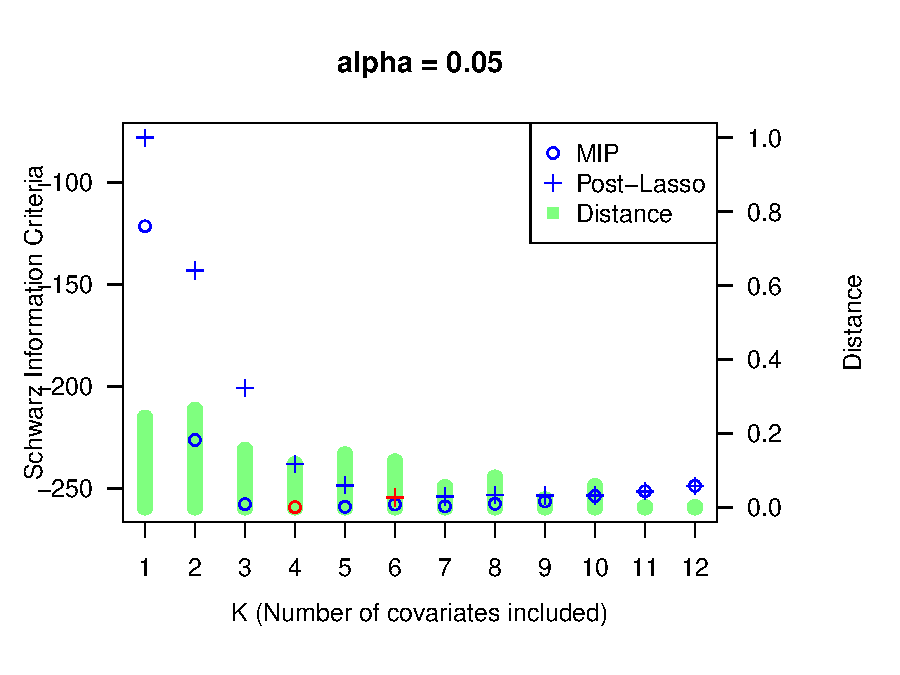
\includegraphics[width=\textwidth]{Figuras/SIC005.pdf}
		\end{minipage}
		\begin{minipage}[b]{\linewidth}
			\centering     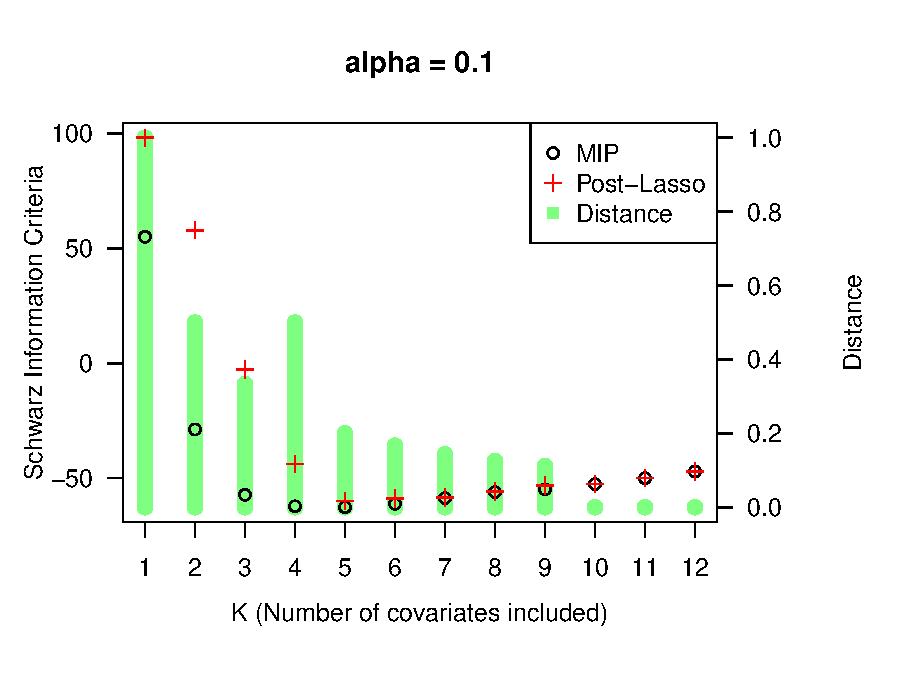
\includegraphics[width=\textwidth]{Figuras/SIC01.pdf}
		\end{minipage}
		\begin{minipage}[b]{\linewidth}
			\centering     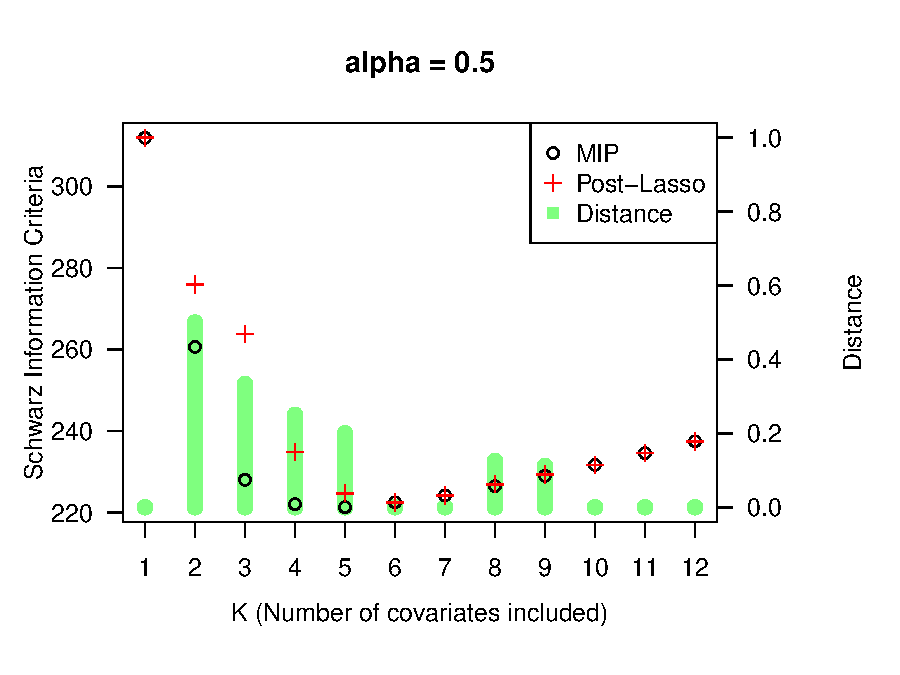
\includegraphics[width=\textwidth]{Figuras/SIC05.pdf}
		\end{minipage}
	\end{minipage}
	\begin{minipage}[t]{0.4\linewidth}
		\centering
		\begin{minipage}[b]{\linewidth}
			\centering     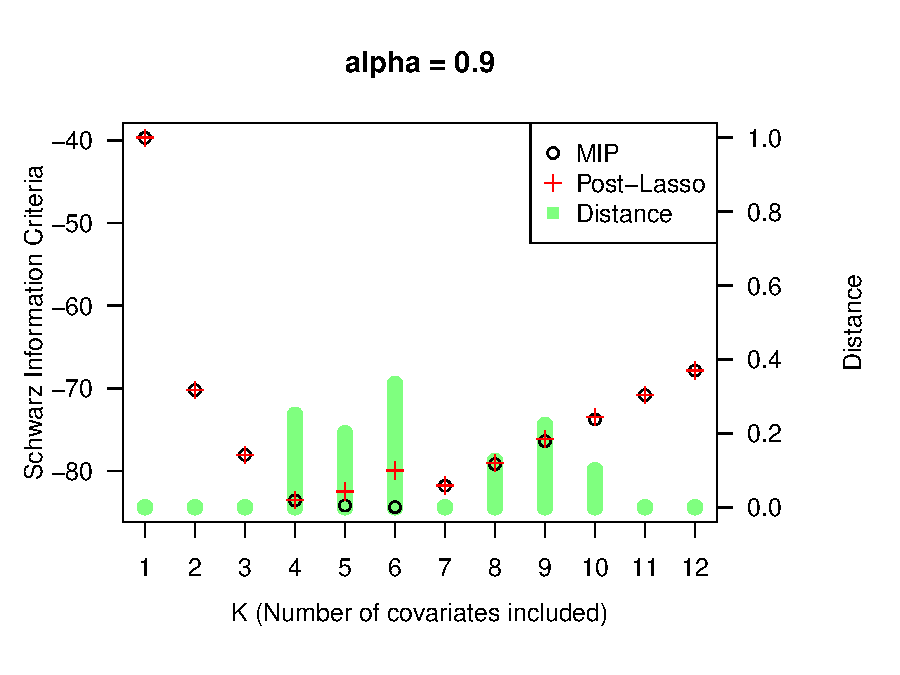
\includegraphics[width=\textwidth]{Figuras/SIC09.pdf}
		\end{minipage}
		\begin{minipage}[b]{\linewidth}
			\centering     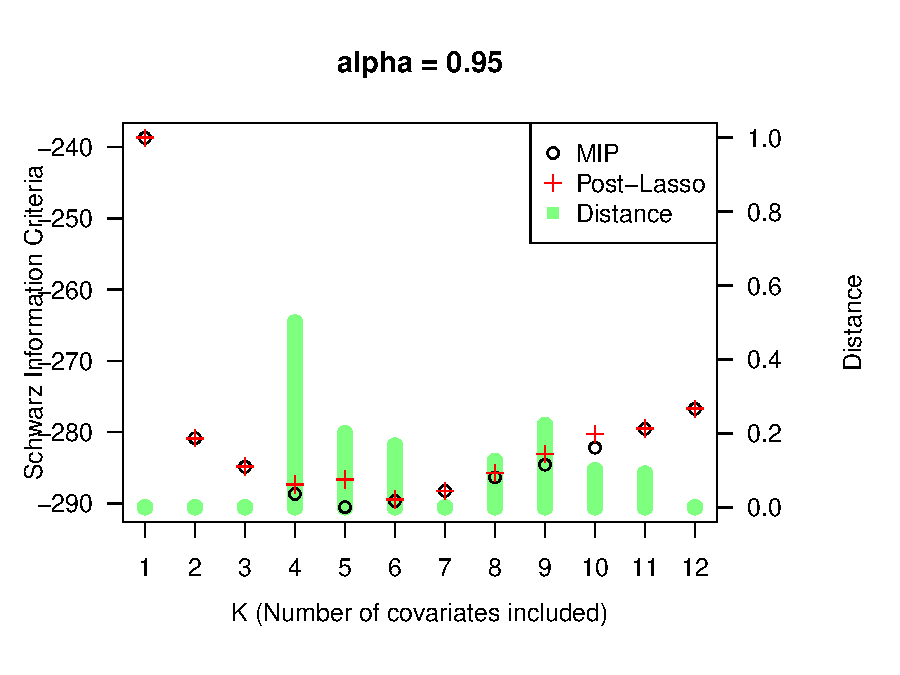
\includegraphics[width=\textwidth]{Figuras/SIC095.pdf}
			\label{fig:npqar-cross}
		\end{minipage}
	\end{minipage}
	\caption{ {Comparison of SIC values when using methods LASSO and MILP as a variable selector}. The Information Criteria is displayed on the y-axis, while the number of variables $K$ included is shown on the x-axis. Both solutions of the MILP and the best LASSO for a given $K$ are  The bars represent the distance $d$ as defined on problem (\ref{eq:metricad0})-(\ref{eq:metricad4}). When $d=0$, it means that the same variables are selected from both methods for a given $K$. Thus, in these cases we have the same SIC for both of them.}
	\label{fig:comparison-lm-results}
\end{figure}


\section{Simulation}
\label{sec:simulation}

In this section, we investigate how to simulate future paths of the time series $y_t$. 
%We use this model to produce $K$ future values for the time serie $y_t$. 
Let $n$ be the total number of observations of $y_t$. We produce $S$ different paths with size $K$ for each. 
We have $n$ observations of $y_t$ and we want to produce . Given a vector of explanatory variables $x_t$, let $q_\alpha(x_t)$ be given by the $\alpha$-quantile estimated as described on section \ref{sec:estimating-distribution}.

The variables chosen to compose $x_t$ can be either exogenous variables, autoregressive components of $y_t$ or both. As the distribution of $\varepsilon_t$ is unknown, we have to use a nonparametric approach in order to estimate its one-step ahead density.

The coefficients $\beta_{0 \alpha}$ and $\beta_{\alpha}$ are the solution of the minimization problem given in the problem defined in (\ref{eq:non-crossing-quantiles1})-(\ref{eq:non-crossing-constraint}), reproduced here for convenience:
\begin{eqnarray}
\min_{q_\alpha,\varepsilon_{t,\alpha}^{+}, \varepsilon_{t,\alpha}^{-}} &  \sum_{\alpha \in A} \sum_{t \in T}\left(\alpha \varepsilon_{t,\alpha}^{+}+(1-\alpha)\varepsilon_{t,\alpha}^{-}\right) &  \\
\mbox{s.t. } & \varepsilon_{t,\alpha}^{+}-\varepsilon_{t,\alpha}^{-}=y_{t} - q_\alpha(x_{t}), & \qquad\forall t \in T_\tau,\forall \alpha \in A,\\
& \varepsilon_{t,\alpha}^+,\varepsilon_{t,\alpha}^- \geq 0, & \qquad\forall t \in T_\tau,\forall \alpha \in A,\\ 
& q_{\alpha}(x_t) \leq q_{\alpha'}(x_t), & \qquad \forall t \in T_\tau, \forall (\alpha, \alpha') \in A \times A,  \alpha < \alpha', 
\end{eqnarray}

To produce $S$ different paths of $\{ \hat{y}_t \}_{t=n+1}^{n+K}$, we use the following procedure:

\noindent\rule{\textwidth}{3pt}

Procedure for simulating $S$ scenarios of $y_t$

\noindent\rule{\textwidth}{1pt}

\begin{enumerate}
	
\item At first, let $\tau = n + 1$.

\item In any given period $\tau$, for every $\alpha \in A$, we use the problem defined on  (\ref{eq:non-crossing-quantiles1})-(\ref{eq:non-crossing-constraint}) to estimate quantiles 
 $q_\alpha(x_{\tau})$.
Note that $x_{\tau}$ is supposed to be known at time $\tau$. In the presence of exogenous variables that are unknown, it is advisable to incorporate its uncertainty by considering different scenarios. In each scenario, though, $x_{\tau}$ must be considered fully known. 
 
\item Let $\hat{Q}_{y_{\tau}|X=x_\tau}(\alpha,x_\tau)$ be the estimated quantile function of ${y}_{\tau}$. 
To estimate $\hat{Q}_{y_{\tau}}$, we first define a discrete quantile function $\tilde{Q}_{y_\tau}$. By mapping every $\alpha \in A$ with its estimated quantile $\hat{q}_{\alpha}$, we define function $\tilde{Q}_{y_{\tau}}$. When we interpolate 

This process is described in more details on section \ref{sec:estimating-distribution}. 

qualquer coisa

\item Once we have a distribution for $y_{n+1}$, we can generate $S$ different simulated values, drawn from the distribution function $\hat{F}_{y_{n+1}} = \hat{Q}^{-1}_{y_{\tau}}$, derived from the quantile function found by doing steps 2 and 3. 
Let $X$ be a random variable with uniform distribution over the interval $[0,1]$. By using results from the Probability Integral Transform, we know that the random variable $F^{-1}_{y_{n+1}}(X)$ has the same distribution as $y_{n+1}$. So, by drawing a sample of size $S$ from $X$ and applying the quantile function $Q_{y_{n+1}}(\alpha)$, we have our sample of size $K$ for $y_{n+1}$.

\item Each one of the $S$ different values for $y_{n+1}$ will be the starting point of a different path. Now, for each $\tau \in [n+2,n+K]$ and $s \in S$, we have to estimate quantiles $q_{\alpha \tau, s}$ and find a quantile function for $\hat{Q}_{y_{\tau,s}}$ just like it was done on steps 2 and 3.
Note that when $\tau > n+2$, every estimate will be scenario dependent, hence there will be $S$ distribution functions estimated for each period $\tau$. From now on, in each path just one new value will be drawn randomly from the one-step ahead distribution function - as opposed to what was carried on step 3, when $S$ values were simulated. As there will be $S$ distribution functions - one for each path, in each period $\tau$ it will be produced exact $S$ values for $y_\tau$, one for its own path. Repeating this step until all values of $\tau$ and $s$ are simulated will give us the full simulations that we are looking for.
\end{enumerate}

\begin{figure}[h]
\centering
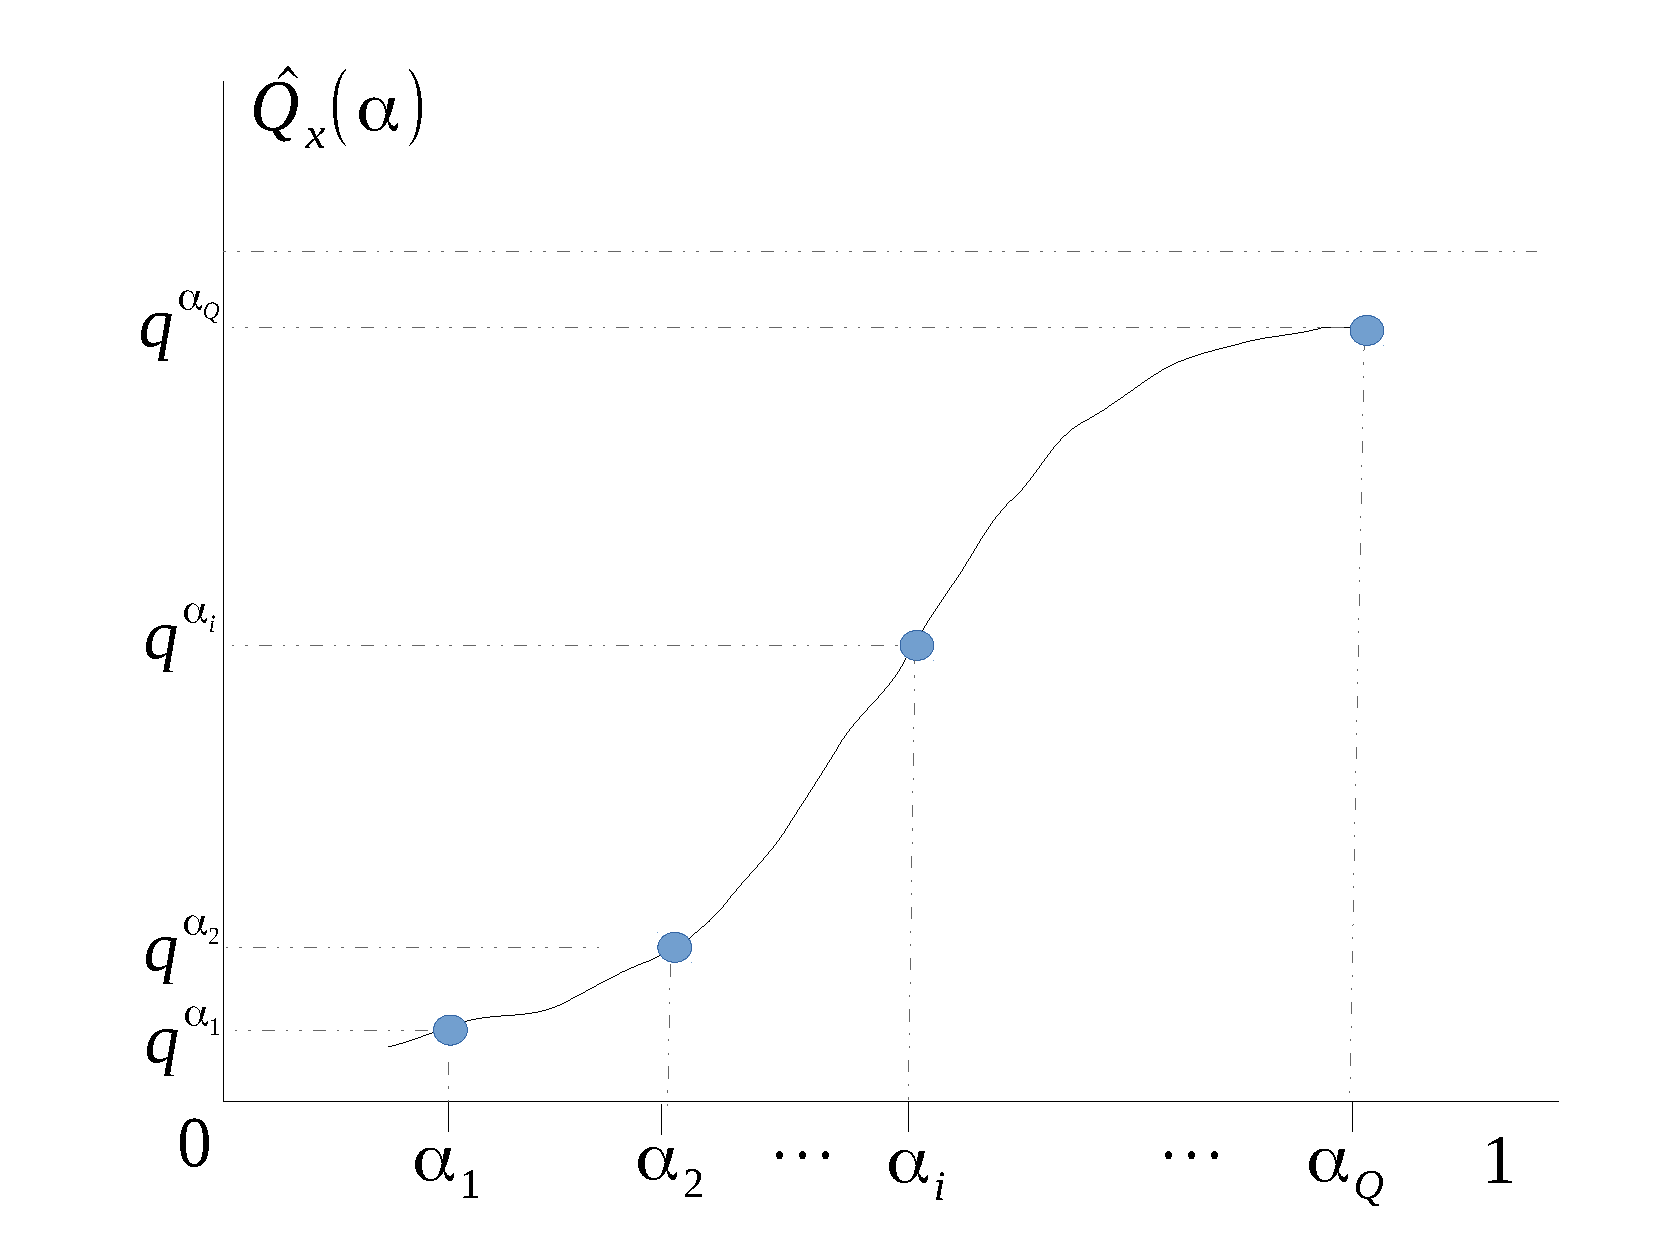
\includegraphics[width=0.7\linewidth]{Figuras/grafico-quantis-fx}
\caption{Fitting a distribution function from quantile estimations}
\label{fig:grafico-quantis-fx}
\end{figure}

%\noindent\rule{\textwidth}{1pt}

\subsection{Simulating for a seasonal time series}

Construir seção
%\section{Conclusion}

\section{Appendices}
\label{appendice}

\subsection{Proof of quantiles as an optimization problem}
\label{sec:quantile-proof}
Let $Z^{\alpha}=\mbox{arg min}_{Q}E[\alpha\max\{0,X-Q\}+(1-\alpha)\max\{0,Q-X\}].$
We can rewrite the function as

\[
\begin{aligned}Y & =\alpha\int_{Q}^{\infty}(X-Q)dF_{x}+(1-\alpha)\int_{-\infty}^{Q}(Q-X)dF_{X}\\
& =\alpha\int_{Q}^{\infty}XdF_{x}-\alpha Q\int_{Q}^{\infty}QdF_{x}+Q\int_{-\infty}^{Q}dF_{x}-\int_{-\infty}^{Q}XdF_{x}-\alpha Q\int_{-\infty}^{Q}dF_{x}+\alpha\int_{-\infty}^{Q}XdF_{x}\\
& =\alpha\int_{Q}^{\infty}XdF_{x}-\alpha Q+QF_{X}(Q)-\int_{-\infty}^{Q}XdF_{x}-\alpha QF_{X}(Q)+\alpha\int_{-\infty}^{Q}XdF_{x}\\
& =\alpha\int_{Q}^{\infty}XdF_{x}-\alpha Q+QF_{X}(Q)-\int_{-\infty}^{Q}XdF_{x}+\alpha\int_{-\infty}^{Q}XdF_{x}
\end{aligned}
\]
By the first order condition for optimality, we need that $\frac{dZ(Q^{*})}{dQ}=0$.
So, we have:

\[
-\alpha Q^{*}f(Q^{*})-\alpha+F_{X}(Q^{*})+Q^{*}f(Q^{*})-Q^{*}f(Q^{*})+\alpha Q^{*}f(Q^{*})=0
\]
\[
F_{X}(Q^{*})=\alpha.
\]
Thus, we have that $Z^\alpha$ is the $\alpha-quantile$ of random variable $X$.

\subsection{MIP coefficients tables}
\label{sec:mipcoefficients}
The following tables inform the size of Coefficients when using the regularization method based on MIP described on session \ref{sec:best-subset-mip}. When using this method, we choose a parameter $K$ which defines the total number of nonzero coefficients (without accounting the intercept $\beta_0$, which is always included). 
In each column we find the estimated values of coefficients for each different choice of $K$. As coefficients are quantile dependent, we provide tables for $\alpha \in (0.05, 0.1, 0.25, 0.5, 0.75, 0.9, 0.95)$.

%\caption{\textbf{$\alpha = 0.05.} 

% latex table generated in R 3.2.3 by xtable 1.7-4 package
% Sat Apr 30 15:33:56 2016
\begin{table}[ht]
\centering
\begin{tabular}{rrrrrrrrrrrrr}
  \hline
 & K=1 & K=2 & K=3 & K=4 & K=5 & K=6 & K=7 & K=8 & K=9 & K=10 & K=11 & K=12 \\ 
  \hline
$\beta_{0}$ & -15.33 & 9.38 & 1.48 & 1.34 & 8.72 & -1.68 & 4.94 & 0.65 & -0.27 & -0.16 & -3.96 & -2.55 \\ 
  $\beta_{1}$ & -0.00 & 0.79 & 0.66 & 0.58 & 0.46 & 0.40 & 0.48 & 0.46 & 0.46 & 0.47 & 0.42 & 0.44 \\ 
  $\beta_{2}$ & -0.00 & -0.00 & -0.00 & -0.00 & -0.00 & 0.33 & -0.00 & -0.00 & -0.00 & -0.00 & 0.14 & 0.09 \\ 
  $\beta_{3}$ & -0.00 & -0.00 & -0.00 & -0.00 & -0.00 & -0.00 & -0.00 & 0.20 & 0.20 & 0.19 & 0.20 & 0.17 \\ 
  $\beta_{4}$ & -0.00 & -0.47 & -0.28 & -0.27 & -0.29 & -0.35 & -0.31 & -0.40 & -0.35 & -0.35 & -0.34 & -0.31 \\ 
  $\beta_{5}$ & -0.00 & -0.00 & -0.00 & -0.00 & -0.00 & -0.00 & -0.00 & -0.00 & -0.00 & -0.05 & -0.07 & -0.09 \\ 
  $\beta_{6}$ & -0.00 & -0.00 & -0.00 & -0.00 & -0.00 & -0.00 & 0.11 & 0.08 & 0.11 & 0.17 & 0.12 & 0.19 \\ 
  $\beta_{7}$ & -0.00 & -0.00 & -0.00 & -0.00 & -0.00 & -0.00 & -0.00 & -0.00 & -0.16 & -0.15 & -0.08 & -0.15 \\ 
  $\beta_{8}$ & -0.00 & -0.00 & -0.00 & -0.00 & -0.15 & -0.00 & -0.31 & -0.26 & -0.17 & -0.17 & -0.16 & -0.18 \\ 
  $\beta_{9}$ & -0.00 & -0.00 & -0.00 & -0.00 & -0.00 & 0.14 & 0.16 & 0.20 & 0.26 & 0.23 & 0.28 & 0.33 \\ 
  $\beta_{10}$ & -0.00 & -0.00 & -0.00 & -0.00 & -0.00 & -0.00 & -0.00 & -0.00 & -0.00 & -0.00 & -0.00 & -0.04 \\ 
  $\beta_{11}$ & -0.00 & -0.00 & 0.26 & 0.17 & 0.21 & 0.08 & 0.16 & 0.19 & 0.17 & 0.18 & 0.17 & 0.20 \\ 
  $\beta_{12}$ & 1.17 & -0.00 & -0.00 & 0.18 & 0.15 & 0.19 & 0.22 & 0.20 & 0.20 & 0.18 & 0.18 & 0.17 \\ 
   \hline
\end{tabular}
\caption{Coefficients for quantile $\alpha = 0.05$}
\end{table}

% latex table generated in R 3.2.3 by xtable 1.8-2 package
% Wed Apr 20 16:50:47 2016
\begin{table}[ht]
\centering
\begin{tabular}{rrrrrrrrrrrrr}
  \hline
 & K=1 & K=2 & K=3 & K=4 & K=5 & K=6 & K=7 & K=8 & K=9 & K=10 & K=11 & K=12 \\ 
  \hline
beta\_0 & -10.68 & 10.07 & 3.56 & 1.24 & 0.76 & 3.01 & 3.33 & 3.02 & 1.05 & 2.26 & 1.55 & 1.57 \\ 
  beta\_1 & -0.00 & 0.81 & 0.63 & 0.61 & 0.55 & 0.49 & 0.49 & 0.50 & 0.48 & 0.44 & 0.44 & 0.44 \\ 
  beta\_2 & -0.00 & -0.00 & -0.00 & -0.00 & -0.00 & -0.00 & 0.04 & -0.00 & -0.00 & 0.04 & 0.07 & 0.07 \\ 
  beta\_3 & -0.00 & -0.00 & -0.00 & -0.00 & 0.15 & 0.20 & 0.16 & 0.15 & 0.13 & 0.11 & 0.12 & 0.12 \\ 
  beta\_4 & -0.00 & -0.43 & -0.33 & -0.28 & -0.37 & -0.33 & -0.34 & -0.30 & -0.24 & -0.24 & -0.26 & -0.25 \\ 
  beta\_5 & -0.00 & -0.00 & -0.00 & -0.00 & -0.00 & -0.08 & -0.07 & -0.12 & -0.14 & -0.15 & -0.17 & -0.17 \\ 
  beta\_6 & -0.00 & -0.00 & -0.00 & -0.00 & -0.00 & -0.00 & -0.00 & 0.11 & 0.10 & 0.10 & 0.14 & 0.14 \\ 
  beta\_7 & -0.00 & -0.00 & -0.00 & -0.00 & -0.00 & -0.00 & -0.00 & -0.07 & -0.11 & -0.13 & -0.11 & -0.11 \\ 
  beta\_8 & -0.00 & -0.00 & -0.00 & -0.00 & -0.00 & -0.00 & -0.00 & -0.00 & -0.00 & -0.00 & -0.04 & -0.04 \\ 
  beta\_9 & -0.00 & -0.00 & -0.00 & -0.00 & -0.00 & -0.00 & -0.00 & -0.00 & 0.09 & 0.10 & 0.13 & 0.13 \\ 
  beta\_10 & -0.00 & -0.00 & -0.00 & -0.00 & -0.00 & -0.00 & -0.00 & -0.00 & -0.00 & -0.00 & -0.00 & 0.00 \\ 
  beta\_11 & -0.00 & -0.00 & -0.00 & 0.14 & 0.17 & 0.17 & 0.16 & 0.15 & 0.11 & 0.09 & 0.08 & 0.08 \\ 
  beta\_12 & 1.09 & -0.00 & 0.35 & 0.27 & 0.25 & 0.22 & 0.22 & 0.26 & 0.33 & 0.34 & 0.33 & 0.33 \\ 
   \hline
\end{tabular}
\end{table}

% latex table generated in R 3.2.3 by xtable 1.7-4 package
% Mon Apr 18 18:43:05 2016
\begin{table}[ht]
\centering
\begin{tabular}{rrrrrrrrrrrrr}
  \hline
 & K=1 & K=2 & K=3 & K=4 & K=5 & K=6 & K=7 & K=8 & K=9 & K=10 & K=11 & K=12 \\ 
  \hline
beta\_0 & 2.72 & -3.38 & 8.64 & 4.88 & 0.62 & 2.98 & 2.70 & 2.62 & 2.27 & 1.87 & 2.43 & 2.53 \\ 
  beta\_1 & -0.00 & 0.59 & 0.52 & 0.51 & 0.57 & 0.54 & 0.56 & 0.56 & 0.58 & 0.58 & 0.57 & 0.57 \\ 
  beta\_2 & -0.00 & -0.00 & -0.00 & -0.00 & -0.00 & -0.00 & -0.00 & -0.00 & -0.03 & -0.06 & -0.05 & -0.05 \\ 
  beta\_3 & -0.00 & -0.00 & -0.00 & -0.00 & -0.00 & -0.00 & -0.00 & -0.00 & -0.00 & 0.04 & 0.03 & 0.04 \\ 
  beta\_4 & -0.00 & -0.00 & -0.25 & -0.18 & -0.14 & -0.11 & -0.11 & -0.12 & -0.11 & -0.11 & -0.11 & -0.12 \\ 
  beta\_5 & -0.00 & -0.00 & -0.00 & -0.00 & -0.00 & -0.00 & -0.00 & -0.00 & -0.00 & -0.00 & -0.00 & 0.01 \\ 
  beta\_6 & -0.00 & -0.00 & -0.00 & -0.00 & -0.00 & -0.06 & -0.09 & -0.08 & -0.08 & -0.08 & -0.09 & -0.09 \\ 
  beta\_7 & -0.00 & -0.00 & -0.00 & -0.00 & -0.00 & -0.00 & -0.00 & -0.00 & -0.00 & -0.00 & -0.02 & -0.02 \\ 
  beta\_8 & -0.00 & -0.00 & -0.00 & -0.00 & -0.00 & -0.00 & 0.06 & 0.06 & 0.05 & 0.06 & 0.08 & 0.07 \\ 
  beta\_9 & -0.00 & -0.00 & -0.00 & -0.00 & 0.08 & 0.09 & 0.06 & 0.09 & 0.07 & 0.07 & 0.08 & 0.08 \\ 
  beta\_10 & -0.00 & -0.00 & -0.00 & -0.00 & -0.00 & -0.00 & -0.00 & -0.05 & -0.04 & -0.05 & -0.05 & -0.05 \\ 
  beta\_11 & -0.00 & 0.54 & -0.00 & 0.15 & 0.14 & 0.11 & 0.10 & 0.11 & 0.14 & 0.14 & 0.15 & 0.14 \\ 
  beta\_12 & 0.92 & -0.00 & 0.42 & 0.34 & 0.32 & 0.33 & 0.32 & 0.34 & 0.33 & 0.34 & 0.32 & 0.33 \\ 
   \hline
\end{tabular}
\end{table}

% latex table generated in R 3.2.3 by xtable 1.7-4 package
% Mon Apr 18 18:43:05 2016
\begin{table}[ht]
\centering
\begin{tabular}{rrrrrrrrrrrrr}
  \hline
 & K=1 & K=2 & K=3 & K=4 & K=5 & K=6 & K=7 & K=8 & K=9 & K=10 & K=11 & K=12 \\ 
  \hline
beta\_0 & 12.14 & 10.06 & 6.60 & 11.05 & 13.22 & 12.04 & 13.34 & 13.28 & 12.58 & 13.69 & 13.47 & 13.71 \\ 
  beta\_1 & -0.00 & 0.24 & 0.39 & 0.39 & 0.40 & 0.38 & 0.38 & 0.38 & 0.38 & 0.40 & 0.40 & 0.40 \\ 
  beta\_2 & -0.00 & -0.00 & -0.00 & -0.00 & -0.00 & -0.00 & -0.00 & -0.00 & -0.00 & -0.00 & -0.00 & -0.02 \\ 
  beta\_3 & -0.00 & -0.00 & -0.00 & -0.00 & -0.00 & -0.00 & -0.00 & -0.00 & -0.01 & -0.04 & -0.03 & -0.02 \\ 
  beta\_4 & -0.00 & -0.00 & -0.00 & -0.00 & -0.00 & -0.00 & -0.00 & 0.03 & -0.00 & 0.05 & 0.05 & 0.04 \\ 
  beta\_5 & -0.00 & -0.00 & -0.00 & -0.00 & -0.00 & -0.00 & -0.00 & -0.00 & -0.00 & -0.00 & 0.00 & 0.01 \\ 
  beta\_6 & -0.00 & -0.00 & -0.00 & -0.14 & -0.00 & -0.00 & -0.03 & -0.05 & -0.01 & -0.07 & -0.07 & -0.07 \\ 
  beta\_7 & -0.00 & -0.00 & -0.00 & -0.00 & -0.19 & -0.10 & -0.10 & -0.11 & -0.09 & -0.11 & -0.11 & -0.10 \\ 
  beta\_8 & -0.00 & -0.00 & -0.00 & -0.00 & -0.00 & -0.08 & -0.07 & -0.08 & -0.08 & -0.07 & -0.07 & -0.08 \\ 
  beta\_9 & -0.00 & -0.00 & -0.00 & 0.14 & 0.16 & 0.15 & 0.16 & 0.18 & 0.16 & 0.19 & 0.19 & 0.19 \\ 
  beta\_10 & -0.00 & -0.00 & -0.00 & -0.00 & -0.00 & -0.00 & -0.00 & -0.00 & -0.04 & -0.06 & -0.06 & -0.06 \\ 
  beta\_11 & -0.00 & -0.00 & 0.20 & -0.00 & 0.11 & 0.15 & 0.12 & 0.16 & 0.16 & 0.18 & 0.18 & 0.19 \\ 
  beta\_12 & 0.80 & 0.63 & 0.39 & 0.42 & 0.26 & 0.29 & 0.28 & 0.23 & 0.29 & 0.24 & 0.24 & 0.25 \\ 
   \hline
\end{tabular}
\end{table}

% latex table generated in R 3.2.3 by xtable 1.7-4 package
% Sat Apr 30 15:33:56 2016
\begin{table}[ht]
\centering
\begin{tabular}{rrrrrrrrrrrrr}
  \hline
 & K=1 & K=2 & K=3 & K=4 & K=5 & K=6 & K=7 & K=8 & K=9 & K=10 & K=11 & K=12 \\ 
  \hline
$\beta_{0}$ & 16.73 & 11.74 & 11.51 & 13.77 & 13.45 & 13.48 & 14.36 & 14.84 & 12.36 & 14.04 & 13.09 & 14.00 \\ 
  $\beta_{1}$ & -0.00 & 0.26 & 0.32 & 0.35 & 0.38 & 0.38 & 0.40 & 0.43 & 0.40 & 0.40 & 0.39 & 0.39 \\ 
  $\beta_{2}$ & -0.00 & -0.00 & -0.00 & -0.00 & -0.00 & -0.00 & -0.00 & -0.00 & -0.00 & -0.00 & 0.02 & 0.02 \\ 
  $\beta_{3}$ & -0.00 & -0.00 & -0.00 & -0.00 & -0.00 & -0.00 & -0.00 & -0.00 & -0.00 & -0.00 & -0.00 & 0.01 \\ 
  $\beta_{4}$ & -0.00 & -0.00 & -0.00 & -0.00 & -0.00 & -0.00 & -0.00 & -0.00 & 0.04 & 0.06 & 0.06 & 0.05 \\ 
  $\beta_{5}$ & -0.00 & -0.00 & -0.00 & -0.00 & -0.00 & -0.00 & -0.00 & -0.00 & -0.00 & -0.04 & -0.03 & -0.04 \\ 
  $\beta_{6}$ & -0.00 & -0.00 & -0.00 & -0.00 & -0.00 & -0.00 & -0.05 & -0.10 & -0.07 & -0.09 & -0.08 & -0.09 \\ 
  $\beta_{7}$ & -0.00 & -0.00 & -0.00 & -0.15 & -0.14 & -0.12 & -0.09 & -0.05 & -0.06 & -0.06 & -0.06 & -0.06 \\ 
  $\beta_{8}$ & -0.00 & -0.00 & -0.00 & -0.00 & -0.00 & -0.04 & -0.05 & -0.07 & -0.05 & -0.08 & -0.07 & -0.07 \\ 
  $\beta_{9}$ & -0.00 & -0.00 & -0.00 & 0.16 & 0.11 & 0.14 & 0.16 & 0.19 & 0.19 & 0.22 & 0.22 & 0.21 \\ 
  $\beta_{10}$ & -0.00 & -0.00 & -0.00 & -0.00 & -0.00 & -0.00 & -0.00 & -0.15 & -0.14 & -0.11 & -0.12 & -0.11 \\ 
  $\beta_{11}$ & -0.00 & -0.00 & 0.17 & -0.00 & 0.14 & 0.13 & 0.12 & 0.25 & 0.23 & 0.18 & 0.21 & 0.22 \\ 
  $\beta_{12}$ & 0.71 & 0.59 & 0.37 & 0.41 & 0.28 & 0.28 & 0.25 & 0.21 & 0.27 & 0.25 & 0.24 & 0.22 \\ 
   \hline
\end{tabular}
\end{table}

% latex table generated in R 3.3.2 by xtable 1.8-2 package
% Thu Feb  9 18:57:39 2017
\begin{table}[ht]
\centering
\begin{tabular}{rrrrrrrrrrrrr}
  \hline
 & Jan & Feb & Mar & Apr & May & Jun & Jul & Aug & Sep & Oct & Nov & Dec \\ 
  \hline
1981 & 23.36 & 28.34 & 12.44 & 18.35 & 17.10 & 22.49 & 23.57 & 40.10 & 48.40 & 42.13 & 43.70 & 37.23 \\ 
  1982 & 20.54 & 17.48 & 7.42 & 10.87 & 16.57 & 20.79 & 27.95 & 42.55 & 49.12 & 42.48 & 44.78 & 40.20 \\ 
  1983 & 27.94 & 24.50 & 22.60 & 22.24 & 29.62 & 27.05 & 33.92 & 45.06 & 50.64 & 49.32 & 43.83 & 36.14 \\ 
  1984 & 20.37 & 15.35 & 3.94 & 3.57 & 7.85 & 14.65 & 20.56 & 41.01 & 44.58 & 44.31 & 42.94 & 31.65 \\ 
  1985 & 10.38 & 4.71 & 5.15 & 2.84 & 7.27 & 10.36 & 14.53 & 39.33 & 45.18 & 41.21 & 42.15 & 23.02 \\ 
  1986 & 18.86 & 8.25 & 3.00 & 5.23 & 17.29 & 17.85 & 23.08 & 41.36 & 48.30 & 42.83 & 44.36 & 36.41 \\ 
  1987 & 26.09 & 24.71 & 6.90 & 21.02 & 20.73 & 19.53 & 28.42 & 42.94 & 48.06 & 44.26 & 43.11 & 39.67 \\ 
  1988 & 15.75 & 11.66 & 4.51 & 4.36 & 8.29 & 11.50 & 19.10 & 38.40 & 46.47 & 44.80 & 41.79 & 22.40 \\ 
  1989 & 19.92 & 14.52 & 5.08 & 2.75 & 5.62 & 11.42 & 17.17 & 38.94 & 43.92 & 43.70 & 40.69 & 26.34 \\ 
  1990 & 29.74 & 11.70 & 15.69 & 14.02 & 14.85 & 22.28 & 24.02 & 44.55 & 48.18 & 44.66 & 41.51 & 32.41 \\ 
  1991 & 17.09 & 13.46 & 7.68 & 6.63 & 8.51 & 16.17 & 26.46 & 43.36 & 49.00 & 45.86 & 40.14 & 36.57 \\ 
  1992 & 21.41 & 19.78 & 14.25 & 21.45 & 24.24 & 24.64 & 30.34 & 45.43 & 51.33 & 47.66 & 44.50 & 37.97 \\ 
  1993 & 27.86 & 20.13 & 14.36 & 16.63 & 20.94 & 26.43 & 30.60 & 44.07 & 44.73 & 43.78 & 41.40 & 34.18 \\ 
  1994 & 12.45 & 11.06 & 4.70 & 5.85 & 10.49 & 11.04 & 23.03 & 38.50 & 48.92 & 47.30 & 44.97 & 36.55 \\ 
  1995 & 20.31 & 5.80 & 9.47 & 5.36 & 5.62 & 14.15 & 23.54 & 42.48 & 50.49 & 42.74 & 41.15 & 29.90 \\ 
  1996 & 19.89 & 11.85 & 3.43 & 5.08 & 8.26 & 16.29 & 24.89 & 40.52 & 48.44 & 44.92 & 40.15 & 36.37 \\ 
  1997 & 23.89 & 27.80 & 14.30 & 11.95 & 17.55 & 22.22 & 31.82 & 44.07 & 43.14 & 40.00 & 37.94 & 28.36 \\ 
  1998 & 15.04 & 21.70 & 10.61 & 17.28 & 21.57 & 22.31 & 27.26 & 42.45 & 49.04 & 46.76 & 37.22 & 35.74 \\ 
  1999 & 22.18 & 15.39 & 8.18 & 13.66 & 8.67 & 16.49 & 22.30 & 40.43 & 47.75 & 39.85 & 36.95 & 35.54 \\ 
  2000 & 16.75 & 7.95 & 11.33 & 10.47 & 16.73 & 15.07 & 18.90 & 38.91 & 44.26 & 46.34 & 41.98 & 31.62 \\ 
  2001 & 24.03 & 11.82 & 11.09 & 9.23 & 16.30 & 14.53 & 25.73 & 41.57 & 45.79 & 40.99 & 41.52 & 42.76 \\ 
  2002 & 16.81 & 22.08 & 13.40 & 11.07 & 15.71 & 17.52 & 26.55 & 41.64 & 45.80 & 45.94 & 40.64 & 30.58 \\ 
  2003 & 17.42 & 14.05 & 10.03 & 11.26 & 15.39 & 17.01 & 28.29 & 39.98 & 47.02 & 47.07 & 40.47 & 34.85 \\ 
  2004 & 15.04 & 13.34 & 17.84 & 16.97 & 20.10 & 19.48 & 25.03 & 40.11 & 48.25 & 47.21 & 44.13 & 35.79 \\ 
  2005 & 24.89 & 20.47 & 13.01 & 20.88 & 19.98 & 21.48 & 27.81 & 42.74 & 46.09 & 46.93 & 44.98 & 36.08 \\ 
  2006 & 32.48 & 15.44 & 12.93 & 6.59 & 12.19 & 19.08 & 27.79 & 40.72 & 46.01 & 44.38 & 42.85 & 33.99 \\ 
  2007 & 28.93 & 11.13 & 16.10 & 11.91 & 17.68 & 21.57 & 30.56 & 42.95 & 47.80 & 47.61 & 42.97 & 35.98 \\ 
  2008 & 20.42 & 15.46 & 3.51 & 9.37 & 8.71 & 13.02 & 23.61 & 36.93 & 45.82 & 46.49 & 43.91 & 35.19 \\ 
  2009 & 21.48 & 15.16 & 6.74 & 3.80 & 4.48 & 12.88 & 24.53 & 38.40 & 47.70 & 40.87 & 46.73 & 38.03 \\ 
  2010 & 24.75 & 30.70 & 16.99 & 16.95 & 15.72 & 16.86 & 27.43 & 43.18 & 48.71 & 35.79 & 41.30 & 30.15 \\ 
  2011 & 16.33 & 14.79 & 9.30 & 7.70 & 13.35 & 18.60 & 23.53 & 39.62 & 46.97 & 40.99 & 44.75 & 42.79 \\ 
   \hline
\end{tabular}
\end{table}



%\subsection{Simulation study tables}
%\label{sec:simulation-tables}
%
%On section \ref{sec:simulation-ar1} we explain a simulation study to try evaluating differences between estimating a quantile with a quantile regression model or using the conditional mean when knowing the true generating model. From this experiment, we present below table of results for three different aspects, for five different quantiles. Tables from \ref{tab:sim-rmse-005} to \ref{tab:sim-rmse-095}  shows the difference between the root mean square errors between both methods of predicting the one-step ahead quantile for a few different values of $\alpha$. Tables \ref{tab:sim-auto-005}-\ref{tab:sim-auto-095} are the ones that shows the nominal difference between the autoregressive coefficients $\hat{\phi}$ and $\hat{\beta}$. The nominal difference between the intercept terms $\hat{\phi}_0 + z_\alpha  \hat{\sigma}^2_\varepsilon)$ and $\hat{\beta}_0)$ is 
%
%% latex table generated in R 3.2.3 by xtable 1.8-2 package
% Tue May 24 17:06:45 2016
\begin{table}[ht]
\centering
\begin{tabular}{rrrrrr}
  \hline
$\phi \backslash RSN$ & 0.01 & 0.05 & 0.1 & 0.5 & 1 \\ 
  \hline
0.25 & 0.99454499 & 0.99987753 & 0.99726238 & 0.99996553 & 0.99997820 \\ 
  0.50 & 0.99928262 & 1.00002733 & 0.99902661 & 1.00017501 & 1.00072601 \\ 
  0.70 & 0.97952103 & 0.99154652 & 1.00049301 & 0.99991315 & 1.00014586 \\ 
  0.90 & 0.89928729 & 0.99117750 & 0.99730087 & 1.00106737 & 0.99970135 \\ 
   \hline
\end{tabular}
\caption{RMSE ratio ($RMSE^{QR} / RMSE^{AR} $) for estimating quantile
$\alpha = $ 0.05. $\phi$ stands for the autoregressive coefficient 
and RSN is the signal to noise ratio. Details for these experiments can 
be found on section \ref{sec:simulation-ar1}} 
\label{tab:sim-rmse-005}
\end{table}

%% latex table generated in R 3.2.3 by xtable 1.8-2 package
% Tue May 24 17:06:45 2016
\begin{table}[ht]
\centering
\begin{tabular}{rrrrrr}
  \hline
$\phi \backslash RSN$ & 0.01 & 0.05 & 0.1 & 0.5 & 1 \\ 
  \hline
0.25 & 0.99404378 & 1.00071379 & 0.99865043 & 1.00009650 & 1.00031150 \\ 
  0.50 & 0.99302385 & 1.00012893 & 1.00008177 & 1.00020172 & 0.99997679 \\ 
  0.70 & 0.96163465 & 0.99948879 & 1.00007350 & 1.00076714 & 1.00002219 \\ 
  0.90 & 0.82867689 & 0.99989835 & 1.00007245 & 0.99997754 & 1.00016876 \\ 
   \hline
\end{tabular}
\caption{RMSE ratio ($RMSE^{QR} / RMSE^{AR} $) for estimating quantile
$\alpha = $ 0.1. $\phi$ stands for the autoregressive coefficient 
and RSN is the signal to noise ratio. Details for these experiments can 
be found on section \ref{sec:simulation-ar1}} 
\label{tab:sim-rmse-01}
\end{table}

%% latex table generated in R 3.2.3 by xtable 1.8-2 package
% Tue May 24 17:06:46 2016
\begin{table}[ht]
\centering
\begin{tabular}{rrrrrr}
  \hline
$\phi \backslash RSN$ & 0.01 & 0.05 & 0.1 & 0.5 & 1 \\ 
  \hline
0.25 & 0.98066380 & 0.99981708 & 0.99972368 & 1.00003875 & 1.00027661 \\ 
  0.50 & 0.99671712 & 0.99884992 & 0.99718531 & 0.99996169 & 0.99939155 \\ 
  0.70 & 0.96160330 & 0.99971110 & 1.00006113 & 1.00001116 & 1.00024519 \\ 
  0.90 & 0.93616426 & 0.99985323 & 0.99934405 & 0.99991411 & 0.99994730 \\ 
   \hline
\end{tabular}
\caption{RMSE ratio ($RMSE^{QR} / RMSE^{AR} $) for estimating quantile
$\alpha = $ 0.5. $\phi$ stands for the autoregressive coefficient 
and RSN is the signal to noise ratio. Details for these experiments can 
be found on section \ref{sec:simulation-ar1}} 
\label{tab:sim-rmse-05}
\end{table}

%% latex table generated in R 3.2.3 by xtable 1.8-2 package
% Tue May 24 17:06:46 2016
\begin{table}[ht]
\centering
\begin{tabular}{rrrrrr}
  \hline
$\phi \backslash RSN$ & 0.01 & 0.05 & 0.1 & 0.5 & 1 \\ 
  \hline
0.25 & 0.99662610 & 0.99945043 & 0.99538478 & 0.99966478 & 1.00025526 \\ 
  0.50 & 1.00028533 & 0.99613341 & 0.99981279 & 0.99996292 & 1.00108295 \\ 
  0.70 & 0.91878126 & 0.99889801 & 0.99885007 & 1.00023457 & 1.00067966 \\ 
  0.90 & 0.80536841 & 0.99826964 & 0.99806239 & 1.00003275 & 0.99993464 \\ 
   \hline
\end{tabular}
\caption{RMSE ratio ($RMSE^{QR} / RMSE^{AR} $) for estimating quantile
$\alpha = $ 0.9. $\phi$ stands for the autoregressive coefficient 
and RSN is the signal to noise ratio. Details for these experiments can 
be found on section \ref{sec:simulation-ar1}} 
\label{tab:sim-rmse-09}
\end{table}

%% latex table generated in R 3.2.3 by xtable 1.8-2 package
% Tue May 24 17:06:46 2016
\begin{table}[ht]
\centering
\begin{tabular}{rrrrrr}
  \hline
$\phi \backslash RSN$ & 0.01 & 0.05 & 0.1 & 0.5 & 1 \\ 
  \hline
0.25 & 1.00009586 & 0.99962843 & 1.00162321 & 1.00002799 & 1.00023607 \\ 
  0.50 & 0.99977885 & 0.99742853 & 0.99415437 & 1.00058173 & 0.99971703 \\ 
  0.70 & 0.93295124 & 0.99948015 & 0.99936096 & 1.00048504 & 0.99969376 \\ 
  0.90 & 0.97068193 & 1.00001858 & 1.00007662 & 1.00020540 & 0.99928392 \\ 
   \hline
\end{tabular}
\caption{RMSE ratio ($RMSE^{QR} / RMSE^{AR} $) for estimating quantile
$\alpha = $ 0.95. $\phi$ stands for the autoregressive coefficient 
and RSN is the signal to noise ratio. Details for these experiments can 
be found on section \ref{sec:simulation-ar1}} 
\label{tab:sim-rmse-095}
\end{table}

%
%% latex table generated in R 3.2.3 by xtable 1.8-2 package
% Tue May 24 17:06:45 2016
\begin{table}[ht]
\centering
\begin{tabular}{rrrrrr}
  \hline
$\phi \backslash RSN$ & 0.01 & 0.05 & 0.1 & 0.5 & 1 \\ 
  \hline
0.25 & -0.02501316 & 0.01504215 & -0.00565925 & -0.01735387 & -0.00060544 \\ 
  0.50 & -0.01319163 & 0.00222293 & 0.00477565 & 0.01005289 & -0.01981673 \\ 
  0.70 & 0.02775786 & -0.01203545 & 0.01320180 & -0.00721887 & -0.00665778 \\ 
  0.90 & 0.01743705 & 0.00303553 & 0.01319473 & -0.01785909 & 0.00046374 \\ 
   \hline
\end{tabular}
\caption{Diffeference between the autoregressive coefficients ($\hat{\phi} - \hat{\beta}$) for estimating quantile
$\alpha = $ 0.05. $\phi$ stands for the autoregressive coefficient 
and RSN is the signal to noise ratio. Details for these experiments can 
be found on section \ref{sec:simulation-ar1}} 
\label{tab:sim-auto-005}
\end{table}

%% latex table generated in R 3.2.3 by xtable 1.8-2 package
% Tue May 24 17:06:46 2016
\begin{table}[ht]
\centering
\begin{tabular}{rrrrrr}
  \hline
$\phi \backslash RSN$ & 0.01 & 0.05 & 0.1 & 0.5 & 1 \\ 
  \hline
0.25 & -0.00866846 & 0.02731984 & 0.01494079 & -0.01572119 & 0.01000855 \\ 
  0.50 & 0.02547593 & 0.00642516 & 0.00247766 & -0.00871352 & 0.00277974 \\ 
  0.70 & 0.00503748 & 0.00751987 & -0.00107390 & 0.00327506 & -0.00044987 \\ 
  0.90 & 0.00709175 & 0.00692367 & -0.00624776 & 0.00298916 & -0.00493012 \\ 
   \hline
\end{tabular}
\caption{Diffeference between the autoregressive coefficients ($\hat{\phi} - \hat{\beta}$) for estimating quantile
$\alpha = $ 0.1. $\phi$ stands for the autoregressive coefficient 
and RSN is the signal to noise ratio. Details for these experiments can 
be found on section \ref{sec:simulation-ar1}} 
\label{tab:sim-auto-01}
\end{table}

%% latex table generated in R 3.2.3 by xtable 1.8-2 package
% Tue May 24 17:06:46 2016
\begin{table}[ht]
\centering
\begin{tabular}{rrrrrr}
  \hline
$\phi \backslash RSN$ & 0.01 & 0.05 & 0.1 & 0.5 & 1 \\ 
  \hline
0.25 & 0.00504450 & -0.00552938 & 0.00198665 & 0.00331038 & 0.00493278 \\ 
  0.50 & 0.00816919 & -0.00518034 & -0.00514326 & 0.00056696 & 0.00347201 \\ 
  0.70 & 0.00817503 & 0.00319246 & -0.00703127 & -0.00478434 & 0.00539972 \\ 
  0.90 & 0.01257091 & 0.00502689 & -0.00469782 & -0.00543626 & 0.00172323 \\ 
   \hline
\end{tabular}
\caption{Diffeference between the autoregressive coefficients ($\hat{\phi} - \hat{\beta}$) for estimating quantile
$\alpha = $ 0.5. $\phi$ stands for the autoregressive coefficient 
and RSN is the signal to noise ratio. Details for these experiments can 
be found on section \ref{sec:simulation-ar1}} 
\label{tab:sim-auto-05}
\end{table}

%% latex table generated in R 3.2.3 by xtable 1.8-2 package
% Tue May 24 17:06:46 2016
\begin{table}[ht]
\centering
\begin{tabular}{rrrrrr}
  \hline
$\phi \backslash RSN$ & 0.01 & 0.05 & 0.1 & 0.5 & 1 \\ 
  \hline
0.25 & 0.00063949 & -0.00587333 & -0.00343132 & 0.00057888 & -0.01576153 \\ 
  0.50 & -0.01953741 & -0.00099696 & -0.01220643 & -0.00459181 & -0.02725897 \\ 
  0.70 & 0.00879188 & -0.00578564 & -0.01365016 & -0.01735324 & -0.01595786 \\ 
  0.90 & -0.00432531 & -0.00674863 & 0.00059043 & 0.00040195 & 0.00452383 \\ 
   \hline
\end{tabular}
\caption{Diffeference between the autoregressive coefficients ($\hat{\phi} - \hat{\beta}$) for estimating quantile
$\alpha = $ 0.9. $\phi$ stands for the autoregressive coefficient 
and RSN is the signal to noise ratio. Details for these experiments can 
be found on section \ref{sec:simulation-ar1}} 
\label{tab:sim-auto-09}
\end{table}

%% latex table generated in R 3.2.3 by xtable 1.8-2 package
% Tue May 24 17:06:46 2016
\begin{table}[ht]
\centering
\begin{tabular}{rrrrrr}
  \hline
$\phi \backslash RSN$ & 0.01 & 0.05 & 0.1 & 0.5 & 1 \\ 
  \hline
0.25 & -0.00217703 & 0.01773060 & -0.01892853 & 0.01070602 & -0.01105531 \\ 
  0.50 & -0.01530692 & -0.01035399 & -0.02514421 & 0.01278911 & -0.00835432 \\ 
  0.70 & 0.04323376 & -0.00354721 & 0.03589676 & -0.00176410 & -0.00545403 \\ 
  0.90 & 0.04279246 & 0.00727074 & -0.00552405 & 0.00634520 & -0.00118189 \\ 
   \hline
\end{tabular}
\caption{Diffeference between the autoregressive coefficients ($\hat{\phi} - \hat{\beta}$) for estimating quantile
$\alpha = $ 0.95. $\phi$ stands for the autoregressive coefficient 
and RSN is the signal to noise ratio. Details for these experiments can 
be found on section \ref{sec:simulation-ar1}} 
\label{tab:sim-auto-095}
\end{table}

%
%% latex table generated in R 3.2.3 by xtable 1.8-2 package
% Tue May 24 17:06:45 2016
\begin{table}[ht]
\centering
\begin{tabular}{rrrrrr}
  \hline
$\phi \backslash RSN$ & 0.01 & 0.05 & 0.1 & 0.5 & 1 \\ 
  \hline
0.25 & 0.04603811 & -0.01775659 & -0.03214647 & 0.02145871 & -0.00765273 \\ 
  0.50 & 0.03352012 & -0.00448700 & -0.02823629 & -0.04445694 & 0.03234653 \\ 
  0.70 & -0.04953532 & 0.10768253 & -0.03871770 & 0.02006049 & 0.01848257 \\ 
  0.90 & -0.01908312 & 0.05744539 & -0.17970986 & 0.12894696 & 0.02136838 \\ 
   \hline
\end{tabular}
\caption{Coefficient difference between the non-autoregressive part (($\hat{\phi}_0 + z_\alpha  \hat{\sigma}^2_\varepsilon) - \hat{\beta}_0)$ for estimating quantile
$\alpha = $ 0.05. $\phi$ stands for the autoregressive coefficient 
and RSN is the signal to noise ratio. Details for these experiments can 
be found on section \ref{sec:simulation-ar1}} 
\label{tab:sim-intercept-005}
\end{table}

%\clearpage
%% latex table generated in R 3.2.3 by xtable 1.8-2 package
% Tue May 24 17:06:46 2016
\begin{table}[ht]
\centering
\begin{tabular}{rrrrrr}
  \hline
$\phi \backslash RSN$ & 0.01 & 0.05 & 0.1 & 0.5 & 1 \\ 
  \hline
0.25 & 0.02260184 & -0.04514987 & -0.04187708 & 0.02309700 & -0.02037122 \\ 
  0.50 & -0.03481513 & -0.01041481 & -0.00038617 & -0.00296439 & -0.01172149 \\ 
  0.70 & 0.03459960 & -0.03797767 & 0.01480016 & 0.04972062 & 0.01002299 \\ 
  0.90 & 0.14704364 & -0.06159980 & 0.08091946 & -0.03306211 & 0.01302636 \\ 
   \hline
\end{tabular}
\caption{Coefficient difference between the non-autoregressive part (($\hat{\phi}_0 + z_\alpha  \hat{\sigma}^2_\varepsilon) - \hat{\beta}_0)$ for estimating quantile
$\alpha = $ 0.1. $\phi$ stands for the autoregressive coefficient 
and RSN is the signal to noise ratio. Details for these experiments can 
be found on section \ref{sec:simulation-ar1}} 
\label{tab:sim-intercept-01}
\end{table}

%% latex table generated in R 3.2.3 by xtable 1.8-2 package
% Tue May 24 17:06:46 2016
\begin{table}[ht]
\centering
\begin{tabular}{rrrrrr}
  \hline
$\phi \backslash RSN$ & 0.01 & 0.05 & 0.1 & 0.5 & 1 \\ 
  \hline
0.25 & 0.01297018 & -0.00048766 & -0.01041199 & -0.01243439 & 0.02395973 \\ 
  0.50 & -0.00774322 & 0.03340235 & 0.04581712 & -0.00941144 & 0.02834337 \\ 
  0.70 & 0.02631287 & -0.00313672 & 0.05261023 & -0.00929484 & -0.05534836 \\ 
  0.90 & -0.00600514 & -0.01798551 & 0.01424034 & 0.07490435 & -0.10554228 \\ 
   \hline
\end{tabular}
\caption{Coefficient difference between the non-autoregressive part (($\hat{\phi}_0 + z_\alpha  \hat{\sigma}^2_\varepsilon) - \hat{\beta}_0)$ for estimating quantile
$\alpha = $ 0.5. $\phi$ stands for the autoregressive coefficient 
and RSN is the signal to noise ratio. Details for these experiments can 
be found on section \ref{sec:simulation-ar1}} 
\label{tab:sim-intercept-05}
\end{table}
 % clearpage aqui
%% latex table generated in R 3.2.3 by xtable 1.8-2 package
% Tue May 24 17:06:46 2016
\begin{table}[ht]
\centering
\begin{tabular}{rrrrrr}
  \hline
$\phi \backslash RSN$ & 0.01 & 0.05 & 0.1 & 0.5 & 1 \\ 
  \hline
0.25 & -0.01239889 & 0.02293524 & -0.02274380 & -0.01803445 & 0.00913629 \\ 
  0.50 & 0.03837217 & 0.01562634 & 0.02285269 & 0.00939266 & 0.08607257 \\ 
  0.70 & 0.05059941 & 0.03251627 & 0.07964660 & 0.06332138 & 0.06101961 \\ 
  0.90 & 0.27272743 & 0.10535168 & 0.04777041 & 0.02227744 & -0.04024329 \\ 
   \hline
\end{tabular}
\caption{Coefficient difference between the non-autoregressive part (($\hat{\phi}_0 + z_\alpha  \hat{\sigma}^2_\varepsilon) - \hat{\beta}_0)$ for estimating quantile
$\alpha = $ 0.9. $\phi$ stands for the autoregressive coefficient 
and RSN is the signal to noise ratio. Details for these experiments can 
be found on section \ref{sec:simulation-ar1}} 
\label{tab:sim-intercept-09}
\end{table}

%% latex table generated in R 3.2.3 by xtable 1.8-2 package
% Tue May 24 17:06:46 2016
\begin{table}[ht]
\centering
\begin{tabular}{rrrrrr}
  \hline
$\phi \backslash RSN$ & 0.01 & 0.05 & 0.1 & 0.5 & 1 \\ 
  \hline
0.25 & 0.00335900 & -0.03337376 & 0.03659738 & -0.02854912 & 0.01837794 \\ 
  0.50 & 0.03376431 & -0.00203817 & -0.00638700 & -0.06833761 & -0.00379743 \\ 
  0.70 & -0.07861339 & 0.02610872 & -0.11362453 & 0.05524907 & -0.00006457 \\ 
  0.90 & -0.33397830 & -0.06626543 & 0.05843421 & -0.05809618 & -0.04813865 \\ 
   \hline
\end{tabular}
\caption{Coefficient difference between the non-autoregressive part (($\hat{\phi}_0 + z_\alpha  \hat{\sigma}^2_\varepsilon) - \hat{\beta}_0)$ for estimating quantile
$\alpha = $ 0.95. $\phi$ stands for the autoregressive coefficient 
and RSN is the signal to noise ratio. Details for these experiments can 
be found on section \ref{sec:simulation-ar1}} 
\label{tab:sim-intercept-095}
\end{table}

%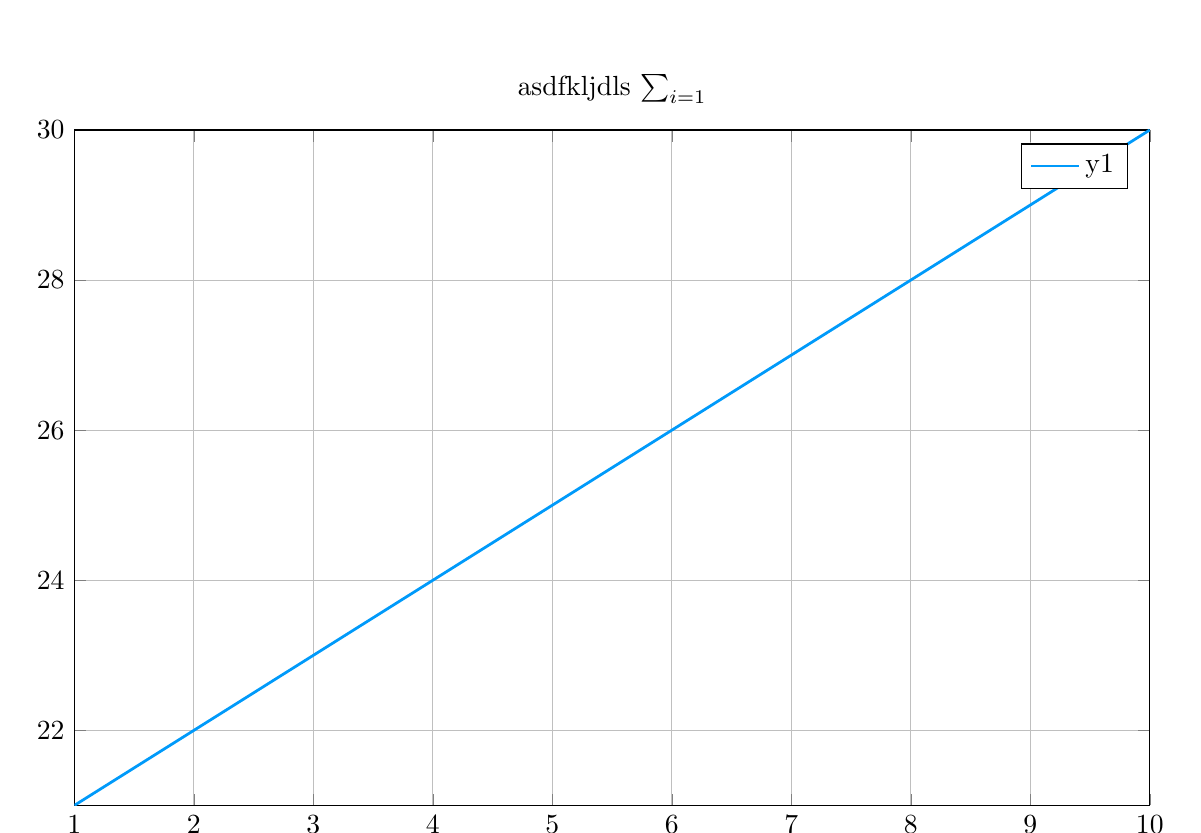
\begin{tikzpicture}[]
\begin{axis}[width = {152.4mm}, title = {asdfkljdls $\sum_{i=1}$}, ymax = {30.0}, height = {101.6mm}, xlabel = {}, {unbounded coords=jump,     xshift = 0.0mm,
    yshift = 0.0mm,
    axis background/.style={fill={rgb,1:red,1.00000000;green,1.00000000;blue,1.00000000}}
, grid = major}, ylabel = {}, ymin = {21.0}, xmax = {10.0}, xmin = {1.0}]\addplot+ [color = {rgb,1:red,0.00000000;green,0.60560316;blue,0.97868012},
draw opacity=1.0,
line width=1,
solid,mark = none,
mark size = 2.0,
mark options = {
    color = {rgb,1:red,0.00000000;green,0.00000000;blue,0.00000000}, draw opacity = 1.0,
    fill = {rgb,1:red,0.00000000;green,0.60560316;blue,0.97868012}, fill opacity = 1.0,
    line width = 1,
    rotate = 0,
    solid
}]coordinates {
(1, 21)
(2, 22)
(3, 23)
(4, 24)
(5, 25)
(6, 26)
(7, 27)
(8, 28)
(9, 29)
(10, 30)
};
\addlegendentry{y1}
\end{axis}

\end{tikzpicture}


\clearpage
\bibliographystyle{plain}
\bibliography{QR}

% \section{Appendices}
\label{appendice}

\subsection{Proof of quantiles as an optimization problem}
\label{sec:quantile-proof}
Let $Z^{\alpha}=\mbox{arg min}_{Q}E[\alpha\max\{0,X-Q\}+(1-\alpha)\max\{0,Q-X\}].$
We can rewrite the function as

\[
\begin{aligned}Y & =\alpha\int_{Q}^{\infty}(X-Q)dF_{x}+(1-\alpha)\int_{-\infty}^{Q}(Q-X)dF_{X}\\
& =\alpha\int_{Q}^{\infty}XdF_{x}-\alpha Q\int_{Q}^{\infty}QdF_{x}+Q\int_{-\infty}^{Q}dF_{x}-\int_{-\infty}^{Q}XdF_{x}-\alpha Q\int_{-\infty}^{Q}dF_{x}+\alpha\int_{-\infty}^{Q}XdF_{x}\\
& =\alpha\int_{Q}^{\infty}XdF_{x}-\alpha Q+QF_{X}(Q)-\int_{-\infty}^{Q}XdF_{x}-\alpha QF_{X}(Q)+\alpha\int_{-\infty}^{Q}XdF_{x}\\
& =\alpha\int_{Q}^{\infty}XdF_{x}-\alpha Q+QF_{X}(Q)-\int_{-\infty}^{Q}XdF_{x}+\alpha\int_{-\infty}^{Q}XdF_{x}
\end{aligned}
\]
By the first order condition for optimality, we need that $\frac{dZ(Q^{*})}{dQ}=0$.
So, we have:

\[
-\alpha Q^{*}f(Q^{*})-\alpha+F_{X}(Q^{*})+Q^{*}f(Q^{*})-Q^{*}f(Q^{*})+\alpha Q^{*}f(Q^{*})=0
\]
\[
F_{X}(Q^{*})=\alpha.
\]
Thus, we have that $Z^\alpha$ is the $\alpha-quantile$ of random variable $X$.

\subsection{MIP coefficients tables}
\label{sec:mipcoefficients}
The following tables inform the size of Coefficients when using the regularization method based on MIP described on session \ref{sec:best-subset-mip}. When using this method, we choose a parameter $K$ which defines the total number of nonzero coefficients (without accounting the intercept $\beta_0$, which is always included). 
In each column we find the estimated values of coefficients for each different choice of $K$. As coefficients are quantile dependent, we provide tables for $\alpha \in (0.05, 0.1, 0.25, 0.5, 0.75, 0.9, 0.95)$.

%\caption{\textbf{$\alpha = 0.05.} 

% latex table generated in R 3.2.3 by xtable 1.7-4 package
% Sat Apr 30 15:33:56 2016
\begin{table}[ht]
\centering
\begin{tabular}{rrrrrrrrrrrrr}
  \hline
 & K=1 & K=2 & K=3 & K=4 & K=5 & K=6 & K=7 & K=8 & K=9 & K=10 & K=11 & K=12 \\ 
  \hline
$\beta_{0}$ & -15.33 & 9.38 & 1.48 & 1.34 & 8.72 & -1.68 & 4.94 & 0.65 & -0.27 & -0.16 & -3.96 & -2.55 \\ 
  $\beta_{1}$ & -0.00 & 0.79 & 0.66 & 0.58 & 0.46 & 0.40 & 0.48 & 0.46 & 0.46 & 0.47 & 0.42 & 0.44 \\ 
  $\beta_{2}$ & -0.00 & -0.00 & -0.00 & -0.00 & -0.00 & 0.33 & -0.00 & -0.00 & -0.00 & -0.00 & 0.14 & 0.09 \\ 
  $\beta_{3}$ & -0.00 & -0.00 & -0.00 & -0.00 & -0.00 & -0.00 & -0.00 & 0.20 & 0.20 & 0.19 & 0.20 & 0.17 \\ 
  $\beta_{4}$ & -0.00 & -0.47 & -0.28 & -0.27 & -0.29 & -0.35 & -0.31 & -0.40 & -0.35 & -0.35 & -0.34 & -0.31 \\ 
  $\beta_{5}$ & -0.00 & -0.00 & -0.00 & -0.00 & -0.00 & -0.00 & -0.00 & -0.00 & -0.00 & -0.05 & -0.07 & -0.09 \\ 
  $\beta_{6}$ & -0.00 & -0.00 & -0.00 & -0.00 & -0.00 & -0.00 & 0.11 & 0.08 & 0.11 & 0.17 & 0.12 & 0.19 \\ 
  $\beta_{7}$ & -0.00 & -0.00 & -0.00 & -0.00 & -0.00 & -0.00 & -0.00 & -0.00 & -0.16 & -0.15 & -0.08 & -0.15 \\ 
  $\beta_{8}$ & -0.00 & -0.00 & -0.00 & -0.00 & -0.15 & -0.00 & -0.31 & -0.26 & -0.17 & -0.17 & -0.16 & -0.18 \\ 
  $\beta_{9}$ & -0.00 & -0.00 & -0.00 & -0.00 & -0.00 & 0.14 & 0.16 & 0.20 & 0.26 & 0.23 & 0.28 & 0.33 \\ 
  $\beta_{10}$ & -0.00 & -0.00 & -0.00 & -0.00 & -0.00 & -0.00 & -0.00 & -0.00 & -0.00 & -0.00 & -0.00 & -0.04 \\ 
  $\beta_{11}$ & -0.00 & -0.00 & 0.26 & 0.17 & 0.21 & 0.08 & 0.16 & 0.19 & 0.17 & 0.18 & 0.17 & 0.20 \\ 
  $\beta_{12}$ & 1.17 & -0.00 & -0.00 & 0.18 & 0.15 & 0.19 & 0.22 & 0.20 & 0.20 & 0.18 & 0.18 & 0.17 \\ 
   \hline
\end{tabular}
\caption{Coefficients for quantile $\alpha = 0.05$}
\end{table}

% latex table generated in R 3.2.3 by xtable 1.8-2 package
% Wed Apr 20 16:50:47 2016
\begin{table}[ht]
\centering
\begin{tabular}{rrrrrrrrrrrrr}
  \hline
 & K=1 & K=2 & K=3 & K=4 & K=5 & K=6 & K=7 & K=8 & K=9 & K=10 & K=11 & K=12 \\ 
  \hline
beta\_0 & -10.68 & 10.07 & 3.56 & 1.24 & 0.76 & 3.01 & 3.33 & 3.02 & 1.05 & 2.26 & 1.55 & 1.57 \\ 
  beta\_1 & -0.00 & 0.81 & 0.63 & 0.61 & 0.55 & 0.49 & 0.49 & 0.50 & 0.48 & 0.44 & 0.44 & 0.44 \\ 
  beta\_2 & -0.00 & -0.00 & -0.00 & -0.00 & -0.00 & -0.00 & 0.04 & -0.00 & -0.00 & 0.04 & 0.07 & 0.07 \\ 
  beta\_3 & -0.00 & -0.00 & -0.00 & -0.00 & 0.15 & 0.20 & 0.16 & 0.15 & 0.13 & 0.11 & 0.12 & 0.12 \\ 
  beta\_4 & -0.00 & -0.43 & -0.33 & -0.28 & -0.37 & -0.33 & -0.34 & -0.30 & -0.24 & -0.24 & -0.26 & -0.25 \\ 
  beta\_5 & -0.00 & -0.00 & -0.00 & -0.00 & -0.00 & -0.08 & -0.07 & -0.12 & -0.14 & -0.15 & -0.17 & -0.17 \\ 
  beta\_6 & -0.00 & -0.00 & -0.00 & -0.00 & -0.00 & -0.00 & -0.00 & 0.11 & 0.10 & 0.10 & 0.14 & 0.14 \\ 
  beta\_7 & -0.00 & -0.00 & -0.00 & -0.00 & -0.00 & -0.00 & -0.00 & -0.07 & -0.11 & -0.13 & -0.11 & -0.11 \\ 
  beta\_8 & -0.00 & -0.00 & -0.00 & -0.00 & -0.00 & -0.00 & -0.00 & -0.00 & -0.00 & -0.00 & -0.04 & -0.04 \\ 
  beta\_9 & -0.00 & -0.00 & -0.00 & -0.00 & -0.00 & -0.00 & -0.00 & -0.00 & 0.09 & 0.10 & 0.13 & 0.13 \\ 
  beta\_10 & -0.00 & -0.00 & -0.00 & -0.00 & -0.00 & -0.00 & -0.00 & -0.00 & -0.00 & -0.00 & -0.00 & 0.00 \\ 
  beta\_11 & -0.00 & -0.00 & -0.00 & 0.14 & 0.17 & 0.17 & 0.16 & 0.15 & 0.11 & 0.09 & 0.08 & 0.08 \\ 
  beta\_12 & 1.09 & -0.00 & 0.35 & 0.27 & 0.25 & 0.22 & 0.22 & 0.26 & 0.33 & 0.34 & 0.33 & 0.33 \\ 
   \hline
\end{tabular}
\end{table}

% latex table generated in R 3.2.3 by xtable 1.7-4 package
% Mon Apr 18 18:43:05 2016
\begin{table}[ht]
\centering
\begin{tabular}{rrrrrrrrrrrrr}
  \hline
 & K=1 & K=2 & K=3 & K=4 & K=5 & K=6 & K=7 & K=8 & K=9 & K=10 & K=11 & K=12 \\ 
  \hline
beta\_0 & 2.72 & -3.38 & 8.64 & 4.88 & 0.62 & 2.98 & 2.70 & 2.62 & 2.27 & 1.87 & 2.43 & 2.53 \\ 
  beta\_1 & -0.00 & 0.59 & 0.52 & 0.51 & 0.57 & 0.54 & 0.56 & 0.56 & 0.58 & 0.58 & 0.57 & 0.57 \\ 
  beta\_2 & -0.00 & -0.00 & -0.00 & -0.00 & -0.00 & -0.00 & -0.00 & -0.00 & -0.03 & -0.06 & -0.05 & -0.05 \\ 
  beta\_3 & -0.00 & -0.00 & -0.00 & -0.00 & -0.00 & -0.00 & -0.00 & -0.00 & -0.00 & 0.04 & 0.03 & 0.04 \\ 
  beta\_4 & -0.00 & -0.00 & -0.25 & -0.18 & -0.14 & -0.11 & -0.11 & -0.12 & -0.11 & -0.11 & -0.11 & -0.12 \\ 
  beta\_5 & -0.00 & -0.00 & -0.00 & -0.00 & -0.00 & -0.00 & -0.00 & -0.00 & -0.00 & -0.00 & -0.00 & 0.01 \\ 
  beta\_6 & -0.00 & -0.00 & -0.00 & -0.00 & -0.00 & -0.06 & -0.09 & -0.08 & -0.08 & -0.08 & -0.09 & -0.09 \\ 
  beta\_7 & -0.00 & -0.00 & -0.00 & -0.00 & -0.00 & -0.00 & -0.00 & -0.00 & -0.00 & -0.00 & -0.02 & -0.02 \\ 
  beta\_8 & -0.00 & -0.00 & -0.00 & -0.00 & -0.00 & -0.00 & 0.06 & 0.06 & 0.05 & 0.06 & 0.08 & 0.07 \\ 
  beta\_9 & -0.00 & -0.00 & -0.00 & -0.00 & 0.08 & 0.09 & 0.06 & 0.09 & 0.07 & 0.07 & 0.08 & 0.08 \\ 
  beta\_10 & -0.00 & -0.00 & -0.00 & -0.00 & -0.00 & -0.00 & -0.00 & -0.05 & -0.04 & -0.05 & -0.05 & -0.05 \\ 
  beta\_11 & -0.00 & 0.54 & -0.00 & 0.15 & 0.14 & 0.11 & 0.10 & 0.11 & 0.14 & 0.14 & 0.15 & 0.14 \\ 
  beta\_12 & 0.92 & -0.00 & 0.42 & 0.34 & 0.32 & 0.33 & 0.32 & 0.34 & 0.33 & 0.34 & 0.32 & 0.33 \\ 
   \hline
\end{tabular}
\end{table}

% latex table generated in R 3.2.3 by xtable 1.7-4 package
% Mon Apr 18 18:43:05 2016
\begin{table}[ht]
\centering
\begin{tabular}{rrrrrrrrrrrrr}
  \hline
 & K=1 & K=2 & K=3 & K=4 & K=5 & K=6 & K=7 & K=8 & K=9 & K=10 & K=11 & K=12 \\ 
  \hline
beta\_0 & 12.14 & 10.06 & 6.60 & 11.05 & 13.22 & 12.04 & 13.34 & 13.28 & 12.58 & 13.69 & 13.47 & 13.71 \\ 
  beta\_1 & -0.00 & 0.24 & 0.39 & 0.39 & 0.40 & 0.38 & 0.38 & 0.38 & 0.38 & 0.40 & 0.40 & 0.40 \\ 
  beta\_2 & -0.00 & -0.00 & -0.00 & -0.00 & -0.00 & -0.00 & -0.00 & -0.00 & -0.00 & -0.00 & -0.00 & -0.02 \\ 
  beta\_3 & -0.00 & -0.00 & -0.00 & -0.00 & -0.00 & -0.00 & -0.00 & -0.00 & -0.01 & -0.04 & -0.03 & -0.02 \\ 
  beta\_4 & -0.00 & -0.00 & -0.00 & -0.00 & -0.00 & -0.00 & -0.00 & 0.03 & -0.00 & 0.05 & 0.05 & 0.04 \\ 
  beta\_5 & -0.00 & -0.00 & -0.00 & -0.00 & -0.00 & -0.00 & -0.00 & -0.00 & -0.00 & -0.00 & 0.00 & 0.01 \\ 
  beta\_6 & -0.00 & -0.00 & -0.00 & -0.14 & -0.00 & -0.00 & -0.03 & -0.05 & -0.01 & -0.07 & -0.07 & -0.07 \\ 
  beta\_7 & -0.00 & -0.00 & -0.00 & -0.00 & -0.19 & -0.10 & -0.10 & -0.11 & -0.09 & -0.11 & -0.11 & -0.10 \\ 
  beta\_8 & -0.00 & -0.00 & -0.00 & -0.00 & -0.00 & -0.08 & -0.07 & -0.08 & -0.08 & -0.07 & -0.07 & -0.08 \\ 
  beta\_9 & -0.00 & -0.00 & -0.00 & 0.14 & 0.16 & 0.15 & 0.16 & 0.18 & 0.16 & 0.19 & 0.19 & 0.19 \\ 
  beta\_10 & -0.00 & -0.00 & -0.00 & -0.00 & -0.00 & -0.00 & -0.00 & -0.00 & -0.04 & -0.06 & -0.06 & -0.06 \\ 
  beta\_11 & -0.00 & -0.00 & 0.20 & -0.00 & 0.11 & 0.15 & 0.12 & 0.16 & 0.16 & 0.18 & 0.18 & 0.19 \\ 
  beta\_12 & 0.80 & 0.63 & 0.39 & 0.42 & 0.26 & 0.29 & 0.28 & 0.23 & 0.29 & 0.24 & 0.24 & 0.25 \\ 
   \hline
\end{tabular}
\end{table}

% latex table generated in R 3.2.3 by xtable 1.7-4 package
% Sat Apr 30 15:33:56 2016
\begin{table}[ht]
\centering
\begin{tabular}{rrrrrrrrrrrrr}
  \hline
 & K=1 & K=2 & K=3 & K=4 & K=5 & K=6 & K=7 & K=8 & K=9 & K=10 & K=11 & K=12 \\ 
  \hline
$\beta_{0}$ & 16.73 & 11.74 & 11.51 & 13.77 & 13.45 & 13.48 & 14.36 & 14.84 & 12.36 & 14.04 & 13.09 & 14.00 \\ 
  $\beta_{1}$ & -0.00 & 0.26 & 0.32 & 0.35 & 0.38 & 0.38 & 0.40 & 0.43 & 0.40 & 0.40 & 0.39 & 0.39 \\ 
  $\beta_{2}$ & -0.00 & -0.00 & -0.00 & -0.00 & -0.00 & -0.00 & -0.00 & -0.00 & -0.00 & -0.00 & 0.02 & 0.02 \\ 
  $\beta_{3}$ & -0.00 & -0.00 & -0.00 & -0.00 & -0.00 & -0.00 & -0.00 & -0.00 & -0.00 & -0.00 & -0.00 & 0.01 \\ 
  $\beta_{4}$ & -0.00 & -0.00 & -0.00 & -0.00 & -0.00 & -0.00 & -0.00 & -0.00 & 0.04 & 0.06 & 0.06 & 0.05 \\ 
  $\beta_{5}$ & -0.00 & -0.00 & -0.00 & -0.00 & -0.00 & -0.00 & -0.00 & -0.00 & -0.00 & -0.04 & -0.03 & -0.04 \\ 
  $\beta_{6}$ & -0.00 & -0.00 & -0.00 & -0.00 & -0.00 & -0.00 & -0.05 & -0.10 & -0.07 & -0.09 & -0.08 & -0.09 \\ 
  $\beta_{7}$ & -0.00 & -0.00 & -0.00 & -0.15 & -0.14 & -0.12 & -0.09 & -0.05 & -0.06 & -0.06 & -0.06 & -0.06 \\ 
  $\beta_{8}$ & -0.00 & -0.00 & -0.00 & -0.00 & -0.00 & -0.04 & -0.05 & -0.07 & -0.05 & -0.08 & -0.07 & -0.07 \\ 
  $\beta_{9}$ & -0.00 & -0.00 & -0.00 & 0.16 & 0.11 & 0.14 & 0.16 & 0.19 & 0.19 & 0.22 & 0.22 & 0.21 \\ 
  $\beta_{10}$ & -0.00 & -0.00 & -0.00 & -0.00 & -0.00 & -0.00 & -0.00 & -0.15 & -0.14 & -0.11 & -0.12 & -0.11 \\ 
  $\beta_{11}$ & -0.00 & -0.00 & 0.17 & -0.00 & 0.14 & 0.13 & 0.12 & 0.25 & 0.23 & 0.18 & 0.21 & 0.22 \\ 
  $\beta_{12}$ & 0.71 & 0.59 & 0.37 & 0.41 & 0.28 & 0.28 & 0.25 & 0.21 & 0.27 & 0.25 & 0.24 & 0.22 \\ 
   \hline
\end{tabular}
\end{table}

% latex table generated in R 3.3.2 by xtable 1.8-2 package
% Thu Feb  9 18:57:39 2017
\begin{table}[ht]
\centering
\begin{tabular}{rrrrrrrrrrrrr}
  \hline
 & Jan & Feb & Mar & Apr & May & Jun & Jul & Aug & Sep & Oct & Nov & Dec \\ 
  \hline
1981 & 23.36 & 28.34 & 12.44 & 18.35 & 17.10 & 22.49 & 23.57 & 40.10 & 48.40 & 42.13 & 43.70 & 37.23 \\ 
  1982 & 20.54 & 17.48 & 7.42 & 10.87 & 16.57 & 20.79 & 27.95 & 42.55 & 49.12 & 42.48 & 44.78 & 40.20 \\ 
  1983 & 27.94 & 24.50 & 22.60 & 22.24 & 29.62 & 27.05 & 33.92 & 45.06 & 50.64 & 49.32 & 43.83 & 36.14 \\ 
  1984 & 20.37 & 15.35 & 3.94 & 3.57 & 7.85 & 14.65 & 20.56 & 41.01 & 44.58 & 44.31 & 42.94 & 31.65 \\ 
  1985 & 10.38 & 4.71 & 5.15 & 2.84 & 7.27 & 10.36 & 14.53 & 39.33 & 45.18 & 41.21 & 42.15 & 23.02 \\ 
  1986 & 18.86 & 8.25 & 3.00 & 5.23 & 17.29 & 17.85 & 23.08 & 41.36 & 48.30 & 42.83 & 44.36 & 36.41 \\ 
  1987 & 26.09 & 24.71 & 6.90 & 21.02 & 20.73 & 19.53 & 28.42 & 42.94 & 48.06 & 44.26 & 43.11 & 39.67 \\ 
  1988 & 15.75 & 11.66 & 4.51 & 4.36 & 8.29 & 11.50 & 19.10 & 38.40 & 46.47 & 44.80 & 41.79 & 22.40 \\ 
  1989 & 19.92 & 14.52 & 5.08 & 2.75 & 5.62 & 11.42 & 17.17 & 38.94 & 43.92 & 43.70 & 40.69 & 26.34 \\ 
  1990 & 29.74 & 11.70 & 15.69 & 14.02 & 14.85 & 22.28 & 24.02 & 44.55 & 48.18 & 44.66 & 41.51 & 32.41 \\ 
  1991 & 17.09 & 13.46 & 7.68 & 6.63 & 8.51 & 16.17 & 26.46 & 43.36 & 49.00 & 45.86 & 40.14 & 36.57 \\ 
  1992 & 21.41 & 19.78 & 14.25 & 21.45 & 24.24 & 24.64 & 30.34 & 45.43 & 51.33 & 47.66 & 44.50 & 37.97 \\ 
  1993 & 27.86 & 20.13 & 14.36 & 16.63 & 20.94 & 26.43 & 30.60 & 44.07 & 44.73 & 43.78 & 41.40 & 34.18 \\ 
  1994 & 12.45 & 11.06 & 4.70 & 5.85 & 10.49 & 11.04 & 23.03 & 38.50 & 48.92 & 47.30 & 44.97 & 36.55 \\ 
  1995 & 20.31 & 5.80 & 9.47 & 5.36 & 5.62 & 14.15 & 23.54 & 42.48 & 50.49 & 42.74 & 41.15 & 29.90 \\ 
  1996 & 19.89 & 11.85 & 3.43 & 5.08 & 8.26 & 16.29 & 24.89 & 40.52 & 48.44 & 44.92 & 40.15 & 36.37 \\ 
  1997 & 23.89 & 27.80 & 14.30 & 11.95 & 17.55 & 22.22 & 31.82 & 44.07 & 43.14 & 40.00 & 37.94 & 28.36 \\ 
  1998 & 15.04 & 21.70 & 10.61 & 17.28 & 21.57 & 22.31 & 27.26 & 42.45 & 49.04 & 46.76 & 37.22 & 35.74 \\ 
  1999 & 22.18 & 15.39 & 8.18 & 13.66 & 8.67 & 16.49 & 22.30 & 40.43 & 47.75 & 39.85 & 36.95 & 35.54 \\ 
  2000 & 16.75 & 7.95 & 11.33 & 10.47 & 16.73 & 15.07 & 18.90 & 38.91 & 44.26 & 46.34 & 41.98 & 31.62 \\ 
  2001 & 24.03 & 11.82 & 11.09 & 9.23 & 16.30 & 14.53 & 25.73 & 41.57 & 45.79 & 40.99 & 41.52 & 42.76 \\ 
  2002 & 16.81 & 22.08 & 13.40 & 11.07 & 15.71 & 17.52 & 26.55 & 41.64 & 45.80 & 45.94 & 40.64 & 30.58 \\ 
  2003 & 17.42 & 14.05 & 10.03 & 11.26 & 15.39 & 17.01 & 28.29 & 39.98 & 47.02 & 47.07 & 40.47 & 34.85 \\ 
  2004 & 15.04 & 13.34 & 17.84 & 16.97 & 20.10 & 19.48 & 25.03 & 40.11 & 48.25 & 47.21 & 44.13 & 35.79 \\ 
  2005 & 24.89 & 20.47 & 13.01 & 20.88 & 19.98 & 21.48 & 27.81 & 42.74 & 46.09 & 46.93 & 44.98 & 36.08 \\ 
  2006 & 32.48 & 15.44 & 12.93 & 6.59 & 12.19 & 19.08 & 27.79 & 40.72 & 46.01 & 44.38 & 42.85 & 33.99 \\ 
  2007 & 28.93 & 11.13 & 16.10 & 11.91 & 17.68 & 21.57 & 30.56 & 42.95 & 47.80 & 47.61 & 42.97 & 35.98 \\ 
  2008 & 20.42 & 15.46 & 3.51 & 9.37 & 8.71 & 13.02 & 23.61 & 36.93 & 45.82 & 46.49 & 43.91 & 35.19 \\ 
  2009 & 21.48 & 15.16 & 6.74 & 3.80 & 4.48 & 12.88 & 24.53 & 38.40 & 47.70 & 40.87 & 46.73 & 38.03 \\ 
  2010 & 24.75 & 30.70 & 16.99 & 16.95 & 15.72 & 16.86 & 27.43 & 43.18 & 48.71 & 35.79 & 41.30 & 30.15 \\ 
  2011 & 16.33 & 14.79 & 9.30 & 7.70 & 13.35 & 18.60 & 23.53 & 39.62 & 46.97 & 40.99 & 44.75 & 42.79 \\ 
   \hline
\end{tabular}
\end{table}



%\subsection{Simulation study tables}
%\label{sec:simulation-tables}
%
%On section \ref{sec:simulation-ar1} we explain a simulation study to try evaluating differences between estimating a quantile with a quantile regression model or using the conditional mean when knowing the true generating model. From this experiment, we present below table of results for three different aspects, for five different quantiles. Tables from \ref{tab:sim-rmse-005} to \ref{tab:sim-rmse-095}  shows the difference between the root mean square errors between both methods of predicting the one-step ahead quantile for a few different values of $\alpha$. Tables \ref{tab:sim-auto-005}-\ref{tab:sim-auto-095} are the ones that shows the nominal difference between the autoregressive coefficients $\hat{\phi}$ and $\hat{\beta}$. The nominal difference between the intercept terms $\hat{\phi}_0 + z_\alpha  \hat{\sigma}^2_\varepsilon)$ and $\hat{\beta}_0)$ is 
%
%% latex table generated in R 3.2.3 by xtable 1.8-2 package
% Tue May 24 17:06:45 2016
\begin{table}[ht]
\centering
\begin{tabular}{rrrrrr}
  \hline
$\phi \backslash RSN$ & 0.01 & 0.05 & 0.1 & 0.5 & 1 \\ 
  \hline
0.25 & 0.99454499 & 0.99987753 & 0.99726238 & 0.99996553 & 0.99997820 \\ 
  0.50 & 0.99928262 & 1.00002733 & 0.99902661 & 1.00017501 & 1.00072601 \\ 
  0.70 & 0.97952103 & 0.99154652 & 1.00049301 & 0.99991315 & 1.00014586 \\ 
  0.90 & 0.89928729 & 0.99117750 & 0.99730087 & 1.00106737 & 0.99970135 \\ 
   \hline
\end{tabular}
\caption{RMSE ratio ($RMSE^{QR} / RMSE^{AR} $) for estimating quantile
$\alpha = $ 0.05. $\phi$ stands for the autoregressive coefficient 
and RSN is the signal to noise ratio. Details for these experiments can 
be found on section \ref{sec:simulation-ar1}} 
\label{tab:sim-rmse-005}
\end{table}

%% latex table generated in R 3.2.3 by xtable 1.8-2 package
% Tue May 24 17:06:45 2016
\begin{table}[ht]
\centering
\begin{tabular}{rrrrrr}
  \hline
$\phi \backslash RSN$ & 0.01 & 0.05 & 0.1 & 0.5 & 1 \\ 
  \hline
0.25 & 0.99404378 & 1.00071379 & 0.99865043 & 1.00009650 & 1.00031150 \\ 
  0.50 & 0.99302385 & 1.00012893 & 1.00008177 & 1.00020172 & 0.99997679 \\ 
  0.70 & 0.96163465 & 0.99948879 & 1.00007350 & 1.00076714 & 1.00002219 \\ 
  0.90 & 0.82867689 & 0.99989835 & 1.00007245 & 0.99997754 & 1.00016876 \\ 
   \hline
\end{tabular}
\caption{RMSE ratio ($RMSE^{QR} / RMSE^{AR} $) for estimating quantile
$\alpha = $ 0.1. $\phi$ stands for the autoregressive coefficient 
and RSN is the signal to noise ratio. Details for these experiments can 
be found on section \ref{sec:simulation-ar1}} 
\label{tab:sim-rmse-01}
\end{table}

%% latex table generated in R 3.2.3 by xtable 1.8-2 package
% Tue May 24 17:06:46 2016
\begin{table}[ht]
\centering
\begin{tabular}{rrrrrr}
  \hline
$\phi \backslash RSN$ & 0.01 & 0.05 & 0.1 & 0.5 & 1 \\ 
  \hline
0.25 & 0.98066380 & 0.99981708 & 0.99972368 & 1.00003875 & 1.00027661 \\ 
  0.50 & 0.99671712 & 0.99884992 & 0.99718531 & 0.99996169 & 0.99939155 \\ 
  0.70 & 0.96160330 & 0.99971110 & 1.00006113 & 1.00001116 & 1.00024519 \\ 
  0.90 & 0.93616426 & 0.99985323 & 0.99934405 & 0.99991411 & 0.99994730 \\ 
   \hline
\end{tabular}
\caption{RMSE ratio ($RMSE^{QR} / RMSE^{AR} $) for estimating quantile
$\alpha = $ 0.5. $\phi$ stands for the autoregressive coefficient 
and RSN is the signal to noise ratio. Details for these experiments can 
be found on section \ref{sec:simulation-ar1}} 
\label{tab:sim-rmse-05}
\end{table}

%% latex table generated in R 3.2.3 by xtable 1.8-2 package
% Tue May 24 17:06:46 2016
\begin{table}[ht]
\centering
\begin{tabular}{rrrrrr}
  \hline
$\phi \backslash RSN$ & 0.01 & 0.05 & 0.1 & 0.5 & 1 \\ 
  \hline
0.25 & 0.99662610 & 0.99945043 & 0.99538478 & 0.99966478 & 1.00025526 \\ 
  0.50 & 1.00028533 & 0.99613341 & 0.99981279 & 0.99996292 & 1.00108295 \\ 
  0.70 & 0.91878126 & 0.99889801 & 0.99885007 & 1.00023457 & 1.00067966 \\ 
  0.90 & 0.80536841 & 0.99826964 & 0.99806239 & 1.00003275 & 0.99993464 \\ 
   \hline
\end{tabular}
\caption{RMSE ratio ($RMSE^{QR} / RMSE^{AR} $) for estimating quantile
$\alpha = $ 0.9. $\phi$ stands for the autoregressive coefficient 
and RSN is the signal to noise ratio. Details for these experiments can 
be found on section \ref{sec:simulation-ar1}} 
\label{tab:sim-rmse-09}
\end{table}

%% latex table generated in R 3.2.3 by xtable 1.8-2 package
% Tue May 24 17:06:46 2016
\begin{table}[ht]
\centering
\begin{tabular}{rrrrrr}
  \hline
$\phi \backslash RSN$ & 0.01 & 0.05 & 0.1 & 0.5 & 1 \\ 
  \hline
0.25 & 1.00009586 & 0.99962843 & 1.00162321 & 1.00002799 & 1.00023607 \\ 
  0.50 & 0.99977885 & 0.99742853 & 0.99415437 & 1.00058173 & 0.99971703 \\ 
  0.70 & 0.93295124 & 0.99948015 & 0.99936096 & 1.00048504 & 0.99969376 \\ 
  0.90 & 0.97068193 & 1.00001858 & 1.00007662 & 1.00020540 & 0.99928392 \\ 
   \hline
\end{tabular}
\caption{RMSE ratio ($RMSE^{QR} / RMSE^{AR} $) for estimating quantile
$\alpha = $ 0.95. $\phi$ stands for the autoregressive coefficient 
and RSN is the signal to noise ratio. Details for these experiments can 
be found on section \ref{sec:simulation-ar1}} 
\label{tab:sim-rmse-095}
\end{table}

%
%% latex table generated in R 3.2.3 by xtable 1.8-2 package
% Tue May 24 17:06:45 2016
\begin{table}[ht]
\centering
\begin{tabular}{rrrrrr}
  \hline
$\phi \backslash RSN$ & 0.01 & 0.05 & 0.1 & 0.5 & 1 \\ 
  \hline
0.25 & -0.02501316 & 0.01504215 & -0.00565925 & -0.01735387 & -0.00060544 \\ 
  0.50 & -0.01319163 & 0.00222293 & 0.00477565 & 0.01005289 & -0.01981673 \\ 
  0.70 & 0.02775786 & -0.01203545 & 0.01320180 & -0.00721887 & -0.00665778 \\ 
  0.90 & 0.01743705 & 0.00303553 & 0.01319473 & -0.01785909 & 0.00046374 \\ 
   \hline
\end{tabular}
\caption{Diffeference between the autoregressive coefficients ($\hat{\phi} - \hat{\beta}$) for estimating quantile
$\alpha = $ 0.05. $\phi$ stands for the autoregressive coefficient 
and RSN is the signal to noise ratio. Details for these experiments can 
be found on section \ref{sec:simulation-ar1}} 
\label{tab:sim-auto-005}
\end{table}

%% latex table generated in R 3.2.3 by xtable 1.8-2 package
% Tue May 24 17:06:46 2016
\begin{table}[ht]
\centering
\begin{tabular}{rrrrrr}
  \hline
$\phi \backslash RSN$ & 0.01 & 0.05 & 0.1 & 0.5 & 1 \\ 
  \hline
0.25 & -0.00866846 & 0.02731984 & 0.01494079 & -0.01572119 & 0.01000855 \\ 
  0.50 & 0.02547593 & 0.00642516 & 0.00247766 & -0.00871352 & 0.00277974 \\ 
  0.70 & 0.00503748 & 0.00751987 & -0.00107390 & 0.00327506 & -0.00044987 \\ 
  0.90 & 0.00709175 & 0.00692367 & -0.00624776 & 0.00298916 & -0.00493012 \\ 
   \hline
\end{tabular}
\caption{Diffeference between the autoregressive coefficients ($\hat{\phi} - \hat{\beta}$) for estimating quantile
$\alpha = $ 0.1. $\phi$ stands for the autoregressive coefficient 
and RSN is the signal to noise ratio. Details for these experiments can 
be found on section \ref{sec:simulation-ar1}} 
\label{tab:sim-auto-01}
\end{table}

%% latex table generated in R 3.2.3 by xtable 1.8-2 package
% Tue May 24 17:06:46 2016
\begin{table}[ht]
\centering
\begin{tabular}{rrrrrr}
  \hline
$\phi \backslash RSN$ & 0.01 & 0.05 & 0.1 & 0.5 & 1 \\ 
  \hline
0.25 & 0.00504450 & -0.00552938 & 0.00198665 & 0.00331038 & 0.00493278 \\ 
  0.50 & 0.00816919 & -0.00518034 & -0.00514326 & 0.00056696 & 0.00347201 \\ 
  0.70 & 0.00817503 & 0.00319246 & -0.00703127 & -0.00478434 & 0.00539972 \\ 
  0.90 & 0.01257091 & 0.00502689 & -0.00469782 & -0.00543626 & 0.00172323 \\ 
   \hline
\end{tabular}
\caption{Diffeference between the autoregressive coefficients ($\hat{\phi} - \hat{\beta}$) for estimating quantile
$\alpha = $ 0.5. $\phi$ stands for the autoregressive coefficient 
and RSN is the signal to noise ratio. Details for these experiments can 
be found on section \ref{sec:simulation-ar1}} 
\label{tab:sim-auto-05}
\end{table}

%% latex table generated in R 3.2.3 by xtable 1.8-2 package
% Tue May 24 17:06:46 2016
\begin{table}[ht]
\centering
\begin{tabular}{rrrrrr}
  \hline
$\phi \backslash RSN$ & 0.01 & 0.05 & 0.1 & 0.5 & 1 \\ 
  \hline
0.25 & 0.00063949 & -0.00587333 & -0.00343132 & 0.00057888 & -0.01576153 \\ 
  0.50 & -0.01953741 & -0.00099696 & -0.01220643 & -0.00459181 & -0.02725897 \\ 
  0.70 & 0.00879188 & -0.00578564 & -0.01365016 & -0.01735324 & -0.01595786 \\ 
  0.90 & -0.00432531 & -0.00674863 & 0.00059043 & 0.00040195 & 0.00452383 \\ 
   \hline
\end{tabular}
\caption{Diffeference between the autoregressive coefficients ($\hat{\phi} - \hat{\beta}$) for estimating quantile
$\alpha = $ 0.9. $\phi$ stands for the autoregressive coefficient 
and RSN is the signal to noise ratio. Details for these experiments can 
be found on section \ref{sec:simulation-ar1}} 
\label{tab:sim-auto-09}
\end{table}

%% latex table generated in R 3.2.3 by xtable 1.8-2 package
% Tue May 24 17:06:46 2016
\begin{table}[ht]
\centering
\begin{tabular}{rrrrrr}
  \hline
$\phi \backslash RSN$ & 0.01 & 0.05 & 0.1 & 0.5 & 1 \\ 
  \hline
0.25 & -0.00217703 & 0.01773060 & -0.01892853 & 0.01070602 & -0.01105531 \\ 
  0.50 & -0.01530692 & -0.01035399 & -0.02514421 & 0.01278911 & -0.00835432 \\ 
  0.70 & 0.04323376 & -0.00354721 & 0.03589676 & -0.00176410 & -0.00545403 \\ 
  0.90 & 0.04279246 & 0.00727074 & -0.00552405 & 0.00634520 & -0.00118189 \\ 
   \hline
\end{tabular}
\caption{Diffeference between the autoregressive coefficients ($\hat{\phi} - \hat{\beta}$) for estimating quantile
$\alpha = $ 0.95. $\phi$ stands for the autoregressive coefficient 
and RSN is the signal to noise ratio. Details for these experiments can 
be found on section \ref{sec:simulation-ar1}} 
\label{tab:sim-auto-095}
\end{table}

%
%% latex table generated in R 3.2.3 by xtable 1.8-2 package
% Tue May 24 17:06:45 2016
\begin{table}[ht]
\centering
\begin{tabular}{rrrrrr}
  \hline
$\phi \backslash RSN$ & 0.01 & 0.05 & 0.1 & 0.5 & 1 \\ 
  \hline
0.25 & 0.04603811 & -0.01775659 & -0.03214647 & 0.02145871 & -0.00765273 \\ 
  0.50 & 0.03352012 & -0.00448700 & -0.02823629 & -0.04445694 & 0.03234653 \\ 
  0.70 & -0.04953532 & 0.10768253 & -0.03871770 & 0.02006049 & 0.01848257 \\ 
  0.90 & -0.01908312 & 0.05744539 & -0.17970986 & 0.12894696 & 0.02136838 \\ 
   \hline
\end{tabular}
\caption{Coefficient difference between the non-autoregressive part (($\hat{\phi}_0 + z_\alpha  \hat{\sigma}^2_\varepsilon) - \hat{\beta}_0)$ for estimating quantile
$\alpha = $ 0.05. $\phi$ stands for the autoregressive coefficient 
and RSN is the signal to noise ratio. Details for these experiments can 
be found on section \ref{sec:simulation-ar1}} 
\label{tab:sim-intercept-005}
\end{table}

%\clearpage
%% latex table generated in R 3.2.3 by xtable 1.8-2 package
% Tue May 24 17:06:46 2016
\begin{table}[ht]
\centering
\begin{tabular}{rrrrrr}
  \hline
$\phi \backslash RSN$ & 0.01 & 0.05 & 0.1 & 0.5 & 1 \\ 
  \hline
0.25 & 0.02260184 & -0.04514987 & -0.04187708 & 0.02309700 & -0.02037122 \\ 
  0.50 & -0.03481513 & -0.01041481 & -0.00038617 & -0.00296439 & -0.01172149 \\ 
  0.70 & 0.03459960 & -0.03797767 & 0.01480016 & 0.04972062 & 0.01002299 \\ 
  0.90 & 0.14704364 & -0.06159980 & 0.08091946 & -0.03306211 & 0.01302636 \\ 
   \hline
\end{tabular}
\caption{Coefficient difference between the non-autoregressive part (($\hat{\phi}_0 + z_\alpha  \hat{\sigma}^2_\varepsilon) - \hat{\beta}_0)$ for estimating quantile
$\alpha = $ 0.1. $\phi$ stands for the autoregressive coefficient 
and RSN is the signal to noise ratio. Details for these experiments can 
be found on section \ref{sec:simulation-ar1}} 
\label{tab:sim-intercept-01}
\end{table}

%% latex table generated in R 3.2.3 by xtable 1.8-2 package
% Tue May 24 17:06:46 2016
\begin{table}[ht]
\centering
\begin{tabular}{rrrrrr}
  \hline
$\phi \backslash RSN$ & 0.01 & 0.05 & 0.1 & 0.5 & 1 \\ 
  \hline
0.25 & 0.01297018 & -0.00048766 & -0.01041199 & -0.01243439 & 0.02395973 \\ 
  0.50 & -0.00774322 & 0.03340235 & 0.04581712 & -0.00941144 & 0.02834337 \\ 
  0.70 & 0.02631287 & -0.00313672 & 0.05261023 & -0.00929484 & -0.05534836 \\ 
  0.90 & -0.00600514 & -0.01798551 & 0.01424034 & 0.07490435 & -0.10554228 \\ 
   \hline
\end{tabular}
\caption{Coefficient difference between the non-autoregressive part (($\hat{\phi}_0 + z_\alpha  \hat{\sigma}^2_\varepsilon) - \hat{\beta}_0)$ for estimating quantile
$\alpha = $ 0.5. $\phi$ stands for the autoregressive coefficient 
and RSN is the signal to noise ratio. Details for these experiments can 
be found on section \ref{sec:simulation-ar1}} 
\label{tab:sim-intercept-05}
\end{table}
 % clearpage aqui
%% latex table generated in R 3.2.3 by xtable 1.8-2 package
% Tue May 24 17:06:46 2016
\begin{table}[ht]
\centering
\begin{tabular}{rrrrrr}
  \hline
$\phi \backslash RSN$ & 0.01 & 0.05 & 0.1 & 0.5 & 1 \\ 
  \hline
0.25 & -0.01239889 & 0.02293524 & -0.02274380 & -0.01803445 & 0.00913629 \\ 
  0.50 & 0.03837217 & 0.01562634 & 0.02285269 & 0.00939266 & 0.08607257 \\ 
  0.70 & 0.05059941 & 0.03251627 & 0.07964660 & 0.06332138 & 0.06101961 \\ 
  0.90 & 0.27272743 & 0.10535168 & 0.04777041 & 0.02227744 & -0.04024329 \\ 
   \hline
\end{tabular}
\caption{Coefficient difference between the non-autoregressive part (($\hat{\phi}_0 + z_\alpha  \hat{\sigma}^2_\varepsilon) - \hat{\beta}_0)$ for estimating quantile
$\alpha = $ 0.9. $\phi$ stands for the autoregressive coefficient 
and RSN is the signal to noise ratio. Details for these experiments can 
be found on section \ref{sec:simulation-ar1}} 
\label{tab:sim-intercept-09}
\end{table}

%% latex table generated in R 3.2.3 by xtable 1.8-2 package
% Tue May 24 17:06:46 2016
\begin{table}[ht]
\centering
\begin{tabular}{rrrrrr}
  \hline
$\phi \backslash RSN$ & 0.01 & 0.05 & 0.1 & 0.5 & 1 \\ 
  \hline
0.25 & 0.00335900 & -0.03337376 & 0.03659738 & -0.02854912 & 0.01837794 \\ 
  0.50 & 0.03376431 & -0.00203817 & -0.00638700 & -0.06833761 & -0.00379743 \\ 
  0.70 & -0.07861339 & 0.02610872 & -0.11362453 & 0.05524907 & -0.00006457 \\ 
  0.90 & -0.33397830 & -0.06626543 & 0.05843421 & -0.05809618 & -0.04813865 \\ 
   \hline
\end{tabular}
\caption{Coefficient difference between the non-autoregressive part (($\hat{\phi}_0 + z_\alpha  \hat{\sigma}^2_\varepsilon) - \hat{\beta}_0)$ for estimating quantile
$\alpha = $ 0.95. $\phi$ stands for the autoregressive coefficient 
and RSN is the signal to noise ratio. Details for these experiments can 
be found on section \ref{sec:simulation-ar1}} 
\label{tab:sim-intercept-095}
\end{table}


\end{document}

